\باب{حسابی ایمپلیفائر}

\موٹا{ٹرانزسٹر}\حاشیہب{transistor}  کی ایجاد سے اب تک الیکٹرانکس کے میدان میں ناقابل یقین اور حیرت انگیز ترقی ہوئی ہے۔شروع میں الگ الگ ٹرانزسٹر استعمال کر کے الیکٹرانک ادوار بنائے جاتے تھے۔بعد میں سلیکان کی پتری\حاشیہب{silicon chip}  پر ایک سے زیادہ ٹرانزسٹر بنانے کا رجحان پیدا ہوا۔اس طرح \موٹا{مخلوط ادوار}\فرہنگ{مخلوط ادوار}\حاشیہب{integrated chip (IC)}  وجود میں آئے۔ایک مربع سنٹی میٹر رقبہ کی سلیکان پتری\حاشیہد{ہائیڈروجن اور آکسیجن کے ملاپ سے پانی \عددی{\ce{H2O}} بنتا ہے۔اسی طرح سلیکان اور آکسیجن کے ملاپ سے \عددی{\ce{SiO2}} یعنی ریت یا مٹی بنتی ہے} پر اربوں ٹرانزسٹر بنانا ممکن ہوا اور دیکھتے ہی دیکھتے الیکٹرانک اشیاء  زندگی کے ہر شعبے پر چھا گئیں۔

اس کتاب میں الیکٹرانک پرزہ جات کی کارکردگی اور ان کے استعمال سے الیکٹرانک ادوار بنانے پر غور کیا جائے گا۔پہلے باب میں \موٹا{حسابی ایمپلیفائر}\فرہنگ{حسابی ایمپلیفائر}\حاشیہب{operational amplifier (OPAMP)}  پر غور کیا جائے گا۔حسابی ایمپلیفائر در حقیقت کئی ٹرانزسٹر پر مبنی ایک نہایت مقبول مخلوط دور ہے جس کا استعمال، برقی پرزہ جات مثلاً مزاحمت، کپیسٹر وغیرہ  کی طرح، نہایت آسان ہے۔حسابی ایمپلیفائر کی اندرونی ساخت پر اس کتاب میں آگے جا کر ایک مکمل باب ہے۔

\حصہ{حسابی ایمپلیفائر کے سرے یا پنیے}
	
حسابی ایمپلیفائر کی علامت شکل \حوالہ{شکل_حسابی_ایمپلیفائر_کی_علامت} الف  میں دکھائی گئی ہے۔حسابی ایمپلیفائر کے عموماً تین سرے ہوتے ہیں جن میں سے دو اس کے داخلی اور ایک خارجی سرا ہوتا ہے۔یوں شکل-الف میں ایک نمبر پنیا\حاشیہد{پنیوں کو نمبر کرنے کا طریقہ جلد بتلایا جائے گا} اس کا خارجی سرا ہے جبکہ دو اور تین نمبر پنیے اس کے داخلی سرے ہیں۔شکل  الف     میں حسابی ایمپلیفائر کی علامت میں دو مزید طاقت کے سرے بھی دکھائے گئے ہیں جو حسابی ایمپلیفائر کو برقی طاقت مہیا کرنے کی خاطر استعمال ہوتے ہیں۔حسابی ایمپلیفائر اُسی وقت کام کر سکتا ہے جب ان طاقت کے پنیوں پر درکار برقی طاقت مہیا کی جائے۔شکل \حوالہ{شکل_حسابی_ایمپلیفائر_کی_علامت} ب میں چار نمبر سرا مثبت برقی طاقت کا سرا ہے لہٰذا اس  پر مثبت برقی دباو مہیا کی گئی ہے  جبکہ گیارہ نمبر سرا منفی طاقت کا سرا ہے لہٰذا اس  پر منفی برقی دباو مہیا کی گئی ہے۔حسابی ایمپلیفائر ان مہیا کردہ برقی دباو سے برقی طاقت حاصل کرتا ہے۔روایتی طور پر مثبت برقی دباو کو \عددی{V_{CC}} اور منفی برقی دباو  کو \عددی{V_{EE}} پکارا جاتا ہے۔یوں شکل میں \عددی{V_{CC}=\SI{+12}{\volt}}اور \عددی{V_{EE}=\SI{-12}{\volt}}ہیں۔
\begin{figure}
\centering
\includegraphics[scale=0.90]{opampSymbol}
\caption{حسابی ایمپلیفائر کی علامت}
\label{شکل_حسابی_ایمپلیفائر_کی_علامت}
\end{figure}
حسابی ایمپلیفائر کو عموماً شکل \حوالہ{شکل_حسابی_ایمپلیفائر_کی_علامت} الف کی علامت سے ظاہر کرتے ہوئے طاقت پنیوں کو نہیں دکھایا جاتا۔

مثبت برقی دباو اور منفی برقی دباو عموماً \موٹا{پیدا کار برقی دباو} سے مہیا کیا جاتا ہے۔اس کتاب میں اس آلہ کو \موٹا{پیدا کار برقی دباو}،  \موٹا{برقی دباو کی سپلائی}\حاشیہب{voltage source} یا \موٹا{طاقت کی سپلائی}\فرہنگ{طاقت کی سپلائی}\حاشیہب{power supply}  پکارا جائے گا۔

صنعت کار ایک یا ایک سے زیادہ تعداد میں حسابی ایمپلیفائر پلاسٹک کی ڈبیا میں بند کرتے ہیں۔شکل \حوالہ{شکل_حسابی_ایمپلیفائر_کی_ڈبیا} میں ایک ہی ڈبیا میں چار حسابی ایمپلیفائر دکھائے گئے ہیں۔ڈبیا میں بند تمام حسابی ایمپلیفائر کے \عددیء{V_{CC}} آپس میں جوڑ کر چار نمبر پنیا پر جبکہ  تمام \عددیء{V_{EE}}  کو آپس میں جوڑ کر گیارہ نمبر پنیا پر پہنچایا گیا ہے۔ڈبیا پر باریک کٹ لگایا جاتا ہے۔اس کٹ سے گھڑی کی الٹ سمت گھومتے ہوئے پنیوں کو نمبر کیا جاتا ہے۔شکل \حوالہ{شکل_حسابی_ایمپلیفائر_کی_علامت} میں حسابی ایمپلیفائر کے پنیوں پر  لکھے گئے نمبر ڈبیا کے پنیوں کو ظاہر کرتے ہیں۔ 
\begin{figure}
\centering
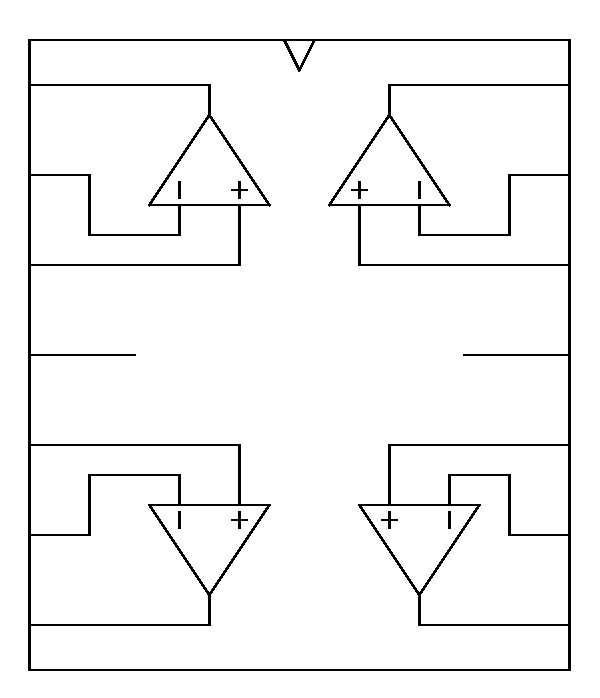
\includegraphics[scale=0.90]{opampLayout}
\caption{حسابی ایمپلیفائر کی ڈبیا}
\label{شکل_حسابی_ایمپلیفائر_کی_ڈبیا}
\end{figure}
\حصہ{حسابی ایمپلیفائر کی بنیادی کارکردگی}

حسابی ایمپلیفائر کی بنیادی کارکردگی کچھ یوں ہے۔اگر حسابی ایمپلیفائر کے دو داخلی سروں کے مابین \موٹا{تفرقی برقی اشارہ}\فرہنگ{تفرقی!برقی اشارہ} \عددی{v_d}\حاشیہب{differential voltage signal} مہیا کیا جائے تو یہ خارجی سرے پر\عددی{v_d} کو \عددی{A_d} گنا بڑھا کر خارج کرے گا، یعنی خارجی اشارہ \عددی{v_o}اور داخلی اشارہ \عددی{v_d}کا تعلق مندرجہ ذیل ہے
\begin{align} 
\label{مساوات_حسابی_بنیادی_کارکردگی}
v_o=A_d \times v_d
\end{align}
جہاں
\begin{align}
v_d=v_2-v_1
\end{align}
کے برابر ہے۔شکل \حوالہ{شکل_حسابی_ایمپلیفائر_کی_کارکردگی}  میں اس حقیقت کو دکھایا گیا ہے۔\عددی{A_d} کو ایمپلیفائر کا \موٹا{تفرقی برقی دباو کی افزائش}\فرہنگ{تفرقی!افزائش برقی دباو}\فرہنگ{differential voltage gain}\حاشیہب{differential voltage gain} یا \موٹا{برقی دباو کی تفرقی افزائش} کہتے ہیں۔یوں حسابی ایمپلیفائر کو \موٹا{تفرقی ایمپلیفائر}\فرہنگ{تفرقی!ایمپلیفائر}\حاشیہب{difference amplifier}\فرہنگ{amplifier!difference} بھی کہتے ہیں۔مساوات \حوالہ{مساوات_حسابی_بنیادی_کارکردگی}  میں اگر داخلی اشارہ کو دگنا کر دیا جائے تو خارجی اشارہ بھی دگنا ہو جائے گا۔یوں حسابی ایمپلیفائر کی کارکردگی \موٹا{خطی}\فرہنگ{خطی}\حاشیہب{linear relation} نوعیت کی ہے۔
	
یہاں اس بات کا ذکر کرنا ضروری ہے کہ حسابی ایمپلیفائر کے خارجی اشارہ \عددی{v_o}کی قیمت کسی صورت مثبت برقی دباو \عددی {V_{CC}} سے زیادہ یا منفی برقی دباو \عددی{V_{EE}} سے کم نہیں ہو سکتی۔ حقیقت میں \عددی{v_o} کی زیادہ سے زیادہ ممکنہ حد \عددی{V_{CC}}سے،\عددی{1} تا\عددی{3} وولٹ کم ہوتا ہے۔اسی طرح \عددی{v_o}کی کم سے کم ممکنہ حد  \عددی {V_{EE}}  سے، \عددی{1}  تا \عددی{3} وولٹ زیادہ ہوتا ہے۔یعنی
\begin{align}
\label{مساوات_حسابی_کے_خارجی_حدود}
(V_{EE} +\Delta_{-} )  <  v_o  < (V_{CC} -\Delta_{+})
\end{align}
اس مساوات میں \عددی{\Delta_{+}} اور \عددی{\Delta_{-}} ایک سے تین وولٹ کو ظاہر کرتے ہیں۔اس کتاب میں جب تک کہا نہ جائے ہم  \عددی{\Delta_{+}} اور  \عددی{\Delta_{-}} کی قیمت صفر تصور کریں گے۔یوں \عددی{v_o} مثبت برقی دباو \عددی{V_{CC}} سے لے کر منفی برقی دباو \عددی{V_{EE}}تک کی قیمت اختیار کر سکتا ہے۔حصہ \حوالہ{جزو_حسابی_ایمپلیفائر_کا_لبریز_ہونا} میں اس عمل پر تذکرہ کیا جائے گا۔



اگر حسابی ایمپلیفائر کو مہیا \موٹا{تفرقی اشارہ} \عددی{v_d}کی قیمت اتنی ہو کہ مساوات \حوالہ{مساوات_حسابی_بنیادی_کارکردگی}   سے حاصل \عددی{v_o} کی قیمت مساوات \حوالہ{مساوات_حسابی_کے_خارجی_حدود}  میں دیے حدود سے تجاوز کرے تو اس صورت میں حسابی ایمپلیفائر مساوات \حوالہ{مساوات_حسابی_بنیادی_کارکردگی}  پر پورا نہیں اترے گا جبکہ اس کی  \عددی{v_o}   مساوات \حوالہ{مساوات_حسابی_کے_خارجی_حدود}  میں دیے حدود کے اندر ہی رہے گی۔اس صورت میں مثبت جانب بڑھتے ہوئے\عددی{v_o}  کی قیمت \عددی{(V_{CC}-\Delta_{+})} تک پہنچ کر رک جائے گی یا پھر منفی جانب گھٹتے ہوئے \عددی{v_o} کی قیمت  \عددی{(V_{CC}-\Delta_{-})} تک پہنچ کر رک جائے گی۔اس صورت میں  \عددی{\abs{v_d}} کو مزید بڑھانے سے \عددی{v_o} کی قیمت پر کوئی اثر نہیں ہوتا۔اس صورت میں حسابی ایمپلیفائر کی کارکردگی غیر خطی ہو گی اور اس کو حسابی ایمپلیفائر کا \موٹا{لبریز}\فرہنگ{لبریز}
\فرہنگ{saturation!OPAMP}\حاشیہب{saturation}  ہونا کہتے ہیں۔
\begin{figure}
\centering
\includegraphics[scale=0.90]{opampWorking}
\caption{حسابی ایمپلیفائر کی کارکردگی}
\label{شکل_حسابی_ایمپلیفائر_کی_کارکردگی}
\end{figure}
%==============================
\ابتدا{مثال}
ایک حسابی ایمپلیفائر جس کی \موٹا{تفرقی افزائش برقی دباو} \عددی{A_d}  کی قیمت \عددی{\SI{100000}{\volt \per \volt}} ہے کو اس کے داخلی سروں پر مندرجہ ذیل برقی دباو مہیا کئے جاتے ہیں۔
\begin{enumerate}
\item
\عددی{v_1=\SI{0}{\volt}} اور \عددی{v_2 = \SI{10}{\micro \volt}}
\item
\عددی{v_1=\SI{10}{\micro \volt}} اور \عددی{v_2 = \SI{0}{\volt}}
\item
\عددی{v_1=\SI{2.00003}{\volt}} اور \عددی{v_2 = \SI{2.00005}{\volt}}
\item
\عددی{v_1=\SI{2.0003}{\volt}} اور \عددی{v_2 = \SI{2.0005}{\volt}}
\item
\عددی{v_1=\SI{2.05}{\volt}} اور \عددی{v_2 = \SI{2.03}{\volt}}

\item
\عددی{v_1=\SI{2.03}{\volt}} اور \عددی{v_2 =\SI{2.03}{\volt}}
\end{enumerate}
\عددی{V_{CC}=\SI{+12}{\volt}}اور \عددی{V_{EE}=\SI{-12}{\volt}} جبکہ \عددی{\Delta_+ = \Delta_- = 0} ہونے کی صورت میں حسابی ایمپلیفائر کی \عددی{v_o} دریافت کریں۔


حل:	جب تک \عددی{v_o} مساوات \حوالہ{مساوات_حسابی_کے_خارجی_حدود}  میں دیے حدود کے اندر رہے، حسابی ایمپلیفائر داخلی برقی دباو کو ایک لاکھ مرتبہ بڑھا کر خارج کرے گا۔یوں
\begin{enumerate}
\item $\begin{aligned}[t]
v_0 &=A_d \times v_d \\
&=A_d \times \left (v_2 - v_1 \right )\\
&=100000 \times \left(10\times 10^{-6}-0 \right )\\
&=\SI{1}{\volt}
\end{aligned}$
%
\item $\begin{aligned}[t]
v_0 &=A_d \times v_d \\
&=A_d \times \left (v_2 - v_1 \right )\\
&=100000 \times \left(0-10\times 10^{-6} \right )\\
&=\SI{-1}{\volt}
\end{aligned}$
%
\item $\begin{aligned}[t]
v_0 &=A_d \times v_d \\
&=A_d \times \left (v_2 - v_1 \right )\\
&=100000 \times \left(2.00005-2.00003 \right )\\
&=\SI{2}{\volt}
\end{aligned}$

\item $\begin{aligned}[t]
v_0 &=A_d \times v_d \\
&=A_d \times \left (v_2 - v_1 \right )\\
&=100000 \times \left(2.0005-2.0003 \right )\\
&=\SI{20}{\volt}
\end{aligned}$
چوتھے صورت میں \عددی{v_o} کی قیمت مساوات \حوالہ{مساوات_حسابی_کے_خارجی_حدود} میں دیے حدود سے تجاوز کر گئی جو کہ ناممکن صورتِ حال ہے۔لہٰذا اس جواب کو رد کیا جاتا ہے۔اس صورت میں حسابی ایمپلیفائر کی کوشش ہو گی کہ \عددی{v_o} کی قیمت بیس وولٹ ہو لیکن حسابی ایمپلیفائر ایسا کرنے سے عاجز ہے  کیونکہ اس کے خارجی اشارے  کی قیمت \عددی{V_{CC}} کی قیمت سے زیادہ نہیں ہو سکتی۔لہٰذا  \عددی{ \Delta_+ = \Delta_- = 0} لیتے ہوئے اس صورت میں  \عددی{v_o}زیادہ سے زیادہ ممکنہ برقی دباو کے برابر ہو گا یعنی \عددی{v_o = +12 V}ہو گا۔حقیقت میں  \عددی{v_o}کی زیادہ سے زیادہ ممکنہ قیمت\عددی{V_{CC}}  سے ایک یا دو وولٹ کم ہوتی ہے۔حسابی ایمپلیفائر بنانے والے یہ معلومات فراہم کرتے ہیں۔
\item $\begin{aligned}[t]
v_0 &=A_d \times v_d \\
&=A_d \times \left (v_2 - v_1 \right )\\
&=100000 \times \left(2.03-2.05 \right )\\
&=\SI{-2000}{\volt}
\end{aligned}$
یہاں \عددی{v_o} کی قیمت مساوات \حوالہ{مساوات_حسابی_کے_خارجی_حدود}  میں دیے حدود سے تجاوز کر گئی جو کہ ناممکن صورتِ حال ہے۔اس صورت میں  \عددی{v_o}کی قیمت  \عددی{V_{EE}} سے قدر زیادہ قیمت اختیار کرے گی۔ \عددی{\Delta_+ = \Delta_- = 0}لیتے ہوئے اس صورت\عددی{v_o=\SI{-12}{\volt}} ہو گی۔
\item $\begin{aligned}[t]
v_0 &=A_d \times v_d \\
&=A_d \times \left (v_2 - v_1 \right )\\
&=100000 \times \left(2.03-2.03 \right )\\
&=\SI{0}{\volt}
\end{aligned}$
\end{enumerate}
یہاں آپ نے دیکھا کہ دونوں داخلی سروں پر برابر برقی دباو مہیا کرنے سے حسابی ایمپلیفائر صفر وولٹ خارج کرتا ہے۔دونوں داخلی سروں پر برابر مہیا کردہ برقی دباو کو \موٹا{مشترکہ برقی دباو}\فرہنگ{مشترکہ برقی دباو}\فرہنگ{common mode voltage}\حاشیہب{common mode voltage}  کہتے ہیں۔حسابی ایمپلیفائر مشترکہ برقی دباو کو رد کرتا ہے۔


یہاں یہ بتلاتا چلوں کہ کسی بھی داخلی برقی دباو کو \موٹا{مشترکہ برقی دباو} \عددی{v_{CM}} اور \موٹا{تفرقی برقی دباو}\فرہنگ{تفرقی!برقی دباو}\فرہنگ{differential mode voltage}\حاشیہب{differential mode voltage} \عددی{v_d} میں تقسیم کیا جا سکتا ہے۔پانچویں جزو میں \عددی{v_1 = \SI{2.05}{\volt}} اور \عددی{v_2 = \SI{2.03}{\volt}} کو یوں بیان کیا جا سکتا ہے کہ حسابی ایمپلیفائر کو 
\( \tfrac{2.05+2.03}{2}=\SI{2.04}{\volt} \)
بطور مشترکہ برقی دباو فراہم کئے گئے جبکہ اسے
\( 2.03-2.05=\SI{-0.02}{\volt}\)
بطور تفرقی برقی دباو مہیا کئے گئے۔

\انتہا{مثال}
%=====================

	اس مثال میں آپ نے دیکھا کہ چند مائیکرو وولٹ\حاشیہب{\si{\micro \volt}} برقی دباو کو حسابی ایمپلیفائر بڑھا کر وولٹ کی حد میں لے آتا ہے۔یہاں آپ کی دلچسپی کی خاطر بتلاتا چلوں کہ انسانی اعصابی نظام  ستر ملی وولٹ \عددی{\SI{70}{\milli \volt}} کے لگ بھگ برقی دباو پر کام کرتا ہے۔یوں حسابی ایمپلیفائر استعمال کرتے ہوئے  آپ اعصابی نظام کے کارکردگی پر تحقیق کر سکتے ہیں۔ 

	اس مثال کے پہلے دو حصوں میں آپ نے دیکھا کہ اگر داخلی برقی دباو کو حسابی ایمپلیفائر کے \موٹا{مثبت داخلی سرے}\فرہنگ{مثبت داخلی سرا}\حاشیہب{non-inverting input}  پر مہیا کیا جائے تو اس سے حاصل خارجی برقی دباو کی علامت تبدیل نہیں ہوتی۔یعنی اگر مثبت برقی دباو مہیا کی جائے تو مثبت برقی دباو ہی خارج کی جاتی ہے۔اس کے برعکس اگر برقی دباو کو حسابی ایمپلیفائر کے \موٹا{منفی داخلی سرے}\فرہنگ{منفی داخلی سرا}\حاشیہب{inverting input}  پر مہیا کیا جائے تو اس سے حاصل خارجی برقی دباو کی علامت تبدیل ہو جاتی ہے۔یعنی اگر مثبت برقی دباو مہیا کی جائے تو منفی برقی دباو خارج کی جاتی ہے۔

\حصہ{ حسابی ایمپلیفائر کا مساوی دور}
حسابی ایمپلیفائر کا مساوی دور شکل \حوالہ{شکل_حسابی_ایمپلیفائر_کا_مساوی_دور} میں دکھایا\حاشیہد{اس شکل میں تفرقی برقی دباو کا مثبت سرا نچلی جانب ہے۔} گیا ہے۔
\begin{figure}
\centering
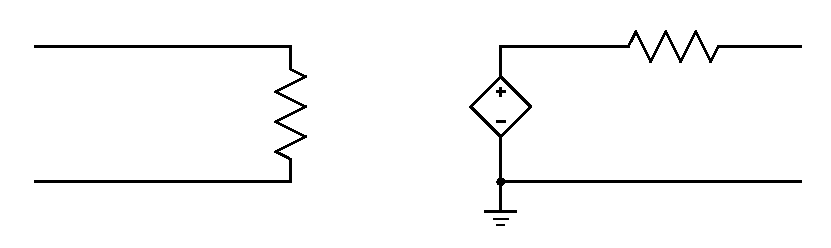
\includegraphics[scale=0.90]{opampEquivalentCircuit}
\caption{حسابی ایمپلیفائر کا مساوی دور}
\label{شکل_حسابی_ایمپلیفائر_کا_مساوی_دور}
\end{figure}
جیسا کہ شکل سے واضح ہے داخلی جانب سے حسابی ایمپلیفائر بالکل ایک مزاحمت \عددی{R_i} کی طرح معلوم ہوتا ہے جبکہ خارجی جانب  یہ  قابو برقی دباو کی سپلائی\حاشیہب{controlled voltage source}  جس کے ساتھ سلسلہ وار مزاحمت \عددی{R_o} جڑی ہو معلوم ہوتا ہے۔قابو برقی دباو کی سپلائی، داخلی جانب مہیا اشارہ \عددی{v_d}سے قابو ہوتا ہے۔

	حسابی ایمپلیفائر کے صنعت کاروں کی کوشش ہوتی ہے کہ حسابی ایمپلیفائر کے \موٹا{داخلی مزاحمت}\فرہنگ{داخلی مزاحمت} \عددی{R_i} کی قیمت زیادہ سے زیادہ جبکہ  \موٹا{خارجی مزاحمت}\فرہنگ{خارجی مزاحمت} \عددی{R_o} کی قیمت کم سے کم ہو۔اسی طرح کوشش کی جاتی ہے کہ \موٹا{تفرقی افزائش برقی دباو}\فرہنگ{تفرقی!افزائش برقی دباو}  \عددی{A_d} کی قیمت زیادہ سے زیادہ ہو۔جدول \حوالہ{جدول_حسابی_ایمپلیفائر_عمومی_مقداریں} میں آپ کے اندازے کی خاطر ایک عام دستیاب حسابی ایمپلیفائر\حاشیہد{عام دستیاب ایمپلیفائر کی قیمت بازار میں فروخت ہونے والی  تندور کی دو روٹیوں کے لگ بھگ ہے} کے  ماڈل کے اجزاء دئے گئے ہیں۔
\begin{table}[ht]
\caption{عام دستیاب حسابی ایمپلیفائر کی مقررہ مقداریں}
\label{جدول_حسابی_ایمپلیفائر_عمومی_مقداریں}
\centering
\begin{tabular}{l l}
\toprule
$R_i$ &  $\SI{e{12}}{\ohm}$ \\
$R_o$ & $\SI{100}{\ohm}$\\
$A_d$  & $\SI[per=frac,fraction=nice]{100000}{\volt \per \volt}$ \\
\bottomrule
\end{tabular}
\end{table}
ان مقداروں کو مثال بناتے ہوئے شکل \حوالہ{شکل_حسابی_ایمپلیفائر_کا_مساوی_دور} پر غور کرتے ہیں۔

\جزوحصہ{داخلی سروں پر برابر برقی دباو رہتا ہے}

حسابی ایمپلیفائر کو عام طور خطی کارکردگی کے احاطے میں استعمال کیا جاتا ہے یعنی اسے  استعمال کرتے ہوئے  \عددی{v_d} کی قیمت اتنی رکھی جاتی ہے کہ \عددی{v_o} مساوات \حوالہ{مساوات_حسابی_کے_خارجی_حدود} میں دیے حدود کے اندر رہے۔\عددی{V_{CC}=\SI{+12}{\volt}} اور \عددی{V_{EE}=\SI{-12}{\volt}} لیتے ہوئے \عددی{v_o} کی زیادہ سے زیادہ ممکنہ قیمت تقریباً \عددی{\SI{+12}{\volt}}اور کم سے کم ممکنہ قیمت تقریباً \عددی{\SI{-12}{\volt}} ہے۔جب \عددی{v_o = \SI{+12}{\volt}}ہو،  اس وقت مساوات \حوالہ{مساوات_حسابی_بنیادی_کارکردگی}  کے تحت \عددی{v_d =\SI{120}{\micro \volt}} ہو گا اور جب  \عددی{v_o = \SI{-12}{\volt}} ہو اس وقت\عددی{v_d =\SI{-120}{\micro \volt}} ہو گا۔یوں حسابی ایمپلیفائر کو خطی خطے میں استعمال کرتے ہوئے \عددی{\abs{v_d} < \SI{120}{\micro \volt}} رہے گا۔شکل \حوالہ{شکل_حسابی_ایمپلیفائر_کی_کارکردگی}  کو دیکھتے ہوئے اس بات کو یوں بیان کر سکتے ہیں کہ
\begin{align}
\abs{v_d} =\abs{v_2-v_1} < \SI{120}{\micro \volt}
\end{align}
رکھتے ہوئے حسابی ایمپلیفائر خطی خطے میں رہتا ہے۔\عددی{\SI{120}{\micro \volt}} اتنی کم برقی دباو ہے کہ اسے نظر انداز کیا جا سکتا ہے۔ایسا کرنے سے حسابی ایمپلیفائر پر مبنی ادوار کو حل کرنا نہایت آسان ہو جاتا ہے۔یوں  اس مساوات کو اس طرح لکھا جا سکتا ہے
\begin{gather}
\begin{aligned} \label{مساوات_حسابی_داخلی_سروں_پر_برابر_دباو}
\abs{v_2  -  v_1} &\approx 0   \\
v_2 & \approx v_1
\end{aligned}
\end{gather}
	یہ نہایت اہم مساوات ہے  جسے  بار بار استعمال کیا جائے گا۔اس مساوات کے تحت جب تک حسابی ایمپلیفائر کو خطی احاطے میں استعمال کیا جائے اس وقت تک اس کے دونوں داخلی سروں پر تقریباً برابر برقی دباو ہو گا۔

	اوپر مثال کو دوبارہ دیکھتے ہوئے پہلی دو صورتوں میں \عددی{v_2 \approx v_1 \approx 0}ہے جبکہ تیسری صورت میں \عددی{v_2 \approx v_1 \approx \SI{2}{\volt}} ہے۔ان میں حسابی ایمپلیفائر خطی احاطے میں کام کر رہا ہے۔چوتھی اور پانچویں صورتوں میں یہ غیر خطی احاطے میں کام کر رہا ہے۔پانچویں صورت میں یہ بات زیادہ واضح سامنے آتی ہے کہ \عددی{v_2} اور\عددی{v_1} برابر نہیں۔یہاں ان میں  \عددی{\SI{20}{\milli \volt}} کا فرق ہے جسے نظر انداز نہیں کیا جا سکتا۔

\جزوحصہ{داخلی سروں پر برقی رو صفر ہوتی ہے}
	آپ نے دیکھا کہ حسابی ایمپلیفائر کو خطی احاطے میں استعمال کرتے ہوئے  \عددی{\abs{v_d}< \SI{120}{\micro \volt}} رہتا ہے۔اگر \عددی{R_i=\SI{e12}{\ohm}}ہو تو شکل \حوالہ{شکل_حسابی_ایمپلیفائر_کا_مساوی_دور}  کو دیکھتے ہوئے مزاحمت \عددی{R_i}میں برقی رو \عددی{i} کی قیمت
\begin{align}
i=\frac{v_d}{R_i} =\frac{\abs{120 \times 10^{-6}}}{10^{12}}=\SI{1.2e-16}{\ampere}
\end{align}
ہو گی جو کہ قابل نظر انداز قیمت ہے۔یوں ہم کہہ سکتے ہیں کہ حسابی ایمپلیفائر کے داخلی سروں پر برقی رو کی قیمت صفر ایمپیئر ہو گی یا یہ کہ ان سروں کو مکمل طور منقطع تصور کیا جا سکتا ہے۔یوں
\begin{align} \label{مساوات_حسابی_صفر_داخلی_رو}
{i \approx \SI{0}{\ampere}}
\end{align}
تصور کیا جاتا ہے۔

\جزوحصہ{داخلی مزاحمت کو لامحدود تصور کیا جاتا ہے}

	جیسا کہ جدول  میں ذکر ہوا حسابی ایمپلیفائر کے داخلی مزاحمت \عددی{R_i}کی قیمت نہایت بڑی ہوتی ہے۔اتنی مزاحمت کو یقیناً لامحدود تصور کیا جا سکتا ہے یعنی
\begin{align} \label{مساوات_حسابی_لامحدود_داخلی_مزاحمت}
R_i \to \infty
\end{align}
اس کا مطلب ہے کہ داخلی سروں کو آپس میں مکمل طور منقطع سمجھا جا سکتا ہے۔


\جزوحصہ{تفرقی افزائش کو لامحدود تصور کیا جاتا ہے}

جدول \حوالہ{جدول_حسابی_ایمپلیفائر_عمومی_مقداریں} میں تفرقی افزائش برقی دباو کی مثال \عددی{A_d =\SI[per=frac,fraction=nice]{100000}{\volt \per \volt}} دی گئی ہے جسے لامحدود تصور کیا جا سکتا ہے یعنی
\begin{align}
A_D \to \infty
\end{align}
اس مساوات کو دیکھتے یہ خیال آتا ہے کہ لامحدود افزائش کی صورت میں اسے استعمال کیسے کیا جائے گا۔درحقیقت حسابی ایمپلیفائر کو عموماً واپسی اشارہ\حاشیہب{feedback signal}  مہیا کرتے ہوئے استعمال کیا جاتا۔اس بات کی وضاحت حصہ \حوالہ{حصہ_حسابی_ایمپلیفائر_کے_ادوار} میں ہو جائے گی۔


\جزوحصہ{خارجی مزاحمت کو صفر اُوہم تصور کیا جا سکتا ہے}
	
آپ دیکھیں گے کہ عام استعمال میں حسابی ایمپلیفائر کے خارجی جانب جڑے بیرونی مزاحمتوں کی قیمتیں کلو اُوہم  \عددیء{\SI{}{\kilo \ohm}} کے حدود میں ہو گی جو کہ  \عددی{R_o} کی قیمت سے کئی گنا زیادہ ہے۔یوں حسابی ایمپلیفائر پر مبنی ادوار حل کرتے وقت اگر\عددی{R_o} کو بالکل نظر انداز کر دیا جائے تو حاصل جواب پر خاص فرق نہیں پڑے گا۔عام استعمال میں ایسا ہی تصور کیا جاتا ہے یعنی
\begin{align} \label{مساوات_حسابی_صفر_خارجی_مزاحمت}
R_o \approx \SI{0}{\ohm}
\end{align}


\حصہ{کامل حسابی ایمپلیفائر}

خطی خطے  میں استعمال ہوتے ہوئے حسابی ایمپلیفائر  کی کارکردگی پر غور کرتے ہوئے کچھ حقائق سامنے آئے جنہیں مساوات \حوالہ{مساوات_حسابی_داخلی_سروں_پر_برابر_دباو}، \حوالہ{مساوات_حسابی_صفر_داخلی_رو} ،  \حوالہ{مساوات_حسابی_لامحدود_داخلی_مزاحمت} اور \حوالہ{مساوات_حسابی_صفر_خارجی_مزاحمت} میں بیان کیا گیا۔ان مساوات کو یہاں یکجا کر کے پیش کرتے ہیں۔
\begin{gather} 
\begin{aligned}\label{مساوات_حسابی_بنیادی_پہلو}
v_2 &=v_1 \hspace{5mm} \textrm{خطی خطہ}\\
i&=0\\
R_i &=\infty\\
R_o &=0
\end{aligned}
\end{gather}
ایسا کرتے وقت \عددی{\approx} اور\عددی{\to} کے علامات کی جگہ \عددی{=}کی علامت استعمال کی گئی ہے۔ان مساوات کے پہلے جزو میں خطی خطہ لکھ کر اس بات کی یاد دہانی کرائی جاتی ہے کہ داخلی سرے صرف اس صورت برابر برقی دباو پر رہتے ہیں جب تک ایمپلیفائر خطی خطے میں رہے۔اس بات کی وضاحت مثال \حوالہ{مثال_حسابی_خطی_غیر_خطی_خطے} میں ہو گی۔ان مساوات کو مد نظر رکھتے ہوئے ہم شکل \حوالہ{شکل_حسابی_ایمپلیفائر_کا_مساوی_دور}  کو دوبارہ بناتے ہیں۔ایسا کرنے سے شکل \حوالہ{شکل_کامل_حسابی_ایمپلیفائر_کا_مساوی_دور} حاصل ہوتا ہے جو کہ \موٹا{کامل} حسابی ایمپلیفائر\فرہنگ{کامل حسابی ایمپلیفائر}\حاشیہب{ideal} کا مساوی دور ہے۔
\begin{figure} \label{شکل_حسابی_کامل_ماڈل}
\centering
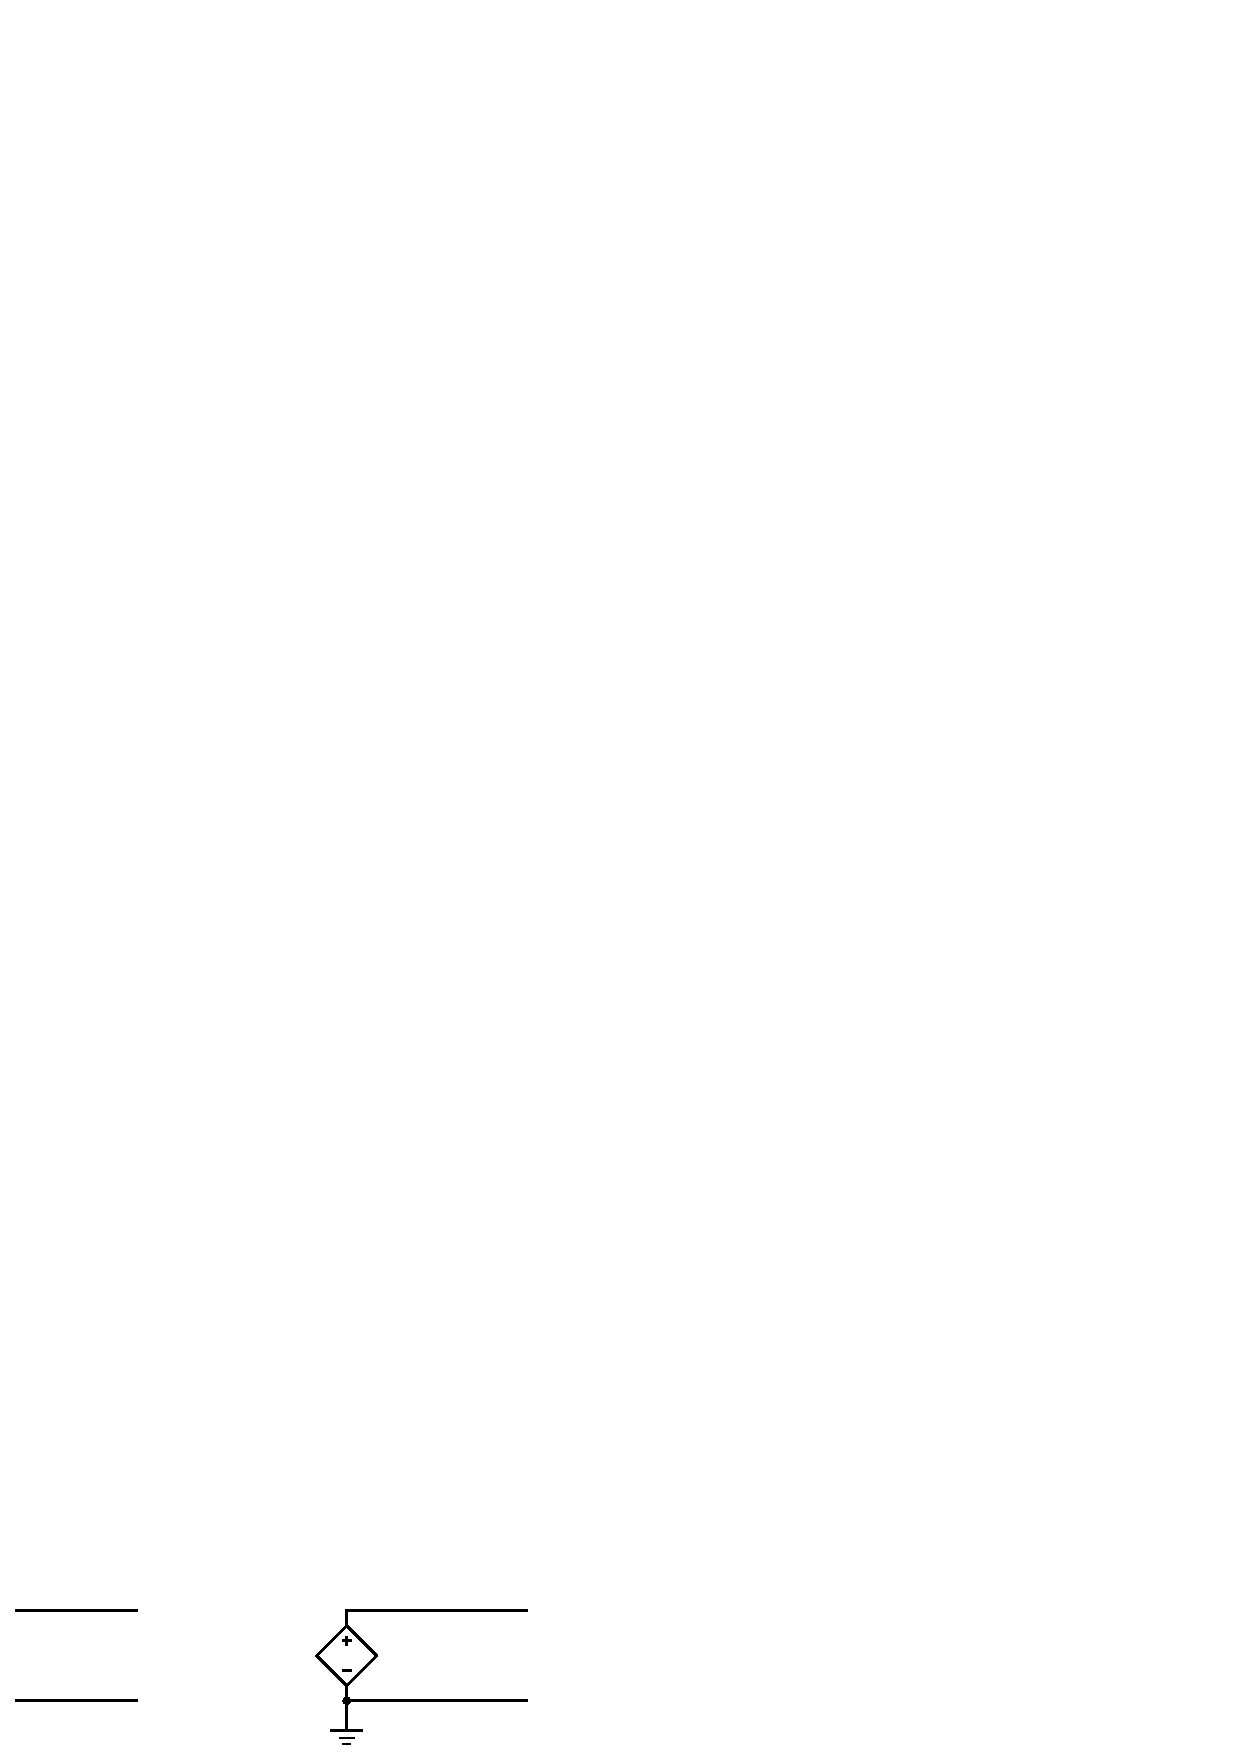
\includegraphics[scale=0.90]{idealOpampEquivalentCircuit}
\caption{کامل حسابی ایمپلیفائر کا مساوی دور}
\label{شکل_کامل_حسابی_ایمپلیفائر_کا_مساوی_دور}
\end{figure}
	اس شکل سے واضح ہے کہ داخلی سروں پر برقی رو صفر ایمپیئر ہے، داخلی مزاحمت لامحدود جبکہ خارجی مزاحمت صفر اُوہم ہے۔

\ابتدا{مثال}
\begin{itemize}
\item
جدول \حوالہ{جدول_حسابی_ایمپلیفائر_عمومی_مقداریں} میں دیے مقدار اور حسابی ایمپلیفائر کا غیر کامل مساوی دور استعمال کرتے ہوئے \عددی{v_s=\SI{1}{\volt}} پر  شکل \حوالہ{شکل_منفی_ایمپلیفائر} میں \عددی{v_o} کی قیمت حاصل کریں۔\عددی{R_1=\SI{1}{\kilo \ohm}} اور \عددی{R_1=\SI{10}{\kilo \ohm}} ہیں۔
\item
حسابی ایمپلیفائر کا کامل مساوی دور اور جدول \حوالہ{جدول_حسابی_ایمپلیفائر_عمومی_مقداریں} میں دیے گئے \عددی{A_d} کی قیمت استعمال کرتے ہوئے  دوبارہ  \عددی{v_o} کی قیمت حاصل کریں۔
\item
دونوں جوابات کا موازنہ کریں۔
\end{itemize}
%
\begin{figure}
\centering
\includegraphics[scale=0.90]{opampModelUsageExample}
\caption{حسابی ایمپلیفائر کے مساوی دور کا استعمال}
\label{شکل_حسابی_ماڈل_استعمال}
\end{figure}
%
حل:
شکل \حوالہ{شکل_حسابی_ماڈل_استعمال} الف میں حسابی ایمپلیفائر کا غیر کامل مساوی دور جبکہ شکل  الف     میں اس کا کامل مساوی دور استعمال کرتے ہوئے شکل \حوالہ{شکل_منفی_ایمپلیفائر} کو بنایا گیا ہے۔
\begin{itemize}
\item
شکل-الف میں کرچاف کے قانون برائے برقی رو استعمال کرتے ہوئے
\begin{align*}
\frac{v_1-v_s}{R_1}+\frac{v_1}{R_i}+\frac{v_1-v_o}{R_2}=0\\
\frac{v_o-v_1}{R_2}+\frac{v_o-A_d v_d}{R_o}=0
\end{align*}
حاصل ہوتا ہے۔دیے گئے قیمتیں استعمال کرتے ہوئے اور \عددی{v_1=-v_d} لکھ کر حل کرتے ہیں۔
\begin{align*}
\frac{-v_d-1}{\num{1000}}+\frac{-v_d}{\num{10e12}}+\frac{-v_d-v_o}{\num{10000}}=0\\
\frac{v_o+v_d}{\num{10000}}+\frac{v_o-\num{100000} v_d}{\num{100}}=0
\end{align*}
\عددی{\tfrac{v_d}{10^{12}}} کو نظر انداز کرتے ہوئے  حاصل ہوتا ہے۔
\begin{align*}
v_d=\frac{1+0.1 v_o}{1.1}\\
v_o=\frac{\num{10000001}}{101} v_d
\end{align*}
 اور یوں
\begin{align*}
v_o=\SI{-10.00111}{\volt  \volt}
\end{align*}
حاصل ہوتا ہے۔
\item
شکل \حوالہ{شکل_حسابی_ماڈل_استعمال} ب پر کرچاف کے قانون برائے برقی رو کے استعمال کرتے ہوئے حل کرتے ہیں۔
\begin{align*}
\frac{v_1-v_s}{R_1}+\frac{v_1-A_d v_d}{R_2}=0\\
\frac{-v_d-v_s}{R_1}+\frac{-v_d-A_d v_d}{R_2}=0\\
v_d=\frac{-v_s}{1+\frac{R_1}{R_2}\left(1+A_d \right)}
\end{align*}
اور یوں \عددی{v_o=A_d v_d} لکھتے ہوئے
\begin{align} \label{مساوات_حسابی_کامل_مثال_حل}
v_o=\frac{-A_d v_s}{1+\frac{R_1}{R_2}\left(1+A_d \right)}
\end{align}
یعنی
\begin{align*}
v_o=\frac{-\num{100000} v_s}{1+\frac{\num{1000}}{\num{10000}}\left(1+\num{100000} \right)}=\SI{-9.9989}{\volt\per \volt}
\end{align*}
حاصل ہوتا ہے۔
\item
پہلے جواب کی نسبت سے دیکھتے ہوئے دونوں جوابات میں صرف
\begin{align*}
\abs{\frac{-10.00111+9.9989}{10.00111}} \times 100=\SI{0.0221}{\percent}
\end{align*}
کا فرق ہے جو کہ قابل نظر انداز ہے۔یوں اس مثال میں غیر کامل اور کامل مساوی ادوار استعمال کرتے ہوئے یکساں جوابات حاصل ہوتے ہیں۔
\end{itemize}
\انتہا{مثال}

مساوات \حوالہ{مساوات_حسابی_کامل_مثال_حل} میں \عددی{A_d \gg 1} اور  \عددی{\tfrac{R_1}{R_2} \left(1+A_d \right) \gg 1} ہے۔
یوں اس مساوات کو با آسانی اس طرح بھی حل کیا جا سکتا ہے
\begin{align*}
v_o=\frac{-A_d v_s}{1+\frac{R_1}{R_2}\left(1+A_d \right)} \approx \frac{-A_d v_s}{\frac{R_1}{R_2}\left(1+A_d \right)}  \approx \frac{-A_d v_s}{\frac{R_1}{R_2}\left(A_d \right)} =-\frac{R_2}{R_1}v_s
\end{align*}

یہی جواب \عددی{A_d \gg 1} اور  \عددی{\tfrac{R_1}{R_2} \left(1+A_d \right) \gg 1} کے  حقائق (یا شرائط) کی بجائے  \عددی{A_d \to \infty} تصور کرتے ہوئے بھی حاصل  کیا جا سکتا تھا۔

اس مثال میں حسابی ایمپلیفائر کے ساتھ بیرونی جوڑے گئے مزاحمت \عددی{R_1} اور \عددی{R_2} کی قیمتیں حسابی ایمپلیفائر کے اندرونی مزاحمت \عددی{R_i} سے بہت کم اور اندرونی مزاحمت \عددی{R_o} سے بہت زیادہ تھیں۔مزید یہ کہ \عددی{A_d} کی قیمت کو لامحدود تصور کرتے ہوئے زیادہ آسانی سے جواب حاصل ہوتا ہے۔

جب بھی حسابی ایمپلیفائر کے ساتھ بیرونی جڑے مزاحمت کی قیمت \عددی{R_i} سے بہت کم اور \عددی{R_o} سے بہت زیادہ ہو، ایسی صورت میں غیر کامل اور کامل مساوی ادوار دونوں کے استعمال سے یکساں جوابات حاصل ہوتے ہیں۔چونکہ کامل دور استعمال کرتے ہوئے جواب زیادہ آسانی سے حاصل ہوتا ہے لہٰذا ایسی صورت میں کامل مساوی دور ہی استعمال کیا جاتا ہے۔مزید یہ کہ \عددی{A_d \to \infty} تصور کرنے سے مسئلہ حل کرنا نہایت آسان ہو جاتا ہے۔ان تین حقائق کو یہاں بیان کرتے ہیں۔
\begin{gather}
\begin{aligned} \label{مساوات_حسابی_کامل_دور_یقینی}
R_{\textup{بیرونی}}&<< R_i\\
R_{\textup{بیرونی}}&>> R_o\\
A_d & \to \infty
\end{aligned}
\end{gather}
حسابی ایمپلیفائر کے استعمال میں بیرونی مزاحمتوں کی قیمتیں تعین کرتے وقت اس بات کو یقینی بنایا جاتا ہے کہ یہ مساوات \حوالہ{مساوات_حسابی_کامل_دور_یقینی} پر پورا اتریں۔آئیں اب ایسے ادوار دیکھیں جو مساوات \حوالہ{مساوات_حسابی_کامل_دور_یقینی} پر پورا اترتے ہوں۔

\ابتدا{مثال}
شکل \حوالہ{شکل_منفی_ایمپلیفائر} میں حسابی ایمپلیفائر کا کامل مساوی دور استعمال کرتے ہوئے داخلی مزاحمت کی مساوات حاصل کریں۔

حل:
 شکل \حوالہ{شکل_حسابی_ماڈل_استعمال} ب  میں کامل دور استعمال کرتے ہوئے اسی کو دوبارہ دکھایا گیا ہے۔منفی داخلی سرے  پر کرچاف کے قانون برائے برقی رو استعمال کرتے ہوئے اس میں \عددی{v_o=A_d v_d} یعنی \عددی{v_o=-A_d v_1} ڈالتے ہیں۔
\begin{align*}
\frac{v_1-v_s}{R_1}+\frac{v_1-v_o}{R_2}=0\\
\frac{v_1-v_s}{R_1}+\frac{v_1+A_d v_1}{R_2}=0\\
v_1 =\left(\frac{1}{R_1}+\frac{1+A_d}{R_2} \right)=\frac{v_s}{R_1}\\
v_1=\frac{v_s}{R_1} \left(\frac{1}{\frac{1}{R_1}+\frac{1+A_d}{R_2} } \right)
\end{align*}
اس نتیجے کو استعمال کرتے ہوئے  \عددی{v_s} سے \عددی{v_1} کی جانب برقی رو \عددی{i_s} یوں حاصل ہو گی۔
\begin{align*}
i_s=\frac{v_s-v_1}{R_1} =\frac{v_s}{R_1} -\frac{v_s}{R_1^2} \left(\frac{1}{\frac{1}{R_1}+\frac{1+A_d}{R_2} } \right)
\end{align*} 
جس سے داخلی مزاحمت کی مساوات یوں حاصل ہوتی ہے۔
\begin{align}
R_{\textup{داخلی}}=\frac{v_s}{i_s}=R_1+\frac{R_2}{1+A_d}
\end{align}

\انتہا{مثال}

\حصہ{حسابی ایمپلیفائر کے ادوار} \label{حصہ_حسابی_ایمپلیفائر_کے_ادوار}

حسابی ایمپلیفائر کو استعمال کرتے خارجی اشارہ کا کچھ حصہ لے کر اسے دوبارہ داخلی اشارہ کے طور استعمال کیا جاتا ہے۔ایسے ادوار کو \موٹا{واپسی ادوار}  کہتے ہیں اور ایسے واپس کردہ اشارے کو \موٹا{واپسی اشارہ}\حاشیہب{feedback signal}  کہتے ہیں۔اس بات کی وضاحت جلد ہو گی۔

\جزوحصہ{منفی ایمپلیفائر}

	شکل \حوالہ{شکل_منفی_ایمپلیفائر} میں دکھائے دور کو مثال بناتے ہوئے ہم حسابی ایمپلیفائر پر مبنی ادوار حل کرنا سیکھتے ہیں۔اس دور کو \موٹا{منفی ایمپلیفائر}\فرہنگ{منفی ایمپلیفائر}\فرہنگ{amplifier!inverting}\حاشیہب{inverting amplifier}  کہتے ہیں۔
\begin{figure}
\centering
\includegraphics[scale=0.90]{invertingAmplifier}
\caption{منفی ایمپلیفائر}
\label{شکل_منفی_ایمپلیفائر}
\end{figure}
	اس شکل میں حسابی ایمپلیفائر کے داخلی سروں پر برقی دباو کو \عددی{v_k}  اور \عددی{v_n} جبکہ خارجی سرے پر برقی دباو کو \عددی{v_o} کہا گیا ہے۔اس کتاب میں یہی علامتیں استعمال کی جائیں گی۔

	ایسے  ادوار حل کرنے کی خاطر ہم حسابی ایمپلیفائر کے داخلی سروں پر \موٹا{کرچاف کے قوانین}\فرہنگ{کرچاف کے قوانین}\حاشیہب{Kirchoff's laws}  کا سہارا لیتے ہیں۔\موٹا{جوڑ}\فرہنگ{جوڑ}\حاشیہب{node}  \عددی{v_n} سے تین شاخیں نکلتی ہیں۔شکل میں ان شاخوں میں برقی رو کو \عددی{i_1} ، \عددی{i_2} اور \عددی{i_3} کہا گیا ہے۔\موٹا{کرچاف} کا قانون برائے برقی رو\حاشیہب{Kirchoff's current law}  کہتا ہے کہ کسی بھی جوڑ پر اندر کی جانب کل برقی رو اس جوڑ پر باہر کی جانب کل برقی رو کے برابر ہو گی۔چونکہ ہم نے جوڑ پر تمام برقی رو کو باہر کی جانب نکلتے تصور کیا ہے لہٰذا اس صورت میں ان کا مجموعہ صفر ہو گا یعنی
\begin{align} \label{مساوات_منفی_منفی_مداخل_کے_جوڑ_پر_رو}
i_1+i_2+i_3 = 0
\end{align}
مساوات \حوالہ{مساوات_حسابی_بنیادی_پہلو}  کے تحت حسابی ایمپلیفائر کے داخلی سرے پر برقی رو کی قیمت صفر ہوتی ہے ۔اس مثال میں اس برقی رو کو \عددی{i_3} کہا گیا ہے لہٰذا
\begin{align} \label{مساوات_حسابی_منفی_سرے_پر_صفر_رو}
i_3=0
\end{align}
ہے۔اُوہم کا قانون استعمال کرتے ہم \عددی{i_1} اور \عددی{i_2} حاصل کرتے ہیں۔
\begin{gather} 
\begin{aligned}\label{مساوات_منفی_بقایا_داخلی_رو}
i_1& =\frac{v_n-v_s}{R_1}\\
i_2 &=\frac{n_n-v_o}{R_2}
\end{aligned}
\end{gather}
مساوات \حوالہ{مساوات_حسابی_منفی_سرے_پر_صفر_رو}  اور \حوالہ{مساوات_منفی_بقایا_داخلی_رو}  کو مساوات \حوالہ{مساوات_منفی_منفی_مداخل_کے_جوڑ_پر_رو}  میں استعمال کرتے حاصل ہوتا ہے
\begin{align} \label{مساوات_منفی_کا_حصول}
\frac{v_n - v_s}{R_1}+\frac{v_n-v_o}{R_2}+0=0
\end{align}
	جوڑ \عددی{v_n} پر کرچاف کا قانون برائے برقی رو استعمال کرتے ہم نے مساوات \حوالہ{مساوات_منفی_کا_حصول}  حاصل کی۔اگر جوڑ \عددی{v_k} پر بھی برقی ارکان مثلاً مزاحمتیں یا برقی اشارات جڑے ہوتے، تب اس جوڑ کو بھی بالکل جوڑ \عددی{v_n} کی طرح حل کرتے۔موجودہ مثال میں ایسا نہیں۔جوڑ \عددی{v_k} \موٹا{برقی زمین}\فرہنگ{برقی!زمین}\حاشیہب{ground} کے ساتھ جڑا ہے اور یوں ہم اس جوڑ کے لئے لکھ سکتے ہیں
\begin{align} \label{مساوات_منفی_مثبت__زمین_پر}
v_k=0
\end{align}
	حسابی ایمپلیفائر کے دونوں داخلی برقی سروں والے جوڑوں کے لئے یوں مساواتیں حاصل کرنے کے بعد ہم مساوات \حوالہ{مساوات_حسابی_بنیادی_پہلو}  کی پہلی شِق استعمال کرتے ہیں۔مساوات \حوالہ{مساوات_منفی_مثبت__زمین_پر}  سے \عددی{v_k} کی قیمت کو مساوات \حوالہ{مساوات_منفی_کا_حصول}  میں \عددی{v_n} میں استعمال کرتے حل کرتے ہیں۔
\begin{align}
& \frac{0-v_s}{R_1}+\frac{0-v_o}{R_2}=0 \nonumber \\
& -\frac{v_s}{R_1}-\frac{v_o}{R_2}=0 \nonumber \\
& v_o =-\frac{R_2}{R_1} v_s
\end{align}
اس مساوات کو عموماً یوں لکھا جاتا ہے۔
\begin{align} \label{مساوات_منفی_افزائش}
A_v=\frac{v_o}{ v_s}=- \frac{R_2}{R_1}
\end{align}
	یہ مساوات شکل \حوالہ{شکل_منفی_ایمپلیفائر}  میں دیے \موٹا{منفی ایمپلیفائر} کے خارجی اشارہ \عددی{v_o}  اور مہیا کردہ داخلی اشارہ \عددی{v_s} کا تعلق بیان کرتا ہے۔اس مساوات میں \عددی{v_o} اور \عددی{v_s} کے کسر کو منفی ایمپلیفائر کے \موٹا{برقی دباو کی افزائش}\فرہنگ{افزائش!برقی دباو}\فرہنگ{voltage gain}\حاشیہب{voltage gain} \عددی{A_v} کہا گیا ہے۔اس اصطلاح کو عموماً چھوٹا کر کے \موٹا{منفی افزائش} یا صرف \موٹا{افزائش}\فرہنگ{افزائش}\فرہنگ{gain}\حاشیہب{gain} کہا جاتا ہے۔اس مساوات میں منفی کی علامت اس حقیقت کو بیان کرتا ہے کہ خارجی اور داخلی اشارے آپس میں \عددی{\SI{180}{\degree}} کے زاویہ پر ہیں۔

%=======================
\ابتدا{مثال}\شناخت{مثال_حسابی_غیر_خطی_کردار}
شکل \حوالہ{شکل_منفی_ایمپلیفائر} میں دکھلائے منفی ایمپلیفائر میں \عددی{R_1 = \SI{1}{\kilo \ohm}} اور \عددی{R_2 =\SI{10}{\kilo \ohm}} تصور کریں۔اس منفی ایمپلیفائر کو باری باری مندرجہ ذیل برقی اشارات بطور \عددی{v_s} مہیا کیا جاتا ہے۔ان تمام کے لئے حسابی دور کا خارجی اشارہ \عددی{v_o} حاصل کریں۔حل کرتے وقت \عددی{V_{CC}=\SI{+15}{\volt}} اور \عددی{V_{EE}=\SI{-15}{\volt}} تصور کریں۔
\begin{enumerate}
\item $\begin{aligned}[t]
v_s = \SI{0.2}{\volt}
\end{aligned}$
\item $\begin{aligned}[t]
v_s = \SI{0.31}{\volt}
\end{aligned}$

\item $\begin{aligned}[t]
v_s = \SI{-0.52}{\volt}
\end{aligned}$

\item $\begin{aligned}[t]
v_s = 0.1 \sin \left (t \right )
\end{aligned}$

\item $\begin{aligned}[t]
v_s = 2 \sin \left ( t \right )
\end{aligned}$
\end{enumerate}
حل:	جب تک خارجی اشارہ \عددی{v_o} مساوات \حوالہ{مساوات_حسابی_کے_خارجی_حدود}  میں دیے حدود کے اندر رہتا ہے، اس وقت تک مساوات \حوالہ{مساوات_منفی_افزائش}  منفی ایمپلیفائر کی خارجی اشارہ \عددی{v_o} حاصل کرنے کے لئے استعمال ہو گا یعنی
\begin{align*}
v_o = - \left ( \frac{R_2}{R_1} \right ) v_s = -\left ( \frac{10000}{1000} \right ) v_s=-10 v_s
\end{align*}
%
\begin{enumerate}
\item
$\begin{aligned}
v_o = -10 \times 0.2 = \SI{-2}{\volt}
\end{aligned}$

\item
$\begin{aligned}
v_o = -10 \times 0.31 = \SI{-3.1}{\volt}
\end{aligned}$

\item
$\begin{aligned}
v_o = -10 \times \left(-0.52 \right ) = \SI{5.2}{\volt}
\end{aligned}$

\item
$\begin{aligned}
v_o = -10 \times 0.1 \sin (t) = - \sin(t) 
\end{aligned}$

\item
$\begin{aligned}
v_o = -10 \times 2 \sin(t)=\underbrace{-20 \sin(t)}_{\text{غیر خطی خطہ}}
\end{aligned}$
\end{enumerate}

		اس مثال کی پہلی چار صورتوں میں مساوات \حوالہ{مساوات_منفی_افزائش}  سے صحیح جواب حاصل ہوتا ہے۔آخری صورت میں چونکہ حاصل \عددی{v_o} کی قیمت حسابی ایمپلیفائر کے خطی حدود سے تجاوز کرتی ہے لہٰذا اس جواب کو رد کیا جاتا ہے۔اس جواب کے نیچے غیر خطی خطہ لکھ کر اسی بات کی وضاحت کی گئی ہے۔اس صورت میں \عددی{t} کی قیمت تبدیل کرتے \عددی{v_o} کی قیمت \عددی{v_o = -20 \sin(t)} سے ہی حاصل کی جاتی ہے۔جب تک حاصل جواب مساوات \حوالہ{مساوات_حسابی_کے_خارجی_حدود}  میں دیے حدود کے اندر رہے اسے صحیح تصور کیا جاتا ہے۔جہاں \عددی{v_o}  کی قیمت \عددی{V_{CC}}سے بلند ہونے کی کوشش کرے وہاں \عددی{v_o=V_{CC}} لیا جاتا ہے۔اسی طرح جہاں \عددی{v_o} کی قیمت \عددی{V_{EE}} سے تجاوز کرے وہاں \عددی{v_o = V_{EE}} لیا جاتا ہے۔اس بات کی وضاحت شکل \حوالہ{شکل_حسابی_لبریز} میں کی گئی ہے۔اس شکل کی مدد سے آپ دیکھ سکتے ہیں کہ حسابی ایمپلیفائر \عددی{V_{EE}} تا \عددی{V_{CC}} کے حدود میں خطی رد عمل رکھتا ہے جبکہ ان حدود کے باہر یہ غیر خطی رد عمل رکھتا ہے جس سے خارجی اشارہ  تراشا جاتا ہے۔
\begin{figure}
\centering
\includegraphics[scale=0.90]{clippedSineWave}
\caption{حسابی ایمپلیفائر کے لبریز ہونے سے خارجی اشارہ  تراشا جاتا ہے}
\label{شکل_حسابی_لبریز}
\end{figure}
\انتہا{مثال}

%============

	اس مثال میں آپ نے دیکھا کہ \عددی{v_s} کے مثبت ہونے کی صورت میں\عددی{v_o} کی قیمت منفی ہوتی ہے جبکہ \عددی{v_s} کے منفی ہونے کی صورت میں \عددی{v_o}کی قیمت مثبت ہوتی ہے یعنی منفی ایمپلیفائر مہیا کردہ داخلی اشارے \عددی{v_s} کی قیمت کو اُلٹ کرتا ہے۔اسی لئے اسے \موٹا{منفی ایمپلیفائر}\حاشیہب{inverting amplifier}\فرہنگ{منفی ایمپلیفائر}\فرہنگ{amplifier!inverting}  کہا جاتا ہے۔

	اسی مثال میں آپ نے دیکھا کہ \عددی{v_o} کی قیمت \عددی{v_s} کے منفی دس \عددی{-10} گنا ہے یعنی یہ دور مہیا کردہ اشارہ کے حیطہ کو بڑھا کر خارج کرتا ہے۔اس مثال میں منفی ایمپلیفائر کی  برقی دباو کی افزائش کی قیمت \عددی{-10} ہے۔منفی ایمپلیفائر کی افزائش مساوات \حوالہ{مساوات_منفی_افزائش}  سے حاصل ہوتی ہے۔

\begin{figure}
\centering
\includegraphics[scale=0.90]{invertingAmplifierInputResistance}
\caption{منفی حسابی ایمپلیفائر کی داخلی مزاحمت}
\label{شکل_حسابی_منفی_داخلی_مزاحمت}
\end{figure}
\ابتدا{مثال} \شناخت{مثال_حسابی_خطی_غیر_خطی_خطے}
مثال \حوالہ{مثال_حسابی_غیر_خطی_کردار} کے پہلے اجزاء میں ایمپلیفائر خطی خطے میں رہتا ہے جبکہ آخری جزو میں یہ غیر خطی خطے میں داخل ہوتا ہے۔انہیں پر مزید غور کرتے ہیں۔\عددی{v_s=\SI{0.52}{\volt}} اور  \عددی{v_s=\SI{2}{\volt}} کی صورت میں \عددی{v_n} حاصل کریں۔

حل:
پہلی صورت میں \عددی{v_o=\SI{-5.2}{\volt}} اور دوسری صورت میں \عددی{v_o=\SI{-15}{\volt}} ہوں گے۔جوڑ \عددی{v_n} پر کرچاف کے قانون برائے برقی رو سے
\begin{align*}
\frac{v_n -v_s}{R_1}+\frac{v_n-v_o}{R_2}=0\\
v_n=\frac{v_s R_2+v_o R_1}{R_1+R_2}
\end{align*}
حاصل ہوتا ہے لہٰذا پہلی صورت میں \عددی{v_n=\SI{0}{\volt}} جبکہ دوسری صورت میں \قریب{\عددی{v_n=\SI{0.45}{\volt}}} ہوں گے۔دونوں صورتوں میں مثبت داخلی سرا برقی زمین کے ساتھ جڑا ہے لہٰذا \عددی{v_k=\SI{0}{\volt}} رہتا ہے۔

آپ دیکھ سکتے ہیں کہ جب تک ایمپلیفائر خطی خطے میں رہے \عددی{v_n=v_k} رہتا ہے جبکہ غیر خطی خطے میں داخل ہوتے ہی \عددی{v_n \ne v_k} ہو جاتا ہے۔
\begin{align}
v_d &=0   \hspace{5mm} \textrm{خطی خطہ}\\
v_d & \ne 0 \hspace{5mm} \textrm{غیر خطی خطہ}
\end{align}
\انتہا{مثال}

منفی حسابی ایمپلیفائر کا داخلی مزاحمت \سیدھازیرنوشت{R}{داخلی} حاصل کرنے کی خاطر شکل \حوالہ{شکل_حسابی_منفی_داخلی_مزاحمت} سے رجوع کریں۔داخلی مزاحمت حاصل کرنے کی خاطر دور پر \عددی{v_t} لاگو کرتے ہوئے \عددی{i_t} ناپا جاتا ہے۔ان دو مقداروں کی شرح  کو داخلی مزاحمت کہا جاتا ہے یعنی
\begin{align*}
R_{\textup{داخلی}}=\frac{v_t}{i_t}
\end{align*}
چونکہ جوڑ \عددی{v_k} برقی زمین کے ساتھ جڑا ہے لہٰذا \عددی{v_k=0} ہو گا اور یوں \عددی{v_n} بھی صفر وولٹ پر ہو گا۔اس طرح \عددی{R_1} کا دایاں سرا صفر وولٹ پر ہے جبکہ اس کے بائیں سرے پر \عددی{v_t} لاگو کیا گیا ہے لہٰذا \عددی{i_t=\tfrac{v_t}{R_1}} ہو گا۔اس قیمت کو مندرجہ بالا مساوات میں استعمال کرتے  ہوئے
\begin{align}
R_{\textup{داخلی}}=R_1
\end{align}
حاصل ہوتا ہے۔جیسا شکل میں دکھایا گیا ہے، مزاحمت \عددی{R_1} سے گزرتی برقی رو \عددی{i_t} جوڑ \عددی{v_n} پر صرف \عددی{R_2} کے جانب جا سکتی ہے۔یوں \عددی{R_2} میں بھی \عددی{i_t} برقی رو پائی جائے گی جس سے اس مزاحمت کے دو سروں کے درمیان \عددی{i_t R_2} برقی دباو پیدا ہو گا۔چونکہ \عددی{R_2} کا بایاں سرا صفر وولٹ پر ہے لہٰذا اس کا دایاں سرا یعنی جوڑ \عددی{v_o} پر \عددی{-i_t R_2} برقی دباو پایا جائے گا۔اس طرح
\begin{align*}
v_o=-i_t R_2 =-\frac{v_t}{R_1} R_2
\end{align*}
ہو گا جس سے منفی حسابی ایمپلیفائر کی جانی پہچانی مساوات
\begin{align}
A_v=\frac{v_o}{v_t}=-\frac{R_2}{R_1}
\end{align}
حاصل ہوتی ہے۔

منفی حسابی ایمپلیفائر کی افزائش برقرار رکھتے ہوئے اس کے داخلی مزاحمت کو بڑھانے کی خاطر \عددی{R_1} کی قیمت بڑھانی ہو گی۔چونکہ \عددی{A_v=-\tfrac{R_2}{R_1}} ہے لہٰذا \عددی{R_1} بڑھاتے وقت \عددی{R_2} کی قیمت بھی بڑھانی ہو گی۔کبھی کبھار \عددی{R_2} کی قیمت اتنی بڑھ جاتی ہے کہ اس سے دیگر مسائل پیدا ہوتے ہیں۔آئیں دیکھیں کہ ایسی صورت حال سے کیسے نپٹا جا سکتا ہے۔

\ابتدا{مثال} \شناخت{مثال_حسابی_منفی_زیادہ_داخلی_مزاحمت}
شکل \حوالہ{شکل_حسابی_منفی_داخلی_زیادہ_مزاحمت} میں دکھائے دور کی افزائش حاصل کریں۔

حل:
\عددی{v_k=0} کی وجہ سے \عددی{v_n=0} ہے لہٰذا \عددی{i_1=\tfrac{v_s}{R_1}} ہو گا۔\عددی{i_1} جوڑ \عددی{v_n} پر \عددی{R_2} کے جانب مڑ جائے گی۔یوں \عددی{i_2=i_1} ہو گا جس سے \عددی{v_1=-i_1 R_2} یعنی
\begin{align*}
v_1=-\frac{R_2}{R_1} v_s
\end{align*}
اور
\begin{align*}
i_3=\frac{0-v_1}{R_3}=\frac{R_2}{R_1 R_3} v_s
\end{align*}
ہوں گے۔\عددی{i_4=i_2+i_3} یعنی
\begin{align*}
i_4=\frac{v_s}{R_1}+\frac{R_2}{R_1 R_3} v_s=\left(1+\frac{R_2}{R_3} \right) \frac{v_s}{R_1}
\end{align*}
ہو گا جو مزاحمت \عددی{R_4} میں سے گزرتے ہوئے اس پر \عددی{i_4 R_4} برقی دباو پیدا کرے گا۔یوں
\begin{align*}
v_1-v_o=i_4 R_4=\left(1+\frac{R_2}{R_3} \right) \frac{R_4 v_s}{R_1}
\end{align*}
\عددی{v_1} کی قیمت کے استعمال سے
\begin{align*}
-\frac{R_2}{R_1} v_s-v_o=\left(1+\frac{R_2}{R_3} \right) \frac{R_4 v_s}{R_1}
\end{align*}
یعنی
\begin{align} \label{مساوات_حسابی_داخلی_مزاحمت_بڑھایا_گیا}
A_v=\frac{v_o}{v_s}=-\frac{R_2}{R_1}\left[1+\left(\frac{1}{R_2}+\frac{1}{R_3} \right)R_4 \right]
\end{align}
حاصل ہوتا ہے۔

\begin{figure}
\centering
\includegraphics[scale=0.90]{invertingAmplifierIncreasedInputResistance}
\caption{منفی حسابی ایمپلیفائر کا داخلی مزاحمت بڑھایا گیا ہے}
\label{شکل_حسابی_منفی_داخلی_زیادہ_مزاحمت}
\end{figure}

اس ایمپلیفائر کے داخلی مزاحمت کی قیمت \عددی{R_1} ہے۔
\انتہا{مثال}

اس مثال کے نتائج مد نظر رکھتے ہوئے ہم دیکھتے ہیں کہ داخلی مزاحمت بڑھانے کی خاطر اگر \عددی{R_1} کی قیمت بڑھائی جائے تو افزائش برقرار رکھنے کی خاطر یہ ضروری نہیں کہ \عددی{R_2}  کی قیمت بھی بڑھائی جائے۔ہم  \عددی{R_3} اور \عددی{R_4} کے قیمتیں ایسی رکھ سکتے ہیں کہ درکار افزائش حاصل کی جائے۔یہ بات خصوصی  طور پر غور طلب ہے کہ \عددی{R_3} کے قیمت کو کم کرتے ہوئے افزائش بڑھائی جا سکتی ہے لہٰذا \عددی{R_1} کی قیمت زیادہ سے زیادہ رکھتے ہوئے داخلی مزاحمت بڑھائی جا سکتی ہے۔ 

\ابتدا{مثال}
شکل \حوالہ{شکل_حسابی_منفی_داخلی_زیادہ_مزاحمت} میں داخلی مزاحمت \عددی{\SI{300}{\kilo \ohm}} جبکہ \عددی{A_v=\SI{-100}{\volt\per \volt}} درکار ہے۔ تمام مزاحمت حاصل کریں۔

حل:
داخلی مزاحمت  کی شرط کی وجہ سے \عددی{R_1=\SI{300}{\kilo \ohm}} رکھی جاتی ہے۔ ایسی صورت میں \عددی{R_2} اور \عددی{R_4} کو بھی \عددی{\SI{300}{\kilo \ohm}} ہی رکھتے ہوئے \عددی{R_3} کی قیمت مساوات  \حوالہ{مساوات_حسابی_داخلی_مزاحمت_بڑھایا_گیا} سے \عددی{\SI{3061}{\ohm}}حاصل ہوتی ہے۔  
\انتہا{مثال}
%=============

مزاحمت کو اس کے قیمت سے پکارا جاتا ہے۔یوں \عددی{\SI{1}{\kilo \ohm}} قیمت کے مزاحمت کو \عددی{\SI{1}{\kilo \ohm}} کا مزاحمت پکارا جائے گا۔\عددی{\SI{\mp 5}{\percent}} مزاحمت سے مراد ایسا مزاحمت ہے جس کی قیمت پکارے قیمت سے  پانچ فی صد زیادہ یا کم ممکن ہے۔یوں 
\عددی{\SI{1}{\kilo \ohm} \mp \SI{5}{\percent}} مزاحمت کی قیمت \عددی{\SI{0.95}{\kilo \ohm}} تا \عددی{\SI{1.05}{\kilo \ohm}} ممکن ہے۔\عددی{\SI{1}{\kilo \ohm}} کو مزاحمت کی \موٹا{پکاری گئی قیمت}\فرہنگ{پکاری گئی قیمت}\حاشیہب{nominal value} جبکہ  \عددی{\SI{\mp 5}{\percent}} کو قیمت میں \موٹا{غلطی}\فرہنگ{مزاحمت میں غلطی}\حاشیہب{tolerance} کہا جاتا ہے۔

مزاحمت \عددی{R} کی قیمت \عددی{\SI{5}{\percent}} بڑھنے سے \عددی{\tfrac{5}{100}R} بڑھ کر \عددی{\left(1+0.05 \right) R} ہو جائے گی۔اسی طرح \عددی{R} کی قیمت \عددی{\SI{5}{\percent}} کم ہونے سے  \عددی{\left(1-0.05 \right) R} ہو جائے گی۔ان دو قیمتوں کو ہم \عددی{\left(1+\epsilon \right)R} اور \عددی{\left(1-\epsilon \right)R} لکھ سکتے ہیں جہاں \عددی{\epsilon=0.05} کے برابر ہے۔

\ابتدا{مثال}
\موٹا{منفی حسابی ایمپلیفائر} میں \عددی{R_2=\SI{47}{\kilo \ohm}} جبکہ \عددی{R_1=\SI{1}{\kilo \ohm}} رکھا گیا۔دونوں مزاحمتوں کے قیمت میں \عددی{\SI{\mp 5}{\percent}} غلطی کی گنجائش ہے۔اس ایمپلیفائر کے ممکنہ افزائش کے حدود حاصل کریں۔

حل:منفی حسابی ایمپلیفائر کی افزائش \عددی{A= -\tfrac{R_2}{R_1}} کے برابر ہے۔اس کا حتمی قیمت اس وقت کم سے کم  ہو گا جب \عددی{R_2} کی حقیقی قیمت \عددی{\SI{5}{\percent}} کم یعنی \عددی{\left(1-\epsilon \right) R_2} جبکہ \عددی{R_1} کی حقیقی قیمت \عددی{\SI{5}{\percent}} زیادہ  یعنی \عددی{\left(1+\epsilon \right) R_2} ہو جہاں \عددی{\epsilon=0.05} کے برابر ہے۔اسی طرح افزائش کی زیادہ سے زیادہ قیمت اس وقت حاصل ہو گی جب \عددی{R_2} کی حقیقی قیمت \عددی{\SI{5}{\percent}} زیادہ جبکہ \عددی{R_1} کی حقیقی قیمت \عددی{\SI{5}{\percent}} کم ہو۔یوں
\begin{align*}
A_{\textrm{کمتر}}=-\frac{1-\epsilon}{1+\epsilon} \left(\frac{R_2}{R_1} \right)=-\frac{0.95}{1.05} \left(\frac{47000}{1000}\right)=-42.524\\
A_{\textrm{بلندتر}}=-\frac{1+\epsilon}{1-\epsilon} \left(\frac{R_2}{R_1} \right)=-\frac{1.05}{0.95} \left(\frac{47000}{1000}\right)=-51.947
\end{align*}
\انتہا{مثال}

اس مثال میں آپ نے دیکھا کہ مزاحمتوں کے قیمت میں \موٹا{غلطی کے گنجائش} کی وجہ سے افزائش کی قیمت درکار قیمت سے انحراف کر سکتی ہے۔موجودہ مثال میں ایمپلیفائر کے افزائش کی پکاری گئی قیمت \عددی{\SI{-47}{\volt \per \volt}} ہے جبکہ حقیقت میں یہ \عددی{\SI{-42.524}{\volt \per \volt}} تا \عددی{\SI{-51.947}{\volt \per \volt}} کے درمیان کہیں پر بھی ہو سکتی ہے۔یوں حقیقی افزائش، پکاری گئی قیمت سے
\begin{align*}
\abs{\frac{51.947-47}{47} \times 100} \approx \SI{10}{\percent}
\end{align*}
زیادہ یا کم ممکن ہے۔

%==================
\ابتدا{مثال}
شکل \حوالہ{شکل_حسابی_مزاحمت_نما_ایمپلیفائر} میں دکھائے دور کا داخلی مزاحمت، خارجی مزاحمت اور \موٹا{مزاحمت نما افزائش}\فرہنگ{مزاحمت نما افزائش}\حاشیہب{transconductance gain}\فرہنگ{transconductance gain} \عددی{R_m=\tfrac{v_o}{i_s}} حاصل کریں۔اس دور کو استعمال کرتے ہوئے برقی رو اشارے \عددی{i_s} سے برقی دباو کا اشارہ \عددی{v_o} حاصل کیا جاتا ہے۔ 
\begin{figure}
\centering
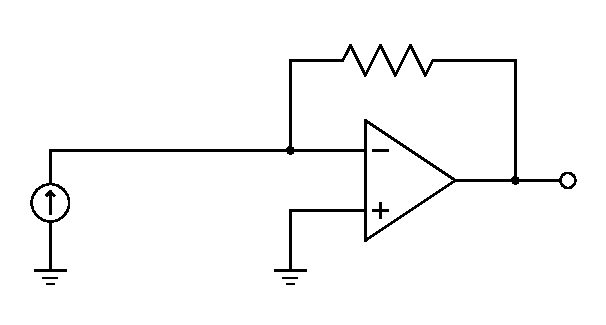
\includegraphics[scale=0.90]{opampTransconductanceAmplifier}
\caption{حسابی مزاحمت نما ایمپلیفائر}
\label{شکل_حسابی_مزاحمت_نما_ایمپلیفائر}
\end{figure}

حل:جوڑ \عددی{v_k} برقی زمین کے ساتھ جڑا ہے لہٰذا \عددی{v_k=0} اور یوں \عددی{v_n=0} ہو گا۔داخلی جانب برقی رو \عددی{i_s} جبکہ برقی دباو \عددی{v_n} ہے لہٰذا
\begin{align*}
R_{\textup{داخلی}}=\frac{v_n}{i_s}=\frac{0}{i_s}=\SI{0}{\ohm}
\end{align*}
حاصل ہوتا ہے۔

خارجی مزاحمت حاصل کرنے کی خاطر کامل حسابی ایمپلیفائر کا دور جسے شکل \حوالہ{شکل_کامل_حسابی_ایمپلیفائر_کا_مساوی_دور} میں دکھایا گیا ہے کو زیر استعمال لاتے ہیں۔\عددی{v_d=0} ہونے کی صورت میں اس کے خارجی جانب صفر اُوہم حاصل ہوتا ہے لہٰذا
\begin{align*}
R_{\textup{خارجی}}=\SI{0}{\ohm}
\end{align*}
حاصل ہوتا ہے۔

آئیں اب مزاحمت نما افزائش \عددی{R_m} حاصل کریں۔جیسے شکل میں دکھایا گیا ہے، جوڑ \عددی{v_n} پر آمد برقی رو \عددی{i_s} صرف مزاحمت \عددی{R} کی جانب جا سکتی ہے۔یوں اس مزاحمت پر \عددی{i_s R} برقی دباو پیدا ہو گا۔مزاحمت کا بایاں سرا برقی زمین پر ہے لہٰذا
\begin{align*}
v_o=-i_s R\\
R_m=\frac{v_o}{i_s}=-R
\end{align*}
ہو گا۔
\انتہا{مثال}

حسابی منفی ایمپلیفائر کو شکل \حوالہ{شکل_حسابی_واپسی_منفی_ایمپلیفائر} الف میں دوبارہ دکھایا گیا ہے جبکہ شکل  الف     میں اسی کو قدر مختلف طرز پر بنایا گیا ہے۔شکل  الف     میں یہ بات کھل کر سامنے آتی ہے کہ خارجی اشارہ \عددی{v_o} کو بھی بطور داخلی اشارہ استعمال کیا جا رہا ہے۔
\begin{figure}
\centering
\includegraphics[scale=0.90]{feedbackInvertingAmplifier}
\caption{واپسی حسابی منفی ایمپلیفائر}
\label{شکل_حسابی_واپسی_منفی_ایمپلیفائر}
\end{figure}

ایسے ادوار جن میں خارجی اشارہ کو بطور داخلی اشارہ استعمال کیا گیا ہو کو \موٹا{واپسی ادوار}\فرہنگ{واپسی ادوار}\حاشیہب{feedback circuits} کہتے ہیں اور جن خارجی  اشارات کو یوں بطور داخلی اشارات استعمال کیا گیا ہو انہیں \موٹا{واپسی اشارات}\فرہنگ{واپسی اشارات}\حاشیہب{feedback signals}\فرہنگ{feedback signal}  کہتے ہیں۔یوں منفی ایمپلیفائر \موٹا{واپسی ادوار} کی ایک مثال ہے۔

حسابی ایمپلیفائر کے تفرقی افزائش برقی دباو \عددی{A_d}  کی قیمت لامحدود ہونے کے وجہ سے نہایت کم داخلی اشارے پر بھی اس کو غیر خطی خطے میں داخل ہونا چاہیے۔حقیقت میں ایمپلیفائر استعمال ہی خطی خطے میں ہوتا ہے اور واپسی اشارے کی شمولیت اس کو ممکن بناتی ہے۔

حسابی منفی ایمپلیفائر پر دوبارہ غور کریں۔داخلی اشارہ \عددی{v_s} کو منفی داخلی سرے پر مہیا کیا گیا ہے۔جیسا شکل میں تیر کے نشانوں سے دکھایا گیا ہے کہ اگر داخلی اشارہ \عددی{v_s} کو مثبت جانب \عددی{(\uparrow)} لے جایا جائے تو خارجی اشارہ \عددی{v_o} منفی جانب \عددی{(\downarrow)} حرکت کرتا ہے۔ اسی طرح اگر داخلی اشارہ \عددی{v_s} کو منفی جانب \عددی{(\downarrow)} لے جایا جائے تو خارجی اشارہ \عددی{v_o} مثبت جانب  حرکت کرتا ہے۔منفی داخلی سرے  پر کرچاف کے قانون برائے برقی رو سے 
\begin{align}\label{مساوات_حسابی_واپسی_منفی}
\frac{v_n-v_s}{R_1}+\frac{v_n-v_o}{R_2}=0\\
v_0=\frac{R_2}{R_1} v_s
\end{align}
حاصل ہوتا ہے جہاں  دوسرے قدم پر \عددی{v_k=0} کی وجہ سے \عددی{v_n=0} کا استعمال کیا گیا۔اسی حقیقت کو یوں بھی دیکھا جا سکتا ہے کہ حسابی ایمپلیفائر \عددی{v_o} کو یوں رکھتا ہے کہ \عددی{v_d=0} یعنی \عددی{v_k=v_n}  حاصل ہو۔چونکہ منفی حسابی ایمپلیفائر میں \عددی{v_k=0} ہے لہٰذا حسابی ایمپلیفائر \عددی{v_o} کو یوں رکھے گا کہ \عددی{v_n=0} حاصل ہو۔شکل \حوالہ{شکل_حسابی_واپسی_منفی_ایمپلیفائر} پ میں \عددی{v_n} کی مساوات حاصل کرتے ہوئے  اس مساوات پر \عددی{v_n=0} کی شرط لاگو کریں۔ایسا کرنے سے مساوات \حوالہ{مساوات_حسابی_واپسی_منفی} ہی حاصل ہوتے ہیں۔
%---------------------
\ابتدا{مثال}
حسابی منفی ایمپلیفائر میں \عددیء{R_1=\SI{1}{\kilo \ohm}}، \عددیء{R_2=\SI{5}{\kilo \ohm}} لیتے ہوئے \عددیء{v_s=\SI{1}{\volt}}، \عددیء{v_s=\SI{1.5}{\volt}}  اور \عددیء{v_s=\SI{2}{\volt}}  پر \عددی{v_o} حاصل کریں۔تینوں جوابات کو استعمال کرتے ہوئے شکل \حوالہ{شکل_حسابی_واپسی_منفی_ایمپلیفائر} پ میں \عددی{v_n} کی قیمت حاصل کریں۔

حل:
ان داخلی اشارات پر
\begin{align*}
v_o&=-\left(\frac{5000}{1000}\right) \times 1=\SI{-5}{\volt}\\
 v_o&=-\left(\frac{5000}{1000}\right) \times 1.5=\SI{-7.5}{\volt}\\
v_o&=-\left(\frac{5000}{1000}\right) \times 2=\SI{-10}{\volt}
\end{align*}
حاصل ہوتے ہیں۔آئیں ہر داخلی-خارجی برقی دباو کے جوڑے کو استعمال کرتے ہوئے شکل \حوالہ{شکل_حسابی_واپسی_منفی_ایمپلیفائر} پ میں \عددی{v_n} حاصل کریں۔کرچاف کے قانون برائے برقی رو سے
\begin{align*}
\frac{v_n-v_s}{R_1}+\frac{v_n-v_o}{R_2}=0\\
v_n=\frac{R_2 v_s +R_1 v_o}{R_1+R_2}
\end{align*}
حاصل ہوتا ہے اور یوں
\begin{align*}
v_n&=\frac{5000 \times 1 +1000 \times (-5)}{1000+5000}=\SI{0}{\volt}\\
v_n&=\frac{5000 \times 1.5 +1000 \times (-7.5)}{1000+5000}=\SI{0}{\volt}\\
v_n&=\frac{5000 \times 2 +1000 \times (-10)}{1000+5000}=\SI{0}{\volt}
\end{align*}
حاصل ہوتے ہیں۔
\انتہا{مثال}

مندرجہ بالا مثال میں ہم نے دیکھا کہ \عددی{v_o} اس جانب حرکت کرتا ہے جس جانب \عددی{v_k-v_n} یعنی \عددی{v_d} کی قیمت صفر حاصل ہو۔وہ واپسی دور جس کا خارجی اشارہ، دور کے داخلی اشارے کے الٹ کام کرے کو \موٹا{منفی واپسی دور}\فرہنگ{منفی واپسی دور}\فرہنگ{feedback circuit!negative}\حاشیہب{negative feedback circuit} کہتے ہیں اور اس عمل کو \موٹا{منفی واپسی عمل} یا صرف \موٹا{منفی واپسی} کہتے ہیں۔اس باب میں \موٹا{منفی واپسی ادوار} حل کرنے پر غور کیا جائے گا۔\موٹا{مثبت واپسی} کا استعمال باب \حوالہ{باب_مرتعش} میں دیکھا جائے گا۔  
 
شکل \حوالہ{شکل_حسابی_مثبت_واپسی_دور} میں  \موٹا{مثبت واپسی دور} کی مثال دکھائی گئی ہے۔یہاں \عددی{v_s} حسابی ایمپلیفائر کے مثبت داخلی سرے  پر مہیا کیا گیا ہے۔یوں \عددی{v_s} بڑھانے سے \عددی{v_d} بڑھے گا اور یوں \عددی{v_o} بھی مثبت جانب بڑھے گا۔جیسے شکل  الف     میں دکھایا گیا ہے کہ \عددی{v_s} اور \عددی{v_o} دونوں بڑھنے سے \عددی{v_k} صرف بڑھ ہی سکتا ہے۔اگر \عددی{v_o} کو بطور واپسی اشارہ داخلی سرے  پر مہیا نہ کیا جاتا تب بھی \عددی{v_s} بڑھانے سے  \عددی{v_k} اور \عددی{v_d}بڑھتے لیکن \عددی{v_o} کا بطور واپسی اشارہ استعمال کرنے کی وجہ سے \عددی{v_k}   اور  \عددی{v_d} مزید زیادہ بڑھتے ہیں۔ایسے ادوار جن میں واپسی اشارہ اور داخلی اشارہ ایک ہی جانب کو حرکت کریں کو \موٹا{مثبت واپسی ادوار}\فرہنگ{مثبت واپسی ادوار}\فرہنگ{feedback circuit!positive}\حاشیہب{positive feedback circuit} کہتے ہیں۔ \موٹا{مثبت واپسی ادوار} کا خارجی اشارہ  عموماً مکمل مثبت یا مکمل منفی جانب غیر خطی خطے میں رہتا ہے ما سوائے ان لمحات کے جب یہ منفی سے مثبت یا مثبت سے منفی جانب حرکت کر رہا ہو۔
\begin{figure}
\centering
\includegraphics[scale=0.90]{feedbackPositiveOpampExplanation}
\caption{مثبت واپسی دور کی مثال}
\label{شکل_حسابی_مثبت_واپسی_دور}
\end{figure}
آئیں شکل \حوالہ{شکل_حسابی_مثبت_واپسی_دور} کو مثال بناتے ہوئے \موٹا{مثبت واپسی ادوار} حل کرنا دیکھتے ہیں۔تصور کریں کہ \عددی{v_s=0} اور \عددی{v_o=0} صفر ہیں۔یوں شکل  الف     میں 
\begin{align*}
v_k=\frac{R_2 v_s+R_1 v_o}{R_1+R_2}=0
\end{align*}
حاصل ہوتا ہے۔یوں \عددی{v_d=v_k-v_n} بھی صفر رہے گا۔جیسا کہ ہم اب دیکھیں گے کہ اس حال میں مثبت واپسی دور نہایت غیر مستحکم حال میں ہے۔تصور کریں کہ کسی وجہ سے \عددی{v_s} کی قیمت بڑھ کر \عددی{v_s=\Delta v} ہو جاتی ہے۔حسابی ایمپلیفائر کے رد عمل سے پہلے \عددی{v_o=0} ہی رہے گا اور یوں
\begin{align*}
v_k=\frac{R_2 \times \Delta v+R_1 \times  0}{R_1+R_2}=\left(\frac{R_2}{R_1+R_2}\right) \Delta v \\
v_d=v_k-v_n=\left(\frac{R_2}{R_1+R_2}\right) \Delta v 
\end{align*}
ہوں گے۔حسابی ایمپلیفائر \عددی{v_d} کو \عددی{A_d} گنا بڑھانا چاہے گا۔آئیں \عددی{v_o} کے بڑھنے کے عمل کو دیکھیں۔تصور کریں کہ خارجی اشارہ  بڑھتے بڑھتے \عددی{v_o=\Delta v_{o1}} ہو جاتا ہے۔اس طرح 
\begin{align*}
v_k=\frac{R_2 \times \Delta v+R_1 \times  \Delta v_{o1}}{R_1+R_2}=v_d
\end{align*}
ہو جائے گا۔جیسا کہ آپ دیکھ سکتے ہیں \عددی{v_d} کی قیمت پہلے سے بڑھ گئی ہے۔یوں \عددی{v_o} مزید بڑھے گا جس سے \عددی{v_d} مزید بڑھے گا۔آخر کار \عددی{v_o} مثبت سپلائی پر رکھ جائے گا یعنی \عددی{v_o=V_{CC}} ہو جائے گا۔اس وقت
\begin{align*}
v_k=\frac{R_2 \times \Delta v+R_1 \times  V_{CC}}{R_1+R_2} \approx \left(\frac{R_1}{R_1+R_2} \right) V_{CC}=v_d
\end{align*}
ہو گا۔آپ دیکھ سکتے ہیں کہ مثبت واپسی دور میں 
\begin{align}
v_k \ne v_n
\end{align}
ہوتے ہیں۔اسی وجہ سے \موٹا{مثبت ادوار} کو اس باب میں استعمال ہونے والے طریقے سے حل نہیں کیا جا سکتا جہاں ہم \عددی{v_k} اور \عددی{v_n} کے مساوات حاصل کرتے ہوئے  \عددی{v_k=v_n} تصور کر کے \عددی{v_o} کے لئے حل کرتے ہیں۔

\موٹا{مثبت واپسی دور} کی پہچان یہ ہے کہ اس کا خارجی اشارہ جب بھی حرکت کرے تو یہ اسی جانب حرکت کرتا ہے جس جانب دور کا داخلی اشارہ (بغیر واپس آئے) حرکت کرے۔

\ابتدا{مثال}
شکل \حوالہ{شکل_حسابی_مثبت_واپسی_دور} میں 
\begin{align*}
R_1=\SI{1}{\kilo \ohm} \hspace{5mm} R_2=\SI{9}{\kilo \ohm} \hspace{5mm} V_{CC}=\SI{12}{\volt} \hspace{5mm} V_{EE}=\SI{-12}{\volt}
\end{align*}
لیتے ہوئے \عددی{v_s} کی وہ قیمت حاصل کریں جس پر خارجی اشارہ مکمل منفی  سے مکمل مثبت جانب حرکت کرے گا۔ اسی طرح \عددی{v_s} کی وہ قیمت حاصل کریں جس پر خارجی اشارہ مکمل مثبت  سے مکمل منفی جانب حرکت کرے گا۔

حل:
تصور کریں کہ خارجی اشارہ مکمل منفی جانب ہے یعنی \عددی{v_o=\SI{-12}{\volt}} جبکہ \عددی{v_s=0} ہے۔اس وقت
\begin{align*}
v_k=v_d=\frac{9000 \times 0+1000 \times  12}{1000+9000}=\SI{1.2}{\volt}
\end{align*}
ہو گا۔\عددی{v_o} اس لمحہ منفی جانب حرکت کرے گا جب \عددی{v_d} کی قیمت منفی ہو جائے۔آئیں \عددی{v_d=0} پر درکار \عددی{v_s} کی قیمت حاصل کریں۔
\begin{align*}
0=\frac{9000 \times v_s+1000 \times  12}{1000+9000}\\
v_s=\SI{-1.333}{\volt}
\end{align*}
حاصل ہوتا ہے۔جوں ہی \عددی{v_s} کی قیمت \SI{-1.333}{\volt} سے کم ہو جائے، اسی لمحہ \عددی{v_o=\SI{-12}{\volt}} ہو جائے گا۔

اسی طرح اگر \عددی{v_o=\SI{-12}{\volt}} ہے  تو خارجی اشارہ اس وقت مثبت جانب حرکت کرے گا جب
\begin{align*}
0=\frac{9000 \times v_s+1000 \times  \left(-12\right)}{1000+9000}\\
v_s=\SI{1.333}{\volt}
\end{align*}
\عددی{v_s>\SI{1.333}{\volt}} ہو۔
\انتہا{مثال}
%================

شکل \حوالہ{شکل_حسابی_زنجیری} میں دو منفی حسابی ایمپلیفائر سلسلہ وار جوڑتے ہوئے زنجیری ایمپلیفائر حاصل کیا گیا ہے۔زنجیر کے پہلی کڑی کا داخلی اشارہ \عددی{v_{s1}} جبکہ اس کا خارجی اشارہ  \عددی{v_{o1}} اور اس کی افزائش \عددی{A_{v1}=-\tfrac{R_2}{R_1}} ہے۔زنجیر کے دوسری کڑی کا داخلی اشارہ  \عددی{v_{s2}} جبکہ اس کا خارجی اشارہ  \عددی{v_{o2}} اور اس کی افزائش \عددی{A_{v2}=-\tfrac{R_4}{R_3}} ہے۔پہلے کڑی کے خارجی اشارے کو دوسرے کڑی کو بطور داخلی اشارہ مہیا کیا گیا ہے لہٰذا \عددی{v_{s2}=v_{o1}} ہے۔یوں ہم لکھ سکتے ہیں۔
\begin{align*}
v_{o1}&=A_{v1} v_{s1}
\end{align*}
اور
\begin{align*}
v_{o2}&=A_{v2} v_{s2}\\
&=A_{v2} v_{o1}
\end{align*}
اس مساوات میں گزشتہ مساوات سے حاصل \عددی{v_{o1}} استعمال کرتے ہوئے
\begin{align*}
v_{o2}=A_{v2} A_{v1} v_{s1}
\end{align*}
لکھا جا سکتا ہے۔زنجیری ایمپلیفائر کا داخلی اشارہ \عددی{v_{s1}} جبکہ اس کا خارجی اشارہ \عددی{v_{o2}} ہے۔یوں زنجیری ایمپلیفائر کی افزائش \عددی{A_{v}=\tfrac{v_{o2}}{v_{s1}}} کو مندرجہ بالا مساوات سے یوں حاصل کر سکتے ہیں۔
\begin{align}
A_v=\frac{v_{o2}}{v_{s1}}=A_{v1} A_{v2}
\end{align}

یہ ایک اہم نتیجہ ہے جس کے مطابق ایمپلیفائر سلسلہ وار جوڑنے سے ان کی افزائش آپس میں ضرب ہوتی ہے۔زنجری ایمپلیفائر میں مزید کڑیاں اسی طرح سلسلہ وار جوڑی جا سکتی ہیں۔
\begin{figure}
\centering
\includegraphics[scale=0.90]{cascadedOpampAmplifiers}
\caption{زنجیری حسابی ایمپلیفائر}
\label{شکل_حسابی_زنجیری}
\end{figure}

\جزوحصہ{مثبت ایمپلیفائر}

	شکل \حوالہ{شکل_مثبت_ایمپلیفائر}  میں ایک اور واپسی دور دکھایا گیا ہے جسے \موٹا{مثبت ایمپلیفائر}\فرہنگ{مثبت ایمپلیفائر}
\فرہنگ{amplifier!non-inverting}\حاشیہب{non-inverting amplifier}  کہتے ہیں۔آئیں اس دور کو کرچاف کے قوانین کی مدد سے حل کرتے ہیں۔
\begin{figure}
\centering
\includegraphics[scale=0.90]{nonInvertingAmplifier}
\caption{مثبت ایمپلیفائر}
\label{شکل_مثبت_ایمپلیفائر}
\end{figure}
	اس شکل میں جوڑ \عددی{v_n} سے باہر کی جانب تین برقی رو \عددیء{i_1}،\عددی{i_2} اور\عددی{i_3} نکلتے دکھائے گئے ہیں۔\عددی{i_3}چونکہ حسابی ایمپلیفائر کے داخلی سرے پر اندر کی جانب جاتی برقی رو ہے لہٰذا یہ مساوات \حوالہ{مساوات_حسابی_بنیادی_پہلو} کے شِق نمبر دو کی وجہ سے صفر کے برابر ہے۔باقی دو برقی رو کو اُوہم کے قانون کی مدد سے حاصل کیا جاتا ہے۔یوں
\begin{gather} 
\begin{aligned}\label{مساوات_مثبت_داخلی_سرے_پر_رو}
i_1 &=\frac{v_n}{R_1}\\
i_2&=\frac{v_n-v_o}{R_2}\\
i_3&=0
\end{aligned}
\end{gather}
جوڑ \عددی{v_k} چونکہ سیدھا فراہم کردہ برقی اشارہ \عددی{v_s} کے ساتھ جڑا ہے لہٰذا اس کے لئے ہم لکھ سکتے ہیں
\begin{align} \label{مساوات_مثبت_داخلی_دباو_اشارے_کے_برابر}
v_k = v_s
\end{align}
	کرچاف کے قانون برائے برقی رو کو مساوات \حوالہ{مساوات_مثبت_داخلی_سرے_پر_رو}  کے ساتھ مل کر استعمال کرتے حاصل ہوتا ہے
\begin{align} \label{مساوات_مثبت_افزائش_کا_حصول}
&i_1+i_2+i_3=0 \nonumber\\
&\frac{v_n}{R_1}+\frac{v_n-v_o}{R_2}+0=0
\end{align}
مساوات \حوالہ{مساوات_حسابی_بنیادی_پہلو} کی پہلی شق کے مطابق \عددی{v_k}  اور \عددی{v_n} کی قیمتیں برابر رہتی ہیں۔یوں مساوات \حوالہ{مساوات_مثبت_داخلی_دباو_اشارے_کے_برابر}  میں دیے \عددی{v_k} کی قیمت کو مساوات \حوالہ{مساوات_مثبت_افزائش_کا_حصول}  میں \عددی{v_n} کی جگہ استعمال کرتے ہم مساوات \حوالہ{مساوات_مثبت_افزائش_کا_حصول}  کو حل کرتے ہیں۔
\begin{align}
\frac{v_s}{R_1}+\frac{v_s-v_o}{R_2} &=0 \nonumber \\
\frac{v_s}{R_1}+\frac{v_s}{R_2}-\frac{v_o}{R_2}&=0 \nonumber \\
\left (  \frac{v_s}{R_1} +\frac{v_s}{R_2}\right ) R_2 &=v_o \nonumber \\
\left(1+\frac{R_2}{R_1} \right )v_s &=v_o
\end{align}
اس مساوات کو عموماً یوں لکھا جاتا ہے۔
\begin{align} \label{مساوات_مثبت_افزائش}
A_v=\frac{v_o}{v_s}=\left(1+\frac{R_2}{R_1} \right )
\end{align}
\عددی{v_o} اور \عددی{v_s} کے کسر کو \موٹا{مثبت ایمپلیفائر} کی \موٹا{برقی دباو کی افزائش}\فرہنگ{افزائش!برقی دباو}\حاشیہب{voltage gain}\فرہنگ{voltage gain} \عددی{A_v} کہتے ہیں۔اس اصطلاح کو عموماً چھوٹا کر کے اسے صرف \موٹا{مثبت افزائش} کہتے ہیں۔

اس ایمپلیفائر کا داخلی مزاحمت حاصل کرنے کی خاطر \عددی{v_s} لاگو کرتے ہوئے \عددی{i_s} ناپتے ہیں۔چونکہ حسابی ایمپلیفائر کا داخلی برقی رو صفر ہوتا ہے لہٰذا \عددی{i_s=0} ہو گا۔یوں 
\begin{align}
R_{\textup{داخلی}}=\frac{v_s}{i_s}=\frac{v_s}{0} \to \infty
\end{align}
حاصل ہوتا ہے۔
%==============
\ابتدا{مثال}
شکل \حوالہ{شکل_مثبت_ایمپلیفائر} میں دکھلائے مثبت ایمپلیفائر میں \عددی{R_1 = \SI{2}{\kilo \ohm}} اور \mbox{\عددی{R_2=\SI{15}{\kilo \ohm}}} تصور کریں۔اس مثبت ایمپلیفائر کو باری باری مندرجہ ذیل برقی اشارات بطور \عددی{v_s} مہیا کیا جاتا ہے۔ان تمام کے لئے حسابی دور کا خارجی اشارہ \عددی{v_o} حاصل کریں۔حل کرتے وقت \عددی{V_{CC}=\SI{+15}{\volt}}  اور  \عددی{V_{EE}=\SI{-15}{\volt}} تصور کریں۔
\begin{enumerate}
\item 
$ \begin{aligned}
v_s = \SI{1.2}{\volt}
\end{aligned} $

\item 
$ \begin{aligned}
v_s = \SI{-0.25}{\volt}
\end{aligned} $

\item 
$ \begin{aligned}
v_s = 0.33 \cos (\omega t)
\end{aligned} $
\end{enumerate}
حل:	مساوات  \حوالہ{مساوات_مثبت_افزائش} سے اس مثبت ایمپلیفائر کی افزائش حاصل کرتے ہیں۔
\begin{align*}
A_v = \left (1+\frac{15000}{2} \right )=\SI{8.5}{\volt \per \volt}
\end{align*}
یوں
\begin{enumerate}
\item
$\begin{aligned}
v_o=A_v \times v_s = 8.5 \times 1.2=\SI{10.2}{\volt}
\end{aligned}$

\item
$\begin{aligned}
v_o=A_v \times v_s = 8.5 \times (-0.25)=\SI{2.125}{\volt}
\end{aligned}$

\item
$\begin{aligned}
v_o=A_v \times v_s = 8.5 \times 0.33 \cos (\omega t)=2.805 \cos (\omega t)
\end{aligned}$
\end{enumerate}
\انتہا{مثال}

%============

	اس مثال میں داخلی اشارہ مثبت ہونے کی صورت میں خارجی اشارہ  مثبت ہے جبکہ داخلی اشارہ منفی ہونے کی صورت میں خارجی اشارہ بھی منفی ہے۔یوں مثبت ایمپلیفائر داخلی اشارہ کو بغیر الٹائے بڑھا کر خارج کرتا ہے۔اسی لئے اسے \موٹا{مثبت ایمپلیفائر}\فرہنگ{مثبت ایمپلیفائر}\فرہنگ{amplifier!non-inverting}\حاشیہب{non-inverting amplifier}  کہتے ہیں۔

\جزوحصہ{مستحکم کار}

	مثبت ایمپلیفائر کی افزائش یہاں دوبارہ پیش کرتے ہیں۔
\begin{align}
A_v=1+\frac{R_2}{R_1}
\end{align}
اگر مثبت ایمپلیفائر میں \عددی{R_1} کی قیمت لامحدود لی جائے اور \عددی{R_2} کی قیمت صفر اُوہم  لی جائے تو اس مساوات کے مطابق اس کی افزائش
\begin{align}
A_v=1+\frac{0}{\infty} =1
\end{align}
ہو گی۔ایسا دور جسے \موٹا{مستحکم کار}\فرہنگ{مستحکم کار}\فرہنگ{buffer}\حاشیہب{buffer}  کہتے ہیں کو شکل \حوالہ{شکل_وسطی_دور} میں دکھایا گیا ہے۔اس دور کی افزائش ایک کے برابر جبکہ داخلی مزاحمت لامحدود ہے۔
\begin{figure}
\centering
\includegraphics[scale=0.90]{opampBuffer}
\caption{مستحکم کار}
\label{شکل_وسطی_دور}
\end{figure}
اس دور کو یوں بھی سمجھا جا سکتا ہے کہ مثبت داخلی سرے پر برقی دباو \عددی{v_s} ہے۔یوں منفی داخلی سرے پر  بھی اتنا ہی برقی دباو ہو گا مگر یہ سرا اور خارجی سرا آپس میں جڑے ہیں۔یوں خارجی سرے پر بھی یہی برقی دباو ہو گا یعنی \عددی{v_o = v_s} ہو گا جس سے افزائش \عددی{\tfrac{v_o}{v_s}=1} حاصل ہوتی ہے۔آئیں \موٹا{مستحکم کار} کا استعمال جانیں۔ 

طبعی متغیرات\حاشیہب{variables} مثلاً  کمیت، حرارت وغیرہ  کی برقیاتی پیمائش سے پہلے انہیں عموماً  \موٹا{مبدل توانائی}\فرہنگ{مبدل توانائی}\فرہنگ{transducer}\حاشیہب{transducer}  کے مدد سے برقی اشارات میں تبدیل کیا جاتا ہے اور ان برقی اشارات کو پیمایشی آلہ\فرہنگ{پیمایشی آلہ}\حاشیہب{measuring instrument}  سے ناپا جاتا ہے۔

	جیسا کہ آپ جانتے ہیں کہ کسی بھی دور کا تھونن  مساوی دور\فرہنگ{تھونن دور}\حاشیہب{Thevenin circuit} بنایا جا سکتا ہے جسے ایک عدد پیدا کار برقی دباو اور ایک عدد مزاحمت کی شکل دی جاتی ہے۔مبدل توانائی کا تھونن دور شکل \حوالہ{شکل_وسطی_دور_حساس_اشارہ} الف میں بائیں جانب نقطہ دار لکیر میں گھیرا دکھایا گیا ہے جہاں \عددی{v_s} اس کی تھونن برقی دباو اور \عددی{R_S}  اس کی تھونن مزاحمت ہے۔پیمایشی آلہ داخلی سروں پر کسی قسم کا برقی اشارہ خارج نہیں کرتا بلکہ ان سروں پر یہ صرف اشارہ حاصل کرنے کی صلاحیت رکھتا ہے لہٰذا اس کے داخلی جانب کا تھونن دور صرف ایک عدد مزاحمت \عددی{R_M}  پر مبنی ہوتا ہے جیسے شکل-الف میں دائیں جانب دکھایا گیا ہے۔شکل-الف میں مبدل توانائی کے خارجی سروں کو پیمایشی آلہ کے داخلی سروں کے ساتھ جوڑا گیا ہے تا کہ مبدل توانائی کا اشارہ \عددی{v_s} ناپا جا سکے۔پیمایشی آلہ داخلی سروں  پر لاگو برقی دباو \عددی{v_m} ناپتا ہے۔
\begin{figure}
\centering
\includegraphics[scale=0.90]{bufferingWeakSignal}
\caption{مستحکم کار کی مدد سے حساس اشارہ کی  پیمائش}
\label{شکل_وسطی_دور_حساس_اشارہ}
\end{figure}
شکل-الف میں پیمایشی آلہ کے داخلی سروں پر
\begin{align*}
v_m=\left(\frac{R_M }{R_M+R_S} \right) v_s
\end{align*}
پایا جاتا ہے جسے پیمائشی آلہ پڑھے گا  اگرچہ حقیقت میں اشارہ کی اصل قیمت \عددی{v_s}  ہے۔

	مثال کے طور پر اگر \عددیء{R_S=\SI{5}{\mega \ohm}}،\عددی{R_M=\SI{10}{\mega \ohm}} اور اشارہ کی قیمت \عددی{v_s = \SI{100}{\milli \volt}}ہو تب پیمائشی آلہ
\begin{align*}
v_m = \frac{10 \times 10^{6} \times 100 \times 10^{-3}}{10 \times 10^{6}+5 \times 10^{6}}=\SI{66.66}{\milli \volt}
\end{align*}
پڑھے گا۔آپ دیکھ سکتے ہیں کہ یہ نا قابل قبول صورت حال ہے۔

مبدل توانائی تخلیق دیتے وقت کوشش کی جاتی ہے کہ اس کے تھونن مساوی مزاحمت \عددی{R_S} کی قیمت کم سے کم ہو۔اسی طرح پیمایشی آلہ تخلیق دیتے وقت کوشش کی جاتی ہے کہ اس کے داخل مزاحمت \عددی{R_M} کی قیمت زیادہ سے زیادہ ہو۔یوں آپ دیکھ سکتے ہیں کہ اگر \عددی{R_M >> R_S} ہو تب \عددی{v_m \approx v_s} ہو گا۔

آپ دیکھ سکتے ہیں کہ پیمایشی آلے کی داخلی مزاحمت مبدل توانائی پر بوجھ ڈالتی ہے جس سے مبدل کے بیرونی سروں پر میسر اشارے کی قیمت میں کمی رونما ہوتی ہے۔یوں بوجھ کو ہلکا کرنے کی خاطر \عددی{R_M} کی قیمت بڑھانی ہو گی۔اس مثال میں مبدل توانائی کو پیمایشی آلہ بطور \موٹا{برقی بار}\حاشیہب{load}  نظر آتا ہے۔یہ بار جتنا کم ہو اتنا بہتر ہو گا۔

اس مسئلے کو \موٹا{مستحکم کار} کی مدد سے با آسانی حل کیا جا سکتا ہے۔شکل \حوالہ{شکل_وسطی_دور_حساس_اشارہ} ب میں مبدل توانائی اور پیمایشی آلہ کے وسط میں \موٹا{مستحکم کار} نسب کیا گیا ہے۔چونکہ حسابی ایمپلیفائر کا داخلی مزاحمت لامحدود ہوتا ہے اور اس کی داخلی برقی رو صفر ہوتی ہے لہٰذا اس دور میں مزاحمت \عددی{R_S} میں اُوہم کے قانون کے تحت صفر برقی دباو گھٹے گا اور یوں \عددی{v_k = v_s}  اور \عددی{v_o = v_s}  ہو گا۔چونکہ مزاحمت \عددی{ R_M} کو یہی برقی دباو فراہم کیا جاتا ہے لہٰذا \عددی{v_m = v_o = v_s} ہو گا۔


\موٹا{مستحکم کار} کا کمال یہ ہے کہ یہ برقی بار \عددی{R_M} کو ازخود اٹھا لیتا ہے اور اس کا بوجھ مبدل توانائی پر نہیں ڈالتا۔یوں یہ حساس اشارات کو مستحکم کرتا ہے۔

آپ نے دیکھا کہ \موٹا{مستحکم کار} کی مدد سے اشارہ کی صحیح قیمت حاصل ہوتی ہے۔ حساس اور باریک اشارات کی پیمائش عموماً مستحکم کار کے مدد سے ہی کی جاتی ہے۔

\جزوجزوحصہ{بدلتی رو مستحکم کار}
عموماً اشارے کے یک سمتی حصے کو روکتے ہوئے اس کے بدلتے حصے کو مستحکم بنانے کی ضرورت ہوتی ہے۔ایسی صورت میں \موٹا{بدلتا رو مستحکم کار} جسے شکل \حوالہ{شکل_بدلتا_رو_وسطی_دور} میں دکھایا گیا ہے استعمال کیا جائے گا۔\عددی{C_1} اور \عددی{C_2} کی قیمت اتنی رکھی جاتی ہے کہ درکار تعدد پر انہیں قصر دور تصور کیا جا سکے۔مزاحمت \عددی{R_1} اور \عددی{R_2} حسابی ایمپلیفائر کے مثبت داخلی سرے  کے \موٹا{داخلی میلان برقی رو}\حاشیہد{داخلی میلان برقی پر حصہ \حوالہ{حصہ_حسابی_داخلی_برقی_رو} میں غور کیا جائے گا۔} کے لئے راستہ فراہم کرتے ہیں۔\عددی{C_1} داخلی اشارے کے بدلتے جزو کو حسابی ایمپلیفائر کے مثبت داخلی سرے  تک پہنچنے کا راستہ فراہم کرتے ہوئے یک سمتی جزو کو روکتا ہے۔\عددی{C_2} کے عدم موجودگی میں داخلی اشارے کو بدلتا داخلی مزاحمت \عددی{R_1+R_2} نظر آتا جبکہ مستحکم کار سے توقع کی جاتی ہے کہ اس کا داخلی مزاحمت بہت زیادہ ہو۔آئیں دیکھیں کہ \عددی{C_2} کی شمولیت سے داخلی مزاحمت کیسے بڑھتی ہے۔
\begin{figure}
\centering
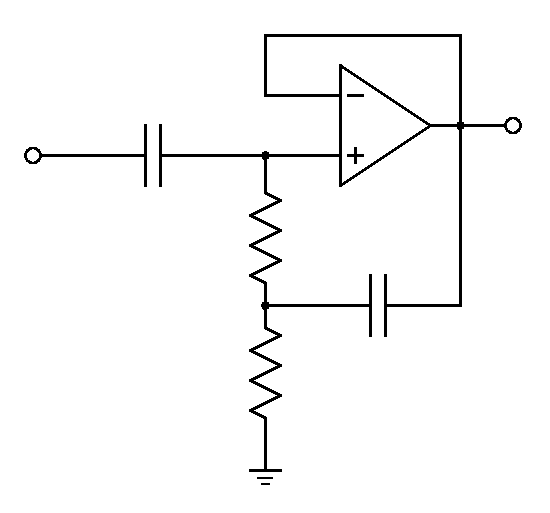
\includegraphics[scale=0.90]{bootstrapOpampBased}
\caption{بدلتا رو مستحکم کار}
\label{شکل_بدلتا_رو_وسطی_دور}
\end{figure}
\عددی{v_S} کا بدلتا جزو \عددی{v_s} مثبت داخلی سرے پر پہنچتا ہے۔یوں \عددی{v_n=v_s} ہو گا جس سے \عددی{v_n=v_k=v_s} اور \عددی{v_o=v_s} ہو گا۔\عددی{C_2} درکار  تعدد پر قصر دور ہو گا اور یوں \عددی{R_1} اور \عددی{R_2} کے جوڑ پر بھی \عددی{v_s} اشارہ پایا جائے گا۔اب دوبارہ داخلی جانب سے سوچیں۔حسابی ایمپلیفائر کا مثبت داخلی سرا  از خود کوئی برقی رو گزرنے نہیں دیتا۔چونکہ مزاحمت \عددی{R_1} کے دونوں سروں پر \عددی{v_s} برقی دباو پایا جاتا ہے لہٰذا اس میں گزرتی برقی رو بھی صفر ہے۔یوں \عددی{v_s} سے کسی قسم کا برقی رو حاصل نہیں کیا جاتا جو کہ منقطع صورت کی نشانی ہے۔یوں بدلتا مستحکم کار درکار تعدد پر لامحدود داخلی مزاحمت پیش کرتے ہوئے حساس اشارے پر بالکل بوجھ نہیں ڈالتا۔

کسی بھی ایمپلیفائر جس کی  \عددی{A_v \approx 1} ہو،  کے  خارجی سرے  سے داخلی جانب یوں کپیسٹر  نسب کر کے اس کا داخلی مزاحمت بڑھایا جا سکتا ہے۔شرط صرف یہ ہے کہ درکار تعدد پر کپیسٹر قصر دور کام کرتے ہوئے مکمل خارجی اشارے کو داخلی جانب مزاحمت \عددی{R_1} تک  پہنچا سکے۔مزاحمت \عددی{R_1} کے ایک سرے کو جس جانب  داخلی اشارہ کھینچتا ہے، خارجی اشارہ بھی اسی جانب مزاحمت کا دوسرا سرا کھینچتا ہے۔

\جزوحصہ{تفرق کار}
ایک اور اہم دور جسے \موٹا{تفرق کار}\فرہنگ{تفرق کار}\فرہنگ{differentiator}\حاشیہب{differentiator}  کہتے ہیں کو شکل \حوالہ{شکل_تفرق_کار} میں دکھایا گیا ہے۔
\begin{figure}
\centering
\includegraphics[scale=0.90]{differentiator}
\caption{تفرق کار}
\label{شکل_تفرق_کار}
\end{figure}
	اس دور کو بالکل پہلی دو ادوار کی طرح حل کرتے ہیں۔جوڑ پر تین برقی رو کے لئے لکھ سکتے ہیں۔
\begin{align} \label{مساوات_تفرق_کار_کے_مساوات_کا_حصول}
i_1 &= C \od{\left (v_n-v_s \right )}{t} \nonumber \\
i_2 &=\frac{v_n-v_o}{R} \nonumber \\
i_3 &=0
\end{align}
جبکہ جوڑ \عددی{v_k} کے لئے لکھ سکتے ہیں۔
\begin{align}
v_k=0
\end{align}
کرچاف کے قانون برائے برقی رو کو جوڑ \عددی{v_n} پر یوں لکھا جا سکتا ہے۔
\begin{align} \label{مساوات_تفرق_کار_داخلی_جوڑ_پر_رو}
i_1+i_2+i_3=0
\end{align}
مساوات \حوالہ{مساوات_تفرق_کار_کے_مساوات_کا_حصول} میں دیے گئے قیمتوں کو مساوات \حوالہ{مساوات_تفرق_کار_داخلی_جوڑ_پر_رو}  میں پر کرتے ہیں
\begin{align*}
C \od{\left(v_n-v_s\right)}{t}+\frac{v_n-v_o}{R}+0&=0
\end{align*}
\عددی{v_n=v_k} لیتے ہوئے  \عددی{v_n=0} کرتے ہوئے
\begin{align*}
 -C \od{v_s}{t}-\frac{v_o}{R}&=0
\end{align*}
حاصل ہوتا ہے جسے یوں لکھ سکتے ہیں۔
\begin{align}
v_o = -RC \od{v_s}{t}
\end{align}
اس مساوات کے تحت یہ دور مہیا کردہ اشارہ \عددی{v_s} کے تفرق کے نسبت سے خارجی اشارہ \عددی{v_o} پیدا کرتا ہے۔اسی سے اس دور کو \موٹا{تفرق کار}\حاشیہب{differentiator}  کہتے ہیں۔


\جزوحصہ{تکمل کار}

تفرقی دور کو دیکھنے کے بعد خیال آتا ہے کہ کیا حسابی ایمپلیفائر کو استعمال کرتے کسی تفاعل کا \موٹا{تکمل}\حاشیہب{integral} حاصل کیا جا سکتا ہے۔جواب ہے جی ہاں۔\موٹا{تکمل کار}\فرہنگ{تکمل کار}\فرہنگ{integrator}\حاشیہب{integrator}  کو شکل \حوالہ{شکل_تکمل_کار}  میں دکھایا گیا ہے۔
\begin{figure}
\centering
\includegraphics[scale=0.90]{integrator}
\caption{تکمل کار}
\label{شکل_تکمل_کار}
\end{figure}
اس دور کے لئے ہم لکھ سکتے ہیں
\begin{gather}
\begin{aligned}
i_1 & = \frac{v_n-v_s}{R} \\
i_2 &= C \od{ (v_n-v_o )}{t} \\
i_3&=0
\end{aligned}
\end{gather}
اور
\begin{align}
v_k =0
\end{align}
کرچاف کا قانون برائے برقی رو استعمال کرتے ہوئے اور \عددی{v_n}  میں \عددی{v_k} کی قیمت (یعنی صفر وولٹ) استعمال کرتے ہوئے حل کرتے ہیں۔
\begin{align*}
i_1+i_2+i_3&=0  \\
\frac{v_n-v_s}{R}+C \od{(v_n-v_o)}{t}+0&=0\\
-\frac{v_s}{R}-C\od{v_o}{t}&=0
\end{align*}
اس کا تکملہ لیتے ہیں
\begin{align*}
\od{v_o}{t}&=-\frac{v_s}{RC}\\
\mathrm{d}v_o&=-\frac{v_s}{RC} \, \mathrm{d}t\\
\int {\mathrm{d}v_o} & =-\int \frac{v_s}{RC} \, \mathrm{d}t
\end{align*}
یعنی
\begin{align} \label{مساوات_حسابی_تکمل_کار}
v_o&=-\frac{1}{RC} \int v_s \, \mathrm{d}t 
\end{align}
اس مساوات میں \عددی{v_o} حاصل کرنے کی خاطر مساوات کے نشان کے دونوں جانب کا تکملہ لیا گیا ہے۔اس طرح تکمل کار کا خارجی اشارہ  \عددی{v_o} اسے مہیا کئے گئے اشارہ\عددی{v_s}کے تکملہ کے براہِ راست متناسب ہوتا ہے۔اسی خاصیت کی وجہ سے اس دور کو \قریب{\موٹا{تکمل کار}}\فرہنگ{تکمل کار}\فرہنگ{integrator}\حاشیہب{integrator}  کہتے ہیں۔

%=================
\ابتدا{مثال}
\عددی{R=\SI{1}{\kilo \ohm}} اور \عددی{C=\SI{6.8}{\micro \farad}} اور \عددی{v_s=V_p \sin \omega t} کی صورت میں
\begin{itemize}
\item
 \موٹا{تکمل کار}  کا خارجی اشارہ حاصل کریں۔
\item
کتنی تعدد پر خارجی اشارے کا حیطہ داخلی اشارے کے حیطے  کے برابر ہو گا۔
\item
خارجی اور داخلی اشارے کا زاویاتی تعلق کیا ہے۔
\end{itemize}
حل:
\begin{itemize}
\item
مساوات \حوالہ{مساوات_حسابی_تکمل_کار} کی مدد سے
\begin{align*}
v_o=-\frac{1}{1000 \times 6.8 \times 10^{-6}} \int V_p \sin \omega t \, \mathrm{d} t=\frac{147 V_p}{\omega} \cos \omega t
\end{align*}
حاصل ہوتا ہے۔
\item
دونوں حیطے برابر اس وقت ہوں گے جب
\begin{align*}
\frac{147 V_p}{\omega}=V_p\\
\omega = 147\\
f=\frac{147}{2 \pi} =\SI{23.396}{\hertz}
\end{align*}
ہو گا۔
\item
داخلی اشارے کو یوں لکھتے ہوئے
\begin{align*}
v_s=V_p \sin \omega t= V_p \cos \left(\omega t-\SI{90}{\degree}\right)
\end{align*}
ہم دیکھتے ہیں کہ داخلی اشارے سے خارجی اشارہ \عددی{\SI{90}{\degree}} \موٹا{آگے}\حاشیہب{leading} ہے۔
\end{itemize}
\انتہا{مثال}
%==============
\ابتدا{مثال}
\عددی{R=\SI{1}{\kilo \ohm}} اور \عددی{C=\SI{10}{\micro \farad}} اور \عددی{v_s=\SI{-0.1}{\volt}} کی صورت میں \عددی{v_o} حاصل کریں۔

حل:
\begin{align*}
v_o=-\frac{1}{1000 \times 10 \times 10^{-6}} \int -0.1 \, \mathrm{d}t =10 t
\end{align*}
حاصل ہوتا ہے۔آپ دیکھ سکتے ہیں کہ خارجی اشارہ وقت کے راست تناسب بڑھتا ہے۔یہ ایک سیکنڈ میں دس وولٹ بڑھ رہا ہے۔اگر داخلی اشارہ مثبت کر دیا جائے تو خارجی اشارہ منفی جانب رواں ہو جائے گا۔
\انتہا{مثال}

شکل \حوالہ{شکل_تکمل_کار_مثال} میں دو مختلف داخلی اشارات پر تکمل کار کا رد عمل دکھایا گیا ہے۔آپ یہاں رک کر تسلی کر لیں کہ خارجی اشارات آپ کے توقع کے عین مطابق ہیں۔
\begin{figure}
\centering
\includegraphics[scale=0.90]{integratorSquareWave}
\caption{تکمل کار کی کارکردگی کے مثال}
\label{شکل_تکمل_کار_مثال}
\end{figure}

%=========================
\جزوحصہ{جمع کار}

حسابی ایمپلیفائر کو دو یا دو سے زیادہ اشارات کا مجموعہ حاصل کرنے کے لئے بھی استعمال کیا جا سکتا ہے۔ایسے ہی \موٹا{جمع کار}\فرہنگ{جمع کار}\فرہنگ{adder}\حاشیہب{adder}  کو شکل \حوالہ{شکل_جمع_کار} میں دکھایا گیا ہے۔
\begin{figure}
\centering
\includegraphics[scale=0.90]{adder}
\caption{جمع کار}
\label{شکل_جمع_کار}
\end{figure}
	اس شکل میں دو اشارات \عددی{v_{s1}} اور \عددی{v_{s2}} مہیا کئے گئے ہیں۔اشارہ \عددی{v_{s1}} مزاحمت \عددی{R_1} کے ذریعہ حسابی ایمپلیفائر کے \عددی{v_n} سرے کے ساتھ جڑا ہے۔اسی طرح اشارہ \عددی{v_{s2}} مزاحمت \عددی{R_2} کے ذریعہ حسابی ایمپلیفائر کے \عددی{v_n} سرے کے ساتھ جڑا ہے۔مزید اشارات کو بھی اسی ترکیب سے جوڑا جا سکتا ہے۔شکل میں دکھائی گئی برقی رو کے لئے یوں لکھ سکتے ہیں۔
\begin{gather}
\begin{aligned}
i_1 &=\frac{v_n-v_{s1}}{R_1} \\
i_2 &=\frac{v_n-v_{s2}}{R_2} \\
i_3&=0 \\
i_o &=\frac{v_n-v_o}{R_0}
\end{aligned}
\end{gather}
اسی طرح جوڑ \عددی{v_k} کے لئے لکھ سکتے ہیں
\begin{align}
v_k =0
\end{align}
جوڑ \عددی{v_n} پر کرچاف کے قانون برائے برقی رو استعمال کرتے ہوئے حل کرتے ہیں۔
\begin{align*}
i_1+i_2+i_3+i_4&=0 \\
\frac{v_n-v_{s1}}{R_1}+\frac{v_n-v_{s2}}{R_2}+0+\frac{v_n-v_o}{R_0}&=0
\end{align*}
\عددی{v_n=v_k} لیتے ہوئے \عددی{v_n=0} پر کرتے ہوئے
\begin{align*}
-\frac{v_{s1}}{R_1}-\frac{v_{s2}}{R_2}-\frac{v_o}{R_0}=0
\end{align*}
حاصل ہوتا ہے جسے
\begin{align}
v_o= -R_0 \left (\frac{v_{s1}}{R_1}+\frac{v_{s2}}{R_2}  \right)
\end{align}
لکھ سکتے ہیں۔\عددیء{R_0}، \عددی{R_1}اور \عددی{R_2} کی قیمتیں برابر ہونے کی صورت میں اس مساوات کو یوں لکھ سکتے ہیں
\begin{align}
v_o = -R \left (\frac{v_{s1}}{R} +\frac{v_{s2}}{R}\right)=- \left (v_{s1}+v_{s2} \right )
\end{align}
اس صورت میں آپ دیکھ سکتے ہیں کہ منفی علامت کے علاوہ، \عددی{v_o}  دونوں اشارات کا مجموعہ ہے۔اسی لئے اس دور کو \موٹا{جمع کار}\فرہنگ{جمع کار}\فرہنگ{adder}\حاشیہب{adder}  کہتے ہیں۔


\جزوحصہ{منفی کار}

حسابی ایمپلیفائر سے دو اشارات منفی کرنے والے دور پر اس حصہ میں غور کرتے ہیں۔ اس دور کو شکل \حوالہ{شکل_منفی_کار} میں دکھایا گیا ہے۔
\begin{figure}
\centering
\includegraphics[scale=0.90]{subtractor}
\caption{منفی کار}
\label{شکل_منفی_کار}
\end{figure}
شکل کو دیکھتے ہم لکھ سکتے ہیں۔
\begin{gather}
\begin{aligned}
i_1 &= \frac{v_n-v_{s1}}{R_1}\\
i_2&=\frac{v_n-v_o}{R_2}\\
i_3&=\frac{v_k-v_{s2}}{R_3}\\
i_4&=\frac{v_k}{R_4}\\
i_5&=0\\
i_6&=0
\end{aligned}
\end{gather}
انہیں کرچاف کے قانون برائے برقی رو میں  استعمال کرتے ہوئے، جوڑ \عددی{v_n}  کے لئے یوں لکھ سکتے ہیں۔
\begin{gather} \label{مساوات_منفی_کار_منفی_سرے_پر_دباو}
\begin{aligned}
 i_1+i_2+i_5=0\\
\frac{v_n-v_{s1}}{R_1}+\frac{v_n-v_o}{R_2}+0=0\\
v_n \left(\frac{1}{R_1}+\frac{1}{R_2} \right)=\frac{v_{s1}}{R_1}+\frac{v_o}{R_2}\\
v_n=\frac{\frac{v_{s1}}{R_1}+\frac{v_o}{R_2}}{\frac{1}{R_1}+\frac{1}{R_2}}
\end{aligned}
\end{gather}
اسی طرح جوڑ \عددی{v_k}  پر کرچاف کا قانون برائے برقی رو لاگو کرتے ہوئے اسے یوں حل کر سکتے ہیں۔
\begin{gather} \label{مساوات_منفی_کار_مثبت_سرے_پر_دباو}
\begin{aligned}
i_3+i_4+i_6=0\\
\frac{v_k-v_{s2}}{R_3}+\frac{v_k}{R_4}+0=0\\
v_k \left(\frac{1}{R_3}+\frac{1}{R_4} \right)=\frac{v_{s2}}{R_3}\\
v_k=\frac{\frac{v_{s2}}{R_3}}{\frac{1}{R_3}+\frac{1}{R_4} }
\end{aligned}
\end{gather}
مساوات \حوالہ{مساوات_حسابی_بنیادی_پہلو} کی پہلی شق کے تحت \عددی{v_k}  اور \عددی{v_n} برابر ہوتے ہیں۔یوں مساوات \حوالہ{مساوات_منفی_کار_منفی_سرے_پر_دباو}  اور \حوالہ{مساوات_منفی_کار_مثبت_سرے_پر_دباو}  کو برابر ڈالتے ہوئے
\begin{align*}
v_n=v_k\\
\frac{\frac{v_{s1}}{R_1}+\frac{v_o}{R_2}}{\frac{1}{R_1}+\frac{1}{R_2}}=\frac{\frac{v_{s2}}{R_3}}{\frac{1}{R_3}+\frac{1}{R_4} }
\end{align*}
یعنی
\begin{gather}
\begin{aligned} \label{مساوات_حسابی_منفی_کار}
v_o&=\frac{R_4}{R_1} \left(\frac{R_1+R_2}{R_3+R_4} \right) v_{s2}-\frac{R_2}{R_1}v_{s1}\\
&=\left(\frac{1+\frac{R_2}{R_1}}{1+\frac{R_3}{R_4}} \right) v_{s2}-\frac{R_2}{R_1}v_{s1}
\end{aligned}
\end{gather}
حاصل ہوتا ہے۔یہ دور کی عمومی مساوات ہے۔اگر دور میں \عددی{R_1=R_3=R_a} جبکہ \عددی{R_2=R_4=R_b} ہوں تب اس مساوات سے
\begin{align}
v_o=\frac{R_b}{R_a}\left(v_{s2}-v_{s1}\right)
\end{align}
حاصل ہوتا ہے۔اگر \عددی{R_a}  اور\عددی{R_b} کی قیمتیں برابر ہوں تو اس صورت میں دور دونوں اشارات کو منفی کرے گا۔اسی لئے اس دور کو \موٹا{منفی کار}\فرہنگ{منفی کار}\فرہنگ{subtractor}\حاشیہب{subtractor} کہتے ہیں۔اگر\عددی{R_a} اور \عددی{R_b}برابر نہ ہوں تو دور دونوں اشارات میں فرق کو بڑھانے یا گھٹانے کی صلاحیت بھی رکھتا ہے

\ابتدا{مثال}
منفی کار کا مشترکہ داخلی مزاحمت تمام مزاحمت برابر ہونے کی صورت میں حاصل کریں۔تمام مزاحمت مختلف ہونے کی صورت میں جواب کیا ہو گا۔

\begin{figure}
\centering
\includegraphics[scale=0.90]{subtractorExample}
\caption{منفی کار کا مشترکہ داخلی مزاحمت}
\label{شکل_منفی_کار_مشترکہ_داخلی_مزاحمت}
\end{figure}
حل:
مشترکہ داخلی مزاحمت حاصل کرنے کی خاطر دونوں داخلی سروں  کو آپس میں جوڑتے ہوئے ان پر مشترکہ اشارہ \عددی{v_s} لاگو کیا جاتا ہے۔اشارے سے \عددی{i_a} اور \عددی{i_b} برقی رو منفی کار میں داخل ہوں گے۔مشترکہ مزاحمت داخلی برقی دباو اور داخلی برقی رو کے مجموعہ کی شرح کو کہتے ہیں یعنی
\begin{align*}
R_{\textup{مشترک}}=\frac{v_s}{i_a+i_b}
\end{align*} 
آئیں داخلی مزاحمت کو پہلے حساب و کتاب سے حاصل کریں۔تمام مزاحمت \عددی{R} کے برابر ہونے کی صورت میں
\begin{align*}
v_0=0\\
v_k=\frac{v_s}{2}\\
v_n=\frac{v_s}{2}
\end{align*}
حاصل ہوتے ہیں۔لہٰذا
\begin{align*}
i_a=\frac{v_s-v_n}{R}=\frac{v_s}{2R}\\
i_b=\frac{v_s-v_k}{R}=\frac{v_s}{2R}\\
i_a+i_b=\frac{v_s}{R}
\end{align*}
اور یوں
\begin{align*}
R_{\textup{داخلی}}=R
\end{align*}
حاصل ہوتا ہے۔

اس جواب کو یوں بھی حاصل کیا جا سکتا ہے۔حسابی ایمپلیفائر کے دونوں داخلی سروں  پر داخلی برقی رو صفر ہوتی ہے۔\عددی{v_k} پر داخلی برقی رو صفر  ہونے کی وجہ سے اسے کھلے سرے تصور کیا جا سکتا ہے۔اس طرح  \عددی{R_3} اور \عددی{R_4} کو \عددی{v_s} اور برقی زمین کے مابین سلسلہ وار جڑا تصور کیا جا سکتا ہے۔تمام مزاحمت برابر ہونے کی وجہ سے \عددی{v_o=\SI{0}{\volt}} ہے لہٰذا اسے برقی زمین تصور کیا جا سکتا ہے۔\عددی{v_n} پر برقی رو صفر ہونے کی وجہ سے اس داخلی سرے  کو بھی کھلے سرے تصور کیا جا سکتا ہے۔یوں \عددی{R_1} اور \عددی{R_2} کو بھی \عددی{v_s} اور برقی زمین کے مابین سلسلہ وار جڑا تصور کیا جا سکتا ہے۔اس طرح سلسلہ وار جڑے \عددی{R_1} اور \عددی{R_2} کو سلسلہ وار جڑے \عددی{R_3} اور \عددی{R_4} کے متوازی تصور کیا جا سکتا ہے لہٰذا
\begin{align*}
\frac{1}{R_{\textrm{داخلی}}}&=\frac{1}{R_1+R_2}+\frac{1}{R_3+R_4}=\frac{1}{2R}+\frac{1}{2R}=\frac{1}{R}\\
R_{\textrm{داخلی}}&=R
\end{align*}
حاصل ہوتا ہے۔

تمام مزاحمت مختلف ہونے کی صورت میں مساوات \حوالہ{مساوات_حسابی_منفی_کار} سے خارجی اشارہ  یوں حاصل ہوتا ہے۔
\begin{align*}
v_o=\left[\left(\frac{R_1+R_2}{R_3+R_4} \right)\frac{R_4}{R_1}-\frac{R_2}{R_1} \right]v_s
\end{align*}
حسابی ایمپلیفائر کے دونوں داخلی سروں  پر داخلی برقی رو صفر ہونے کی وجہ سے \عددی{R_1} اور \عددی{R_2} میں یکساں برقی رو \عددی{i_a} پایا جائے گا۔اسی طرح \عددی{R_3} اور \عددی{R_4} میں \عددی{i_b} پایا جائے گا جہاں
\begin{align*}
i_a&=\frac{v_s-v_0}{R_1+R_2}\\
&=v_s\left[\frac{1}{R_1+R_2}-\frac{R_4}{R_1 \left(R_3+R_4 \right)}+\frac{R_2}{R_1 \left(R_1+R_2 \right)} \right]\\
&=\frac{R_3 v_s}{R_1\left(R_3+R_4 \right)}\\
i_b&=\frac{v_s}{R_3+R_4}
\end{align*}
کے برابر ہیں۔یوں
\begin{align*}
R_{\textrm{داخلی}}=\frac{v_s}{i_a+i_b}=\frac{R_1 \left(R_3+R_4 \right)}{R_1+R_3}
\end{align*}
حاصل ہوتا ہے۔

اسی جواب کو قدر آسان طریقے سے یوں حاصل کیا جا سکتا ہے۔حسابی ایمپلیفائر کے مثبت داخلی سرے  کو کھلے سرے تصور کیا جا سکتا ہے۔اس طرح \عددی{R_3} اور \عددی{R_4} کو \عددی{v_s} اور برقی زمین کے مابین دو سلسلہ وار جڑے مزاحمت تصور کیا جا سکتا ہے۔ان دو مزاحمتوں میں برقی دباو کے تقسیم سے
\begin{align*}
v_k=\frac{R_4 v_s}{R_3+R_4}
\end{align*}
حاصل ہوتا ہے۔اسی طرح ان میں برقی رو
\begin{align*}
i_b=\frac{v_s}{R_3+R_4}
\end{align*}
حاصل ہوتا ہے۔\عددی{v_k=v_n} ہونے کی بدولت \عددی{v_n} بھی یہی ہو گا۔لہٰذا \عددی{R_1} میں برقی رو
\begin{align*}
i_a&=\frac{v_s-v_n}{R_1}=\frac{v_s-\frac{R_4 v_s}{R_3+R_4}}{R_1}
\end{align*}
ہو گا۔ان دو برقی رو سے داخلی مزاحمت حاصل ہوتا ہے۔\عددی{v_n} کی قیمت \عددی{v_k} تعین کرتا ہے۔چونکہ \عددی{v_k} کا دارومدار مزاحمت \عددی{R_3} اور \عددی{R_4} پر ہے  جبکہ \عددی{i_a} کا دارومدار \عددی{v_n} اور \عددی{R_1} پر ہے لہٰذا \عددی{i_a} اور \عددی{i_b} دونوں پر \عددی{R_2} کا کوئی اثر نہیں۔اسی لئے داخلی مزاحمت میں \عددی{R_2} کا کوئی کردار نہیں۔
\انتہا{مثال}
%==============
\ابتدا{مثال} \شناخت{مثال_حسابی_منفی_مزاحمت_غلطی}
\موٹا{منفی کار} کے تمام مزاحمت برابر ہونے کی صورت میں دونوں داخلی سروں  پر مشترکہ داخلی اشارہ \عددی{v_s} مہیا کرنے سے \عددی{v_0=\SI{0}{\volt}} حاصل ہوتا ہے۔اس صورت میں منفی کار کی مشترکہ افزائش صفر حاصل ہوتی ہے۔\عددی{\SI{6.8}{\kilo \ohm} \pm \SI{5}{\percent}} کے مزاحمت استعمال کرتے ہوئے ایمپلیفائر کی خراب سے خراب تر مشترکہ افزائش کیا ممکن ہے۔مشترکہ افزائش جتنی زیادہ ہو اتنا ہی اسے خراب سمجھا جاتا ہے۔ 

حل:
مساوات \حوالہ{مساوات_حسابی_منفی_کار} کے مطابق مشترکہ داخلی اشارے کی صورت (\عددی{v_{s2}=v_{s1}=v_s}) میں  مشترکہ افزائش
\begin{align*}
\frac{v_o}{v_s}&=\left(\frac{R_1+R_2}{R_3+R_4} \right) \frac{R_4}{R_1}-\frac{R_2}{R_1}\\
&=\frac{R_1 R_4-R_2R_3}{R_1 \left(R_3+R_4 \right)}\\
&=\frac{1-\frac{R_2R_3}{R_1 R_4}}{1+\frac{R_3}{R_4}}
\end{align*}
حاصل ہوتی ہے۔اس مساوات میں \عددی{v_o} کی زیادہ سے زیادہ قیمت اس صورت حاصل ہو گی جب \عددی{\tfrac{R_3}{R_4}} اور  \عددی{\tfrac{R_2 R_3}{R_1R_4}}  کے قیمت کم سے کم ہوں۔\عددی{\tfrac{R_3}{R_4}} کی قیمت کم سے کم تب ہو گی جب \عددی{R_3} پانچ فی صد کم اور \عددی{R_4} پانچ فی صد زیادہ ہو یعنی جب \عددی{R_3=\SI{6.46}{\kilo \ohm}} اور \عددی{R_4=\SI{7.14}{\kilo \ohm}} ہوں۔اسی طرح \عددی{\tfrac{R_2 R_3}{R_1R_4}} کی قیمت کم سے کم تب ہو گی جب \عددی{R_2=\SI{6.46}{\kilo \ohm}} اور \عددی{R_1=\SI{7.14}{\kilo \ohm}} ہوں گے۔ان قیمتوں کے استعمال سے خراب سے خراب تر مشترکہ افزائش
\begin{align*}
\frac{v_o}{v_s}=\frac{1-\frac{6.46 \times 6.46}{7.14 \times 7.14}}{1+\frac{6.46}{7.14}}=\SI{0.095238}{\volt \per \volt}
\end{align*}
حاصل ہوتی ہے۔

\انتہا{مثال}
%============
\ابتدا{مثال}
مثال \حوالہ{مثال_حسابی_منفی_مزاحمت_غلطی} میں تمام مزاحمت مختلف ہونے کی صورت میں مزاحمت کے قیمت میں غلطی کی وجہ سے خراب تر مشترکہ افزائش کی عمومی جواب حاصل کریں۔

حل:
گزشتہ مثال میں 
\begin{align*}
\frac{v_o}{v_s}=\frac{1-\frac{R_2R_3}{R_1 R_4}}{1+\frac{R_3}{R_4}}
\end{align*}
حاصل کی گئی۔جیسا وہاں بتلایا گیا \عددی{R_2} اور \عددی{R_3} کے قیمت کم سے کم یعنی \عددی{\left(1-\epsilon \right) R_2} اور \عددی{\left(1-\epsilon \right) R_3} جبکہ \عددی{R_1} اور \عددی{R_4} کے قیمت زیادہ سے زیادہ یعنی \عددی{\left(1+\epsilon \right) R_1} اور
 \عددی{\left(1+\epsilon \right) R_4} ہونے ہوں گے۔اس طرح
\begin{align*}
\frac{v_o}{v_s}=\frac{1-\left(\frac{1-\epsilon}{1+\epsilon}\right)^2\frac{R_2R_3}{R_1 R_4}}{1+\left(\frac{1-\epsilon}{1+\epsilon}\right)\frac{R_3}{R_4}}
\end{align*}
حاصل ہوتا ہے۔تمام مزاحمت ایک ہی قیمت کے ہونے کی صورت میں
\begin{align*}
\frac{v_o}{v_s}=\frac{2 \epsilon}{1+\epsilon}
\end{align*}
حاصل ہوتا ہے۔

\انتہا{مثال}

آپ نے حسابی ایمپلیفائر پر مبنی کئی ادوار دیکھے۔یہ ادوار جمع، منفی، تفرق اور تکملہ جیسے حسابی اعمال سرانجام دیتے ہیں یا پھر اشارات کی افزائش کرتے ہیں۔انہیں خوبیوں کی بدولت ہم اسے \موٹا{حسابی ایمپلیفائر}  پکارتے ہیں۔\فرہنگ{حسابی ایمپلیفائر}\فرہنگ{OPAMP}\حاشیہب{OPAMP}

\جزوحصہ{جمع و منفی کار}
شکل \حوالہ{شکل_جمع_و_منفی_کار} میں متعدد داخلی سروں  والا \موٹا{جمع و منفی کار} دکھایا گیا ہے۔مثبت داخلی سروں  پر \عددی{v_{j1}} تا \عددی{v_{js}} جبکہ منفی داخلی سروں  پر \عددی{v_{m1}} تا \عددی{v_{mn}} اشارات مہیا کئے گئے ہیں۔آئیں اس دور کو حل کریں۔
جوڑ \عددی{v_n} پر کرچاف کے قانون برائے برقی رو سے ہم لکھ سکتے ہیں
\begin{align*}
\frac{v_n-v_{m1}}{R_{m1}}+\frac{v_n-v_{m2}}{R_{m2}} \cdots +\frac{v_n-v_{mn}}{R_{mn}}+\frac{v_n-v_o}{R_0}=0\\
v_n \left(\frac{1}{R_{m1}}+\frac{1}{R_{m2}}\cdots +\frac{1}{R_{mn}}+\frac{1}{R_0} \right)=\frac{v_{m1}}{R_{m1}}+\frac{v_{m2}}{R_{m2}}\cdots +\frac{v_{mn}}{R_{mn}}+\frac{v_o}{R_0}
\end{align*}
جس میں
\begin{align*}
\frac{1}{R_{m1}}+\frac{1}{R_{m2}}\cdots +\frac{1}{R_{mn}}=\frac{1}{R_m}
\end{align*}
لکھتے ہوئے
\begin{align*}
v_n \left(\frac{1}{R_m}+\frac{1}{R_0} \right)=\frac{v_{m1}}{R_{m1}}+\frac{v_{m2}}{R_{m2}}\cdots +\frac{v_{mn}}{R_{mn}}+\frac{v_o}{R_0}\\
v_n=\left(\frac{R_mR_0}{R_m+R_0} \right)\left(\frac{v_{m1}}{R_{m1}}+\frac{v_{m2}}{R_{m2}}\cdots +\frac{v_{mn}}{R_{mn}}+\frac{v_o}{R_0} \right)
\end{align*}
حاصل ہوتا ہے۔اسی طرح جوڑ \عددی{v_k} کے لئے حل کرتے ہیں۔
\begin{align*}
\frac{v_k-v_{j1}}{R_{j1}}+\frac{v_k-v_{j2}}{R_{j2}}\cdots +\frac{v_k-v_{js}}{R_{js}}=0\\
v_k \left(\frac{1}{R_{j1}}+ \frac{1}{R_{j2}}\cdots + \frac{1}{R_{js}}\right)=\frac{v_{j1}}{R_{j1}}+\frac{v_{j2}}{R_{j2}}\cdots+\frac{v_{js}}{R_{js}}
\end{align*}
جس میں
\begin{align*}
\frac{1}{R_{j1}}+ \frac{1}{R_{j2}}\cdots + \frac{1}{R_{js}}=\frac{1}{R_{j}}
\end{align*}
استعمال کرتے ہوئے 
\begin{align*}
v_k=\frac{R_j }{R_{j1}}v_{j1}+\frac{R_j }{R_{j2}}v_{j2}\cdots+\frac{R_j }{R_{js}}v_{js}
\end{align*}
حاصل ہوتا ہے۔\عددی{v_n=v_k} لکھتے ہوئے \عددی{v_o} کے لئے حل کرتے ہوئے حاصل ہوتا ہے۔
\begin{align} \label{مساوات_حسابی_جمع_و_منفی_کار}
v_0&=\left( 1+\frac{R_0}{R_m}\right)\left(\frac{R_j }{R_{j1}}v_{j1}+\frac{R_j }{R_{j2}}v_{j2}\cdots \right. \\
& \qquad  \qquad \left. \cdots +\frac{R_j }{R_{js}}v_{js} \right)-\left(\frac{R_0}{R_{m1}}v_{m1}+\frac{R_0}{R_{m2}}v_{m2}\cdots +\frac{R_0}{R_{mn}}v_{mn}\right)
\end{align}

%
\begin{figure}
\centering
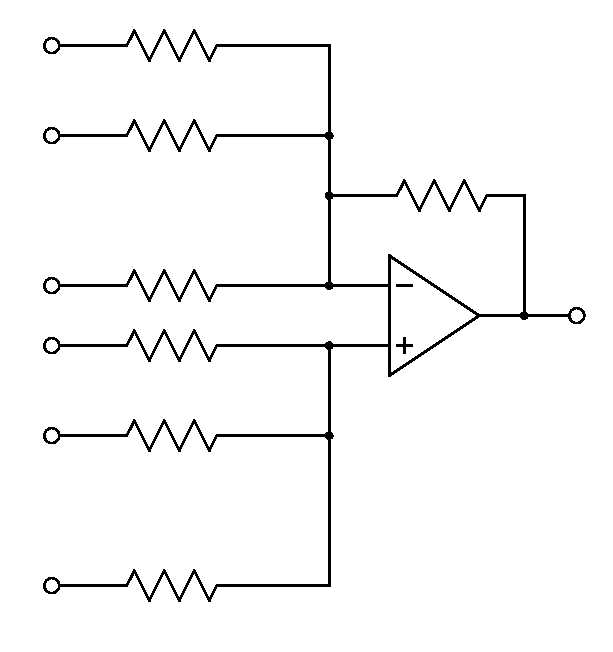
\includegraphics[scale=0.90]{adderSubtractorExample}
\caption{جمع و منفی کار}
\label{شکل_جمع_و_منفی_کار}
\end{figure}

\جزوحصہ{آلاتی ایمپلیفائر}

حسابی ایمپلیفائر پر تبصرہ کرتے ہوئے \موٹا{آلاتی ایمپلیفائر}\فرہنگ{آلاتی ایمپلیفائر}\فرہنگ{amplifier!instrumentation}\حاشیہب{instrumentation amplifier} کا ذکر کرنا لازم ہے۔\موٹا{آلاتی ایمپلیفائر} باریک اور حساس اشارات کے حصول کے لئے استعمال کیا جاتا ہے۔موجودہ دور میں ہر قسم کے طبعی متغیرات کو برقی اشارات میں تبدیل کر کے ان پر کمپیوٹر کی مدد سے غور کیا جاتا ہے۔آپ \موٹا{برقی قلب نگار}\فرہنگ{برقی!قلب نگار}\فرہنگ{ecg}\حاشیہب{ecg} سے بخوبی واقف ہوں گے جو دل کے کارکردگی کے اشارات کھینچتا ہے۔\موٹا{برقی قلب نگار} کو \موٹا{آلاتی ایمپلیفائر} کے مدد سے ہی بنایا جاتا ہے۔\حاشیہد{آج مورخہ 21 مارچ 2014 کو میری بیٹی عفت بریخنہ  نے انجنیئرنگ کے آخری سال کے پڑھائی کے دوران آلاتی ایمپلیفائر سے برقی قلب نگار بناتے ہوئے دل کی دھڑکن کے اشارات حاصل کئے۔}

ان حساس اشارات کے حصول کے لئے زیادہ سے زیادہ \موٹا{داخلی برقی رکاوٹ}\فرہنگ{داخلی برقی رکاوٹ}\حاشیہب{input impedance}  والے ادوار استعمال کئے جاتے ہیں۔ایسے جگہوں پر عموماً \موٹا{آلاتی ایمپلیفائر} استعمال کیا جاتا ہے جس کا داخلی برقی رکاوٹ لامحدود تصور کیا جا سکتا ہے۔\موٹا{آلاتی ایمپلیفائر}  کو شکل \حوالہ{شکل_آلاتی_ایمپلیفائر} میں دکھایا گیا ہے۔
\begin{figure} \label{شکل_حسابی_آلاتی_ایمپلیفائر}
\centering
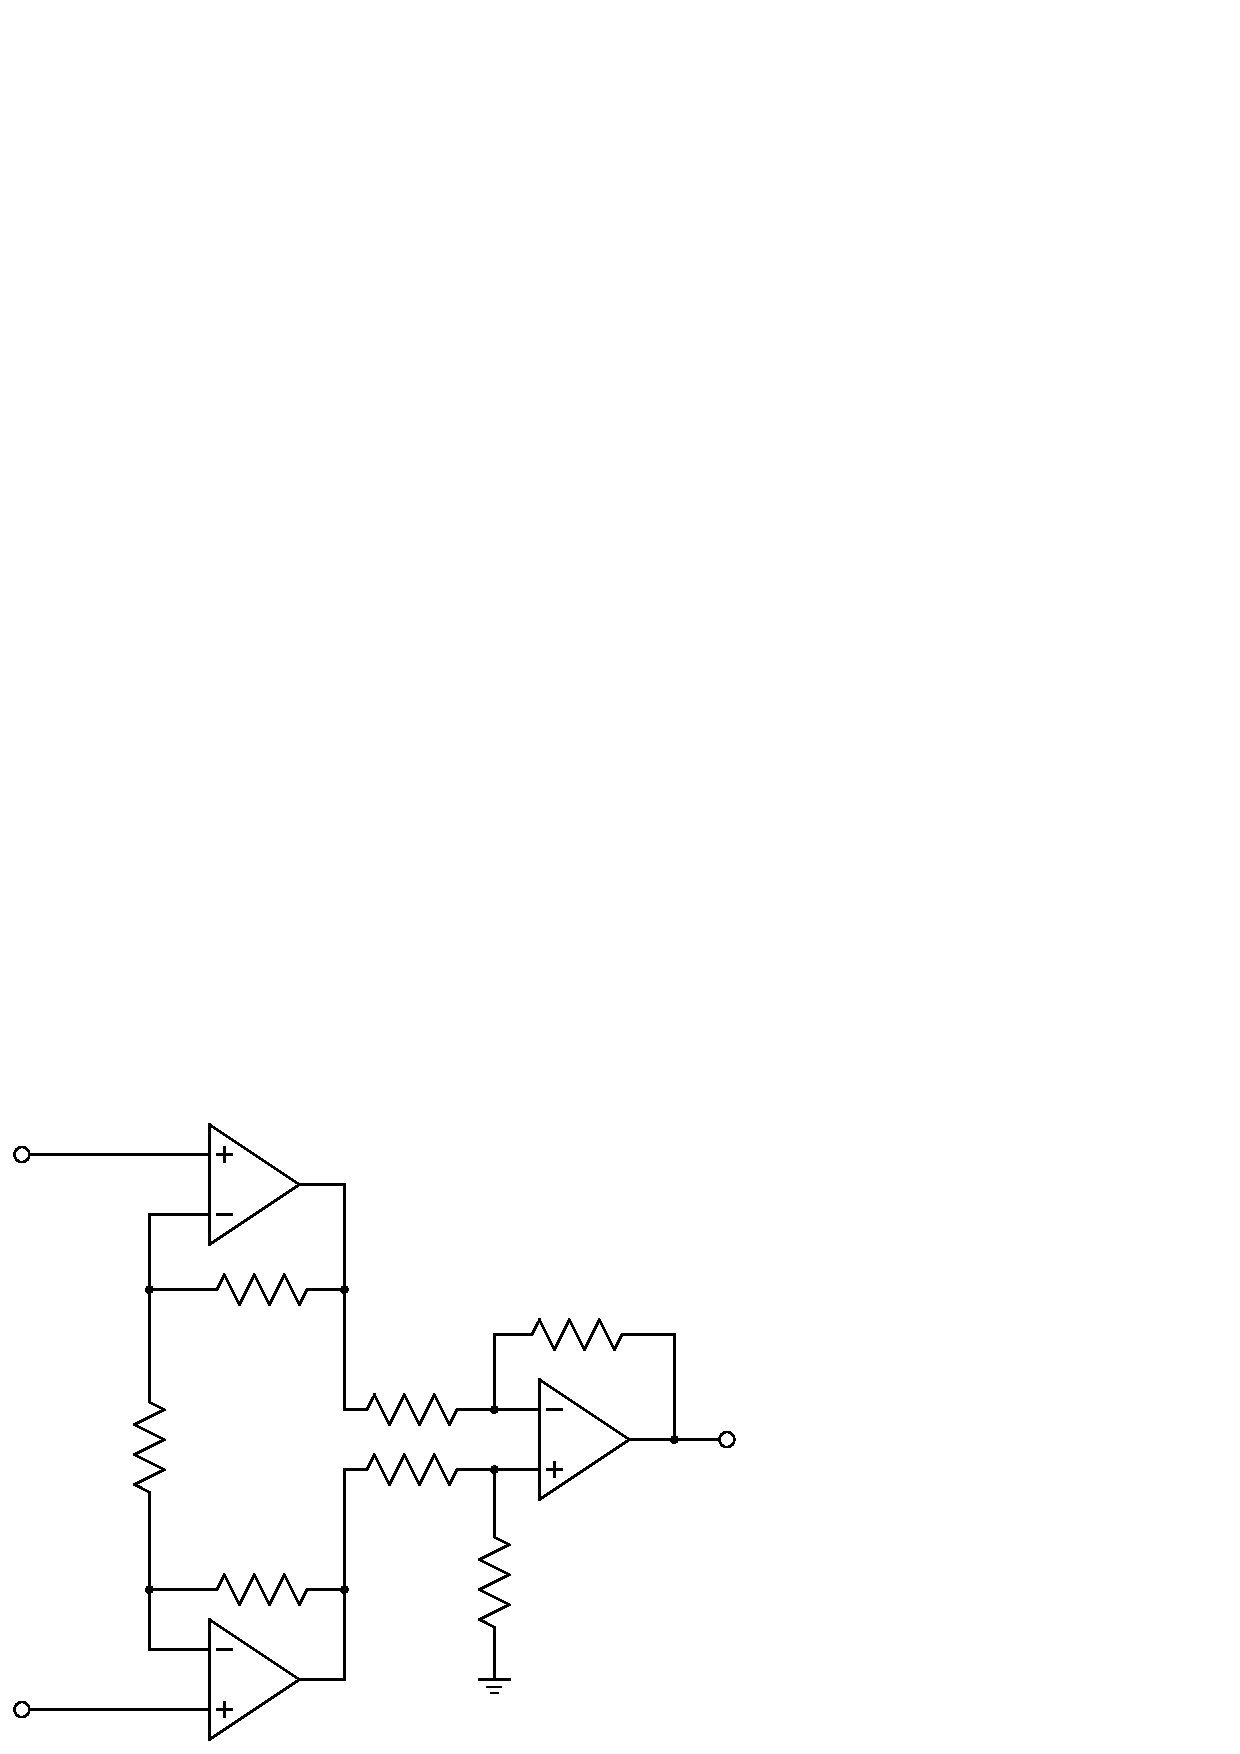
\includegraphics[scale=0.90]{instrumentationAmplifier}
\caption{آلاتی ایمپلیفائر}
\label{شکل_آلاتی_ایمپلیفائر}
\end{figure}
اس دور میں  \عددی{v_1} اور \عددی{v_2} داخلی اشارات ہیں۔کسی بھی حسابی ایمپلیفائر کے داخلی سروں پر برقی دباو برابر رہتا ہے۔یوں \عددی{v_{n1}=v_{k1}=v_1} اور  \عددی{v_{n2}=v_{k2}=v_2} ہو گا۔اس طرح مزاحمت \عددی{R_1} کے نیچے جانب سرے پر برقی دباو کی قیمت \عددی{v_2} اور اس کے اوپر جانب سرے پر برقی دباو کی قیمت \عددی{v_1} ہو گی۔یوں \عددی{R_1} کے سروں کے مابین برقی دباو کی قیمت \عددی{(v_2-v_1)} ہو گی اور اس میں برقی رو
\begin{align}
i_{R_1}=\frac{v_2-v_1}{R_1}
\end{align}
ہو گی۔

جوڑ \عددی{v_{n1}}  پر کرچاف کے قانون برائے برقی رو لاگو کرنے سے ثابت ہوتا ہے کہ اس جوڑ پر نسب \عددی{R_2} میں \عددی{i_{R_1}} کے برابر برقی رو گزرے گی جسے شکل میں تیر کے نشان سے دکھایا گیا ہے۔اسی طرح جوڑ \عددی{v_{n2}} پر کرچاف کے قانون سے ثابت ہوتا ہے کہ اس جوڑ پر نسب \عددی{R_2} میں بھی \عددی{i_{R_1}} گزرے گی جسے تیر کے نشان سے دکھایا گیا ہے۔اس طرح \عددی{i_{R_1}} تین سلسلہ وار جڑی مزاحمت \عددی{R_2} ، \عددی{R_1} اور  \عددی{R_2} سے گزرتی ہے۔ان سلسلہ وار جڑے مزاحمتوں کے آخری سروں کے مابین برقی دباو کو یوں لکھ سکتے ہیں۔
\begin{gather}
\begin{aligned}
v_{o2}-v_{o1}&= i_{R_1} \times \left (R_2+R_1+R_2 \right )\\
&=\frac{\left (v_2-v_1 \right )}{R_1} \left (R_1+2 R_2 \right )\\
&=\left (1+\frac{2 R_2}{R_1}\right ) \left (v_2-v_1 \right )
\end{aligned}
\end{gather}
اس برقی دباو کو خارجی جانب منفی کار کو مہیا کیا جاتا ہے اور یوں 
\begin{align}
v_o = \frac{R_4}{R_3}\left (v_{o2}-v_{o1} \right ) =\frac{R_4}{R_3} \left (1+\frac{2 R_2}{R_1} \right ) \left (v_2-v_1 \right )
\end{align}
جو کہ آلاتی ایمپلیفائر کی درکار مساوات ہے۔

\ابتدا{مثال}
ایک آلاتی ایمپلیفائر میں
\begin{align*}
R_1=\SI{500}{\ohm} \hspace{5mm} R_2=\SI{50}{\kilo \ohm}\\
R_3=\SI{10}{\kilo \ohm} \hspace{5mm} R_4=\SI{10}{\kilo \ohm}\\
v_2=4+0.003 \sin \omega t\\
v_1=4-0.003 \sin \omega  t
\end{align*}
ہیں۔آلاتی ایمپلیفائر کے ہر جوڑ پر برقی دباو حاصل کریں۔\موٹا{مشترک اشارہ رد کرنے کی صلاحیت} \عددی{CMRR} حاصل کریں۔

حل:

دونوں داخلی سروں  پر یکساں برقی دباو کو مشترکہ برقی دباو کہتے ہیں جبکہ دونوں داخلی سروں  کے مابین برقی دباو کو تفرق برقی دباو کہتے ہیں۔یوں
\begin{align*}
v_{\textrm{مشترک}}&=\SI{4}{\volt}\\
v_{\textup{تفرق}}&=0.06 \sin \omega t
\end{align*}
ہیں۔یوں انہیں
\begin{align*}
v_2=v_{\textrm{مشترک}}+ \frac{v_{\textrm{تفرق}}}{2}\\
v_1=v_{\textrm{مشترک}}-\frac{v_{\textrm{تفرق}}}{2}
\end{align*}
لکھا جا سکتا ہے۔

جوڑ \عددی{v_{n1}} پر \عددی{v_1} جبکہ جوڑ \عددی{v_{n2}} پر \عددی{v_2} پایا جائے گا۔یوں \عددی{R_1} میں برقی رو کی قیمت
\begin{align*}
I_{R1}=\frac{\left(4+0.003 \sin \omega t \right)-\left(4-0.003 \sin \omega t \right)}{500}=12 \times 10^{-6} \sin \omega t
\end{align*}
 ہو گی۔یوں مزاحمت \عددی{R_2} کے دو سروں کے مابین برقی دباو  کی قیمت
\begin{align*}
12 \times 10^{-6} \sin \omega t \times 50 \times 10^3=0.6 \sin \omega t
\end{align*}
ہو گی۔نچلے \عددی{R_2} میں برقی رو کی سمت مزاحمت کے دائیں سرے سے بائیں سرے کی جانب ہے۔یوں اس کا دایاں سرا مثبت جبکہ بایاں سرا منفی ہو گا۔چونکہ ان سروں پر برقی دباو کو \عددی{v_{o2}} اور \عددی{v_{n2}} کہا گیا ہے لہٰذا
\begin{align*}
v_{o2}-v_{n2}&=0.6 \sin \omega t\\
v_{o2}&=4+0.003 \sin \omega t +0.6 \sin \omega t\\
&=4+0.603 \sin \omega t
\end{align*}
ہو گا۔اسی طرح اوپر والے \عددی{R_2} میں برقی رو کی سمت \عددی{v_{n1}} سے \عددی{v_{o1}} کے جانب ہے لہٰذا
\begin{align*}
v_{n1}-v_{o1}&=0.6 \sin \omega t\\
v_{o1}&=4-0.003 \sin \omega t -0.6 \sin \omega t\\
&=4-0.603 \sin \omega t
\end{align*}
حاصل ہو گا۔یہاں رک کر نتائج پر غور کریں۔مشترکہ اشارہ جوں کا توں ہے جبکہ تفرق اشارہ دونوں خارجی سروں  پر  بڑھ گیا ہے۔\عددی{v_{o2}} اور \عددی{v_{o1}} کو منفی کار کے حوالے کیا جاتا ہے۔منفی کار  کے مثبت داخلی سرا \عددی{v_k} پر کرچاف کے قانون برائے برقی رو لکھتے ہوئے
\begin{align*}
&\frac{v_k-v_{o2}}{R_3}+\frac{v_k}{R_4}=0\\
v_k&=\left(\frac{R_4}{R_3+R_4} \right) v_{o2}\\
&=2+0.2015 \sin \omega t
\end{align*}
حاصل ہوتا ہے۔\عددی{v_n} اور \عددی{v_k} برابر ہونے کی وجہ سے \عددی{v_n} بھی یہی ہو گا۔مندرجہ بالا جواب \عددی{R_3} اور \عددی{R_4} کو سلسلہ وار \عددی{v_{o2}} اور برقی زمین کے مابین جڑا تصور کرتے ہوئے برقی دباو کے تقسیم کی مساوات سے بھی حاصل ہوتا ہے۔منفی کار کا خارجی اشارہ
\begin{align*}
v_o&=\frac{R_4}{R_3}{\left(v_{o2}-v_{o1} \right)}\\
&=\frac{10000}{10000} \left[\left(4+0.603 \sin \omega t\right)-\left(4-0.603 \sin \omega t \right) \right]\\
&=1.206 \sin \omega t
\end{align*}
حاصل ہوتا ہے۔

چونکہ خارجی اشارے میں مشترکہ اشارے کا نام و نشان تک نہیں لہٰذا مشترکہ افزائش صفر کے برابر ہے یعنی \عددی{A_m=0} جبکہ تفرقی افزائش کو مندرجہ بالا مساوات سے یوں حاصل کیا جا سکتا ہے۔
\begin{align*}
A_d=\frac{v_o}{v_d}=\frac{1.206 \sin \omega t}{0.06 \sin \omega t}=201
\end{align*}
اس طرح مشترکہ اشارہ رد کرنے کی صلاحیت
\begin{align*}
CMRR=\frac{A_d}{A_m}=\infty
\end{align*}
حاصل ہوتا ہے۔
\انتہا{مثال}

اس مثال میں آلاتی ایمپلیفائر نے مشترکہ اشارے کو مکمل رد کرتے ہوئے تفرق اشارے کو \عددی{201} گنا بڑھایا۔یہاں اس بات پر توجہ دیتے ہوئے ذھن نشین کریں کہ مزاحمتوں کے قیمتیں جس طرح بھی رکھی جائیں \عددی{v_{o2}} اور \عددی{v_{o1}} میں کسی صورت بھی مشترکہ اشارہ بڑھتا نہیں۔یہ جوں کا توں ان دو خارجی سروں  پر پایا جاتا ہے۔آلاتی ایمپلیفائر کا دوسرا حصہ یعنی \موٹا{منفی کار} \عددی{v_{o2}} سے \عددی{v_{o1}} منفی کرتے ہوئے مشترکہ اشارے کو مکمل طور رد کر دیتا ہے۔تفرق اشارے کو آلاتی ایمپلیفائر کے دونوں حصے بڑھانے کی صلاحیت رکھتے ہیں۔اگلے مثال میں ان حقائق پر مزید غور کیا جائے گا۔

آلاتی ایمپلیفائر میں دونوں مزاحمت جنہیں \عددی{R_2} لکھا گیا ہے کے قیمتیں برابر رکھی جاتی ہیں۔البتہ مزاحمت کے قیمتوں میں غلطی کی بنا پر ان کی قیمت
 \عددی{\left(1 - \epsilon \right) R_2} تا  \عددی{\left(1 + \epsilon \right) R_2} ممکن ہوتی ہیں۔مزاحمت کے قیمت میں \عددی{\SI{\mp 1}{\percent}} غلطی کی صورت میں \عددی{\epsilon =0.01} کے برابر ہو گا ۔شکل \حوالہ{شکل_آلاتی_ایمپلیفائر_مثال} میں آلاتی ایمپلیفائر کو دوبارہ دکھاتے ہوئے ان حقائق کو واضح کیا گیا ہے جہاں ایک مزاحمت کو \عددی{R_2} جبکہ دوسرے کو \عددی{R_2'} لکھا گیا ہے۔اسی طرح\عددی{R_3} اور \عددی{R_4} کو بھی دکھایا گیا ہے۔
\begin{figure}
\centering
\includegraphics[scale=0.90]{instrumentationAmplifierExample}
\caption{آلاتی ایمپلیفائر کی مثال}
\label{شکل_آلاتی_ایمپلیفائر_مثال}
\end{figure}

\ابتدا{مثال}
\begin{itemize}
\item
شکل \حوالہ{شکل_آلاتی_ایمپلیفائر_مثال} کو استعمال کرتے ہوئے آلاتی ایمپلیفائر کے مشترکہ افزائش \عددیء{A_m} اور تفرق افزائش \عددی{A_d} کے مساوات حاصل کریں۔
\item
مزاحمتوں کے قیمت مکمل طور درست ہونے کی صورت میں \عددی{A_m=0} اور یوں \عددی{CMRR=\infty} حاصل ہوتا ہے۔مندرجہ ذیل \عددی{\SI{\mp 1}{\percent}} مزاحمت استعمال کرتے ہوئے \موٹا{مشترکہ اشارہ رد کرنے کی صلاحیت} \عددی{CMRR} کی کمتر قیمت کیا ممکن ہے۔
\begin{align*}
R_1=\SI{10}{\kilo \ohm} \hspace{5mm} R_2=R_2'=\SI{100}{\kilo \ohm}\\
R_3=R_3'=\SI{10}{\kilo \ohm} \hspace{5mm} R_4=R_4'=\SI{10}{\kilo \ohm}
\end{align*}
%
\item
\عددی{R_1=\SI{1}{\kilo \ohm}} کر دینے سے جواب کیا حاصل ہوتا ہے۔
\item
مزاحمت کے ان قیمتوں سے \موٹا{مشترکہ اشارہ رد کرنے کی صلاحیت} \عددی{CMRR} کی کمتر قیمت کیا ممکن ہے۔
\begin{align*}
R_1=\SI{10}{\kilo \ohm} \hspace{5mm} R_2=R_2'=\SI{10}{\kilo \ohm}\\
R_3=R_3'=\SI{10}{\kilo \ohm} \hspace{5mm} R_4=R_4'=\SI{100}{\kilo \ohm}
\end{align*}

\end{itemize}

حل:
\begin{itemize}
\item
مشترکہ اشارے کو \عددی{v_c} جبکہ تفرق اشارے کو \عددی{v_d} لکھتے ہوئے
\begin{align*}
v_2=v_c+\frac{v_d}{2}\\
v_1=v_c-\frac{v_2}{2}
\end{align*}
لیتے ہوئے حل کرتے ہیں۔ 
\item
آلاتی ایمپلیفائر کے پہلے حصے کے لئے ہم لکھ سکتے ہیں۔
\begin{gather}
\begin{aligned}\label{مساوات_آلاتی_پہلا_حصہ}
i_{R1}&=\frac{v_{n2}-v_{n1}}{R_1}=\frac{v_2-v_1}{R_1}\\
v_{o2}&=v_{n2}+i_{R1} R_2'=\left(1+\frac{R_2'}{R_1} \right) v_2-\frac{R_2'}{R_1} v_1\\
&=\left(1+\frac{R_2'}{R_1} \right) \left(v_c+\frac{v_d}{2} \right)-\frac{R_2'}{R_1} \left(v_c-\frac{v_2}{2} \right)\\
&=v_c+\left(\frac{1}{2}+\frac{R_2'}{R_1}\right) v_d\\
v_{o1}&=v_n1-i_{R1} R_2=-\frac{R_2}{R_1} v_2+\left(1+\frac{R_2}{R_1} \right) v_1\\
&=-\frac{R_2}{R_1} \left(v_c+\frac{v_d}{2} \right)+\left(1+\frac{R_2}{R_1} \right) \left(v_c-\frac{v_2}{2}\right)\\
&=v_c-\left(\frac{1}{2}+\frac{R_2}{R_1} \right) v_d
\end{aligned}
\end{gather}
آلاتی ایمپلیفائر کے دوسرے حصے کو مساوات \حوالہ{مساوات_حسابی_منفی_کار} بیان کرتا ہے جس  میں مزاحمتوں کے موجودہ نام استعمال کرتے ہوئے یہاں دوبارہ پیش کرتے ہیں۔
\begin{align*}
v_o=\left(\frac{1+\frac{R_4}{R_3}}{1+\frac{R_3'}{R_4'}} \right) v_{o2}-\frac{R_4}{R_3}v_{o1}
\end{align*}
اس میں مساوات \حوالہ{مساوات_آلاتی_پہلا_حصہ} کا استعمال کرتے ہوئے
\begin{align*}
v_o&=\left(\frac{1+\frac{R_4}{R_3}}{1+\frac{R_3'}{R_4'}} \right) \left[v_c+\left(\frac{1}{2}+\frac{R_2'}{R_1}\right) v_d \right]-\frac{R_4}{R_3}\left[ v_c-\left(\frac{1}{2}+\frac{R_2}{R_1} \right) v_d\right]\\
&=\left[\frac{1+\frac{R_4}{R_3}}{1+\frac{R_3'}{R_4'}} -\frac{R_4}{R_3} \right] v_c +\left[\left(\frac{1+\frac{R_4}{R_3}}{1+\frac{R_3'}{R_4'}} \right)\left(\frac{1}{2}+\frac{R_2'}{R_1} \right) +\frac{R_4 }{R_3 }\left(\frac{1}{2}+\frac{R_2}{R_1} \right)\right]v_d\\
&=A_c v_c +A_d v_d
\end{align*}
جہاں
\begin{align*}
A_c&=\frac{1+\frac{R_4}{R_3}}{1+\frac{R_3'}{R_4'}} -\frac{R_4}{R_3}=\frac{1+\frac{R_4}{R_3}-\frac{R_4}{R_3}-\frac{R_3'R_4}{R_4'R_3}}{1+\frac{R_3'}{R_4'}}=\frac{1-\frac{R_3'R_4}{R_4'R_3}}{1+\frac{R_3'}{R_4'}}\\
A_d&=\left(\frac{1+\frac{R_4}{R_3}}{1+\frac{R_3'}{R_4'}} \right)\left(\frac{1}{2}+\frac{R_2'}{R_1} \right) +\frac{R_4}{R_3 }\left(\frac{1}{2}+\frac{R_2}{R_1} \right)
\end{align*}
ہیں۔
\item
کمتر \عددی{CMRR} اس وقت حاصل ہو گی جب مشترکہ افزائش بلند تر جبکہ تفرق افزائش کمتر ہو یعنی
\begin{align*}
CMRR_{\textrm{کمتر}}=\abs{\frac{A_d{\textrm{کمتر}}}{A_c{\textrm{بلندتر}}}}
\end{align*} 
\عددی{A_c} کی بلند تر قیمت اس وقت حاصل ہو گی جب \عددی{\tfrac{R_3'R_4}{R_4'R_3}} کی قیمت کم سے کم ہو یعنی
\begin{align*}
R_4'=\left(1+0.01 \right) 10000=10100\\
R_3'=\left(1-0.01 \right) 10000=9900\\
R_4=\left(1-0.01 \right) 10000=9900\\
R_3=\left(1+0.01 \right) 10000=10100
\end{align*}
اسی طرح \عددی{A_d} کی کمتر قیمت اس وقت حاصل ہو گی جب
\begin{align*}
R1=(1+0.01)10000=10100\\
R_2'=(1-0.01)100000=99000\\
R_2=(1-0.01)100000=99000
\end{align*}
ہوں۔ان  سے
\begin{align*}
CMRR_{\textrm{کمتر}}=1030
\end{align*}
حاصل ہوتا ہے۔
\item
\عددی{R_1=\SI{1}{\kilo \ohm}} کرنے سے
\begin{align*}
CMRR_{\textrm{کمتر}}=9852
\end{align*}
ہو جاتا ہے۔
\item
ان نئے قیمتوں سے
\begin{align*}
R_4'=\left(1+0.01 \right) 100000=101000\\
R_3'=\left(1-0.01 \right) 10000=9900\\
R_4=\left(1-0.01 \right) 100000=99000\\
R_3=\left(1+0.01 \right) 10000=10100\\
R1=(1+0.01)10000=10100\\
R_2=R_2'=(1-0.01)10000=9900
\end{align*}
اور 
\begin{align*}
CMRR_{\textrm{کمتر}}=814
\end{align*}
حاصل ہوتا ہے۔
\end{itemize}
\انتہا{مثال}
%==============

اس مثال میں دو حقائق سامنے آئے۔پہلا یہ کہ \عددی{A_d} بڑھانے سے \عددی{CMRR} کی کمتر قیمت بڑھتی ہے۔دوسری یہ ہے کہ آلاتی ایمپلیفائر کے \عددی{A_d} کو پہلے حصے سے حاصل کرنا زیادہ بہتر ہے۔
%===================


\حصہ{حسابی ایمپلیفائر کا ناقص پن}

	اب تک حسابی ایمپلیفائر پر مبنی جتنے بھی ادوار پر غور ہوا، ان تمام میں حسابی ایمپلیفائر کو کامل تصور کیا گیا۔اس حصہ میں غیر کامل حسابی ایمپلیفائر پر غور کیا جائے گا۔

\جزوحصہ{حسابی ایمپلیفائر کا لبریز ہونا} \label{جزو_حسابی_ایمپلیفائر_کا_لبریز_ہونا}

حسابی ایمپلیفائر کا \عددی{v_o} ہر صورت مساوات \حوالہ{مساوات_حسابی_کے_خارجی_حدود}  میں دیے گئے حدود کے اندر رہتا ہے۔\عددی{v_o} ان حدود سے تجاوز کرنے کی کوشش کرتے ہی غیر خطی صورت اختیار کر لیتا ہے۔حسابی ایمپلیفائر کے اس غیر خطی عمل کو حسابی ایمپلیفائر کا \موٹا{لبریز}\فرہنگ{لبریز}
\فرہنگ{saturation!OPAMP}\حاشیہب{saturation} ہونا کہتے ہیں۔شکل \حوالہ{شکل_حسابی_ایمپلیفائر_کا_لبریز_ہونا} میں یہ عمل دکھایا گیا ہے۔
\begin{figure}
\centering
\includegraphics[scale=0.90]{opampSaturation}
\caption{حسابی ایمپلیفائر کا لبریز ہونا}
\label{شکل_حسابی_ایمپلیفائر_کا_لبریز_ہونا}
\end{figure}
\جزوحصہ{حسابی ایمپلیفائر کی رفتار چال}

کوئی بھی اشارہ لامحدود رفتار سے تبدیل نہیں ہو سکتا۔یہی حسابی ایمپلیفائر کے خارجی  اشارے کے لئے بھی درست ہے۔اگر حسابی ایمپلیفائر کو مستطیلی اشارہ بطور داخلی اشارہ فراہم کیا جائے تو اس کا خارجی اشارہ ترچھی شکل کا ہو گا۔آئیں اس عمل کو مستحکم کار کی مدد سے سمجھیں۔اگر \موٹا{مستحکم کار} کا شکل \حوالہ{شکل_حسابی_ایمپلیفائر_رفتار_چال}  میں دکھایا مستطیلی داخلی اشارہ فراہم کیا جائے تو اس کا خارجی اشارہ ترچھا ہو گا۔خارجی اشارے کو کسی ایک برقی دباو سے کسی دوسرے برقی دباو کو حاصل کرنے کے لئے وقت درکار ہوتا ہے۔خارجی اشارہ جس رفتار سے حرکت کرتا ہے اسے حسابی ایمپلیفائر کا \موٹا{رفتار چال}\فرہنگ{رفتار چال}\فرہنگ{slew rate}\حاشیہب{slew rate} پکارا جائے گا۔\موٹا{رفتار چال} کی وضاحت شکل میں کی گئی ہے۔رفتار چال کو عموماً وولٹ فی مائیکرو سیکنڈ \عددی{\si{\volt\per \micro \second}} لکھا جاتا ہے۔
\begin{align}
\textup{رفتار چال}=\abs{\frac{\Delta v}{\Delta t}}
\end{align}
% 
\begin{figure}
\centering
\includegraphics[scale=0.90]{opampSlewRate}
\caption{حسابی ایمپلیفائر کا رفتار چال}
\label{شکل_حسابی_ایمپلیفائر_رفتار_چال}
\end{figure}

سائن نما  اشارہ \عددی{V_p \sin \omega t} کے تفرق کی زیادہ سے زیادہ قیمت \عددی{t=0} پر پائی جاتی ہے یعنی
\begin{align*}
\eval{\od{v_s}{t}}_{t=0}=\eval{\omega V_p \cos \omega t}_{t=0}=\omega V_p
\end{align*}
جب تک یہ مقدار حسابی ایمپلیفائر کے \موٹا{رفتار چال} سے کم ہو اس وقت تک حسابی ایمپلیفائر خوش اسلوبی سے اس اشارے کو خارج کرے گا۔جیسے ہی یہ مقدار \موٹا{رفتار چال} سے بڑھ جائے، حسابی ایمپلیفائر کے خارجی اشارے میں خلل پیدا ہو جائے گا۔حسابی ایمپلیفائر کے \موٹا{رفتار چال} کو اس کی \موٹا{پوری طاقت پر تعددی دائرہ کارکردگی}\فرہنگ{پورے طاقت پر دائرہ کارکردگی}\حاشیہب{full power band width} کی شکل میں یوں بیان کیا جاتا ہے
\begin{align}
\omega_{\textrm{دائرہ کارکردگی}}=\frac{\textrm{رفتار چال}}{V_p}\\
f_{\textrm{دائرہ کارکردگی}}=\frac{\textrm{رفتار چال}}{2 \pi V_p}
\end{align}   
جہاں \عددی{V_p} حسابی ایمپلیفائر کی زیادہ سے زیادہ ممکنہ  خارجی برقی دباو ہے۔کم برقی دباو خارج کرتے ہوئے اس تعدد کی قیمت بڑھ جاتی ہے۔یوں \عددی{V_0} برقی دباو خارج کرتے ہوئے
 \begin{align}
\omega_{\textrm{بلند تر}}=\frac{\textrm{رفتار چال}}{V_0}
\end{align}   
ہو گا۔شکل \حوالہ{شکل_حسابی_رفتار_چال_محدود_اشارہ} میں خارجی اشارے پر رفتار چال کا اثر دکھایا گیا ہے۔یہ اشارہ  اپنی اصل صورت کھو کر تکونی شکل اختیار کر گیا ہے جہاں تکون کے اطراف \عددی{رفتار چال} سے بلند اور پست ہو رہے ہیں۔
\begin{figure}
\centering
\includegraphics[scale=0.90]{slewRateLimitedSineWave}
\caption{رفتار چال کا اثر}
\label{شکل_حسابی_رفتار_چال_محدود_اشارہ}
\end{figure}
\ابتدا{مثال}
ایک حسابی ایمپلیفائر جس کی \موٹا{رفتار چال}  \عددی{\SI{100}{\volt \per \micro \second}} ہے  کا مستحکم کار بنایا جاتا ہے جسے نہایت کم دورانیے والے \عددی{\SI{5}{\volt}} چوٹی کے موٹا {مستطیلی پتلے اشارات}\فرہنگ{مستطیلی پتلا اشارہ}\حاشیہب{pulses}  مہیا کئے جاتے ہیں۔
\begin{itemize}
\item
اشارے کے چوٹی کی کم سے کم وہ دورانیہ \عددی{t_p} دریافت کریں جس پر خارجی اشارہ بھی \عددی{\SI{5}{\volt}} تک پہنچ پاتا ہے۔
\item
اگر داخلی اشارہ متواتر تبدیل ہوتے ہوئے حاصل کردہ دورانیہ \عددی{t_p} کے لئے \عددی{\SI{5}{\volt}} اور اتنے ہی  دورانیے کے لئے \عددی{\SI{0}{\volt}} پر رہتا ہو تو خارجی اشارے کی شکل کیا ہو گی۔
\end{itemize}

حل:
\begin{itemize}
\item
رفتار چال کے مطابق خارجی اشارہ ایک مائیکرو سیکنڈ میں سو وولٹ حاصل کرنے کی صلاحیت رکھتا ہے۔پانچ وولٹ حاصل کرنے کے لئے یوں \عددی{\SI{50}{\nano \second}} درکار ہیں۔داخلی اشارے کی چوٹی کم سے کم \عددی{\SI{50}{\nano \second}} کے لئے برقرار رہے گی تو مستحکم کار کا خارجی اشارہ بھی پانچ وولٹ تک پہنچ جائے گا۔
\item
اس صورت میں جیسے ہی خارجی اشارہ پانچ وولٹ پر پہنچتا ہے اسی لمحہ داخلی اشارہ صفر وولٹ ہو جاتا ہے اور یوں حسابی ایمپلیفائر کا خارجی اشارہ \عددی{\SI{100}{\volt \per \micro \second}} کے رفتار سے اب \عددی{\SI{5}{\volt}} سے \عددی{\SI{0}{\volt}} کی جانب روانہ ہوتا ہے۔یوں خارجی اشارہ تکونی  شکل کا ہو گا جو متواتر \عددی{\SI{50}{\nano \second}} لیتے ہوئے  \عددی{\SI{5}{\volt}} تک اور اسی طرح \عددی{\SI{50}{\nano \second}} لیتے ہوئے  \عددی{\SI{0}{\volt}} کے درمیان ارتعاش کرتا رہے گا۔ 
\end{itemize}
\انتہا{مثال}
%===========
\ابتدا{مثال}
ایک منفی حسابی ایمپلیفائر  \عددی{0.1 \sin \omega t} کا اشارہ تیس گنا بڑھاتا ہے۔اگر حسابی ایمپلیفائر کا رفتار چال \عددی{\SI{1000}{\volt \per \micro \second}} ہو تب داخلی اشارے کی وہ بلند ترین تعدد حاصل کریں جس پر خارجی اشارہ نہ بگڑے۔

حل:
خارجی اشارہ \عددی{-3 \sin \omega t} ہے جس کا تیز ترین رفتار \عددی{t=0} 
\begin{align*}
\abs{-3 \omega \cos \omega t}_{t=0}=3 \omega
\end{align*}
ہے۔یوں 
\begin{align*}
f=\frac{1000 \times 10^6}{2 \times \pi \times 3}=\SI{53}{\mega \hertz}
\end{align*}
وہ بلند ترین تعدد ہے جس کے اشارے کو ایمپلیفائر بالکل درست خارج کر سکتا ہے۔
\انتہا{مثال}

\حصہ{عددی اشارے سے مماثلی اشارے کا حصول} \شناخت{حصہ_حسابی_عددی_سے_مماثل_کار}
شکل \حوالہ{شکل_حسابی_عددی_سے_مماثل_کار} میں عددی اشارے سے مماثل اشارہ حاصل کرنے والا دور دکھایا گیا ہے جسے ہم \موٹا{عددی سے مماثل کار}\فرہنگ{عددی سے مماثل کار}\فرہنگ{DAC}\حاشیہب{Digital to Analog Converter (DAC)} کہیں گے۔اس دور کے چار داخلی اشارات  \عددی{d_o} تا \عددی{d_3} ہیں جنہیں انفرادی طور پر برقی زمین یعنی \عددی{\SI{0}{\volt}} یا مثبت برقی دباو یعنی \عددی{\SI{5}{\volt}} کے ساتھ جوڑا جا سکتا ہے۔شکل میں \عددی{d_2=\SI{0}{\volt}} پر جبکہ \عددیء{d_0}، \عددی{d_1} اور \عددی{d_3} کو \عددی{\SI{5}{\volt}} پر دکھایا گیا ہے۔
\begin{figure}
\centering
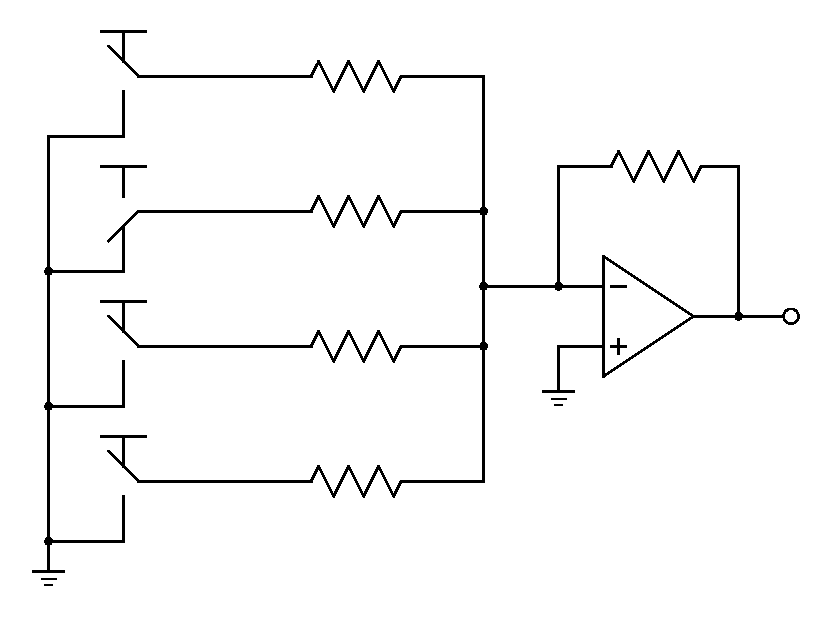
\includegraphics[scale=0.90]{DAC}
\caption{چار بِٹ کا عددی سے مماثل کار}
\label{شکل_حسابی_عددی_سے_مماثل_کار}
\end{figure}
آئیں اس دور کو حل کرتے ہیں۔
\begin{align*}
v_k=0\\
\frac{v_n-d_3}{R}+\frac{v_n-d_2}{2R}+\frac{v_n-d_1}{4R}+\frac{v_n-d_0}{8R}+\frac{v_n-v_o}{R'}=0\\
v_0=-\frac{R'}{8 R} \left(8 d_3+4d_2+2d_1+d_0 \right)
\end{align*}
جسے یوں بہتر طریقے سے لکھا جا سکتا ہے۔
\begin{align} \label{مساوات_حسابی_عددی_سے_مماثل_کار}
v_0=-\frac{R'}{8 R} \left(2^3 d_3+2^2 d_2+2^1 d_1+2^0 d_0 \right)
\end{align}

\موٹا{عددی سے مماثل کار} عددی\حاشیہب{digital} متغیرہ لیتے ہوئے اس کا مماثل\حاشیہب{analog} متغیرہ خارج کرتا ہے۔عددی متغیرات کو  \موٹا{دہری نظام اعداد}\فرہنگ{دہری نظام اعداد}\حاشیہب{binary number system} میں لکھا جاتا ہے۔\موٹا{دہری  نظام اعداد} کے دو ہی ہندسے ہیں یعنی \عددی{0} (صفر) اور \عددی{1} (ایک)۔ \عددی{0}کو \عددی{\SI{0}{\volt}} اور \عددی{1} کو \عددی{\SI{5}{\volt}} سے ظاہر کیا جاتا ہے۔\عددی{d_0} تا \عددی{d_3} کو \عددی{d_3 d_2 d_1 d_0} لکھتے ہوئے چار \موٹا{بِٹ}\فرہنگ{بِٹ}\فرہنگ{bit}\حاشیہب{bit} کا دہرا عدد حاصل ہوتا ہے۔یوں شکل میں دکھائی صورت
\begin{align*}
d_3 d_2 d_1 d_0 =1011_2
\end{align*}
کو ظاہر کرتی ہے جو کہ \موٹا{اعشاری نظام گنتی}\حاشیہب{decimal number system} میں  گیارہ \عددی{11_{10}} کے برابر ہے۔

اگر تمام داخلی \موٹا{دہرے ہندسے} صفر کر دیے جائیں تو  مساوات \حوالہ{مساوات_حسابی_عددی_سے_مماثل_کار} کے مطابق \موٹا{عددی سے مماثل کار} \عددی{v_o=\SI{0}{\volt}} خارج کرے گا جبکہ اگر تمام داخلی دہرے ہندسے ایک کر دیے جائیں یعنی انہیں \عددی{\SI{5}{\volt}} سے ظاہر کیا جائے تب دور
\begin{align*}
v_0&=-\frac{R'}{8 R} \left(2^3 \times 5+2^2 \times 5+2^1 \times 5+2^0 \times 5 \right)\\
&=-\frac{R'}{8 R} \left(2^3+2^2 +2^1 +2^0  \right) \times 5\\
&=-\frac{R'}{8 R} \left(8+4 +2 +1 \right) \times 5\\
&=-\frac{R'}{8 R}\times 75
\end{align*}  
خارج کرے گا۔

\عددی{R'} اور \عددی{R} کی قیمت سے درکار قیمت تعین کی جا سکتی ہے۔مثلاً \عددی{R'=\tfrac{8 R}{15}} رکھتے ہوئے مندرجہ بالا مساوات کے مطابق \موٹا{عددی سے مماثل کار} \عددی{v_o=\SI{-5}{\volt}} خارج کرے گا۔چونکہ \عددی{d_o} تا \عددی{d_3} کے چار ہندسوں پر مبنی دہرا عدد سولہ \عددی{16_{10}} مختلف قیمتیں ظاہر کر سکتا ہے لہٰذا \موٹا{عددی سے مماثل کار} صفر وولٹ تا منفی پانچ وولٹ سولہ مختلف قیمتیں خارج کر سکتا ہے۔

\موٹا{عددی سے مماثل کار} میں اسی طرز پر مزید داخلی اشارات  جوڑتے ہوئے زیادہ ہندسوں کا \موٹا{عددی سے مماثل کار} بنایا جاتا ہے۔ 

\ابتدا{مثال}
\عددی{R'=\tfrac{8 R}{15}} رکھتے ہوئے \عددی{d_3 d_2 d_1 d_0} کی قیمت \عددی{1010_2} ہونے کی صورت میں \موٹا{عددی سے مماثل کار} کتنی برقی دباو خارج کرے گا۔

حل:
\begin{align*}
v_0&=-\frac{R'}{8 R} \left(2^3 \times 5+2^2 \times 0+2^1 \times 5+2^0 \times 0 \right)\\
&=-\frac{R'}{8 R} \left(2^3+2^1  \right) \times 5\\
&=\SI{-3.333}{\volt}
\end{align*}  
\انتہا{مثال}

\جزوحصہ{یک سمتی  اندرونی داخلی انحرافی برقی دباو کا مسئلہ}

اگر کامل حسابی ایمپلیفائر کے دونوں داخلی سرے آپس میں جوڑ کر انہیں برقی زمین کے ساتھ جوڑا جائے، یعنی \عددی{v_k=v_n=0} کر دیا جائے، تو ہم توقع کرتے ہیں کہ اس کا خارجی   اشارہ صفر وولٹ کا ہو گا، یعنی \عددی{v_o = A_d v_d =0} ہو گا۔حقیقت میں ایسا نہیں ہوتا\حاشیہد{اس مسئلہ کے پیدا ہونے کی وجوہات پر  حصہ \حوالہ{حصہ_تفرقی_ایمپلیفائر_داخلی_انحرافی_برقی_دباو} میں تفصیلاً تبصرہ کیا جائے گا} اور عموماً اس طرح جڑا حسابی ایمپلیفائر مثبت یا منفی جانب \موٹا{لبریز}\فرہنگ{لبریز} پایا جاتا ہے۔ حسابی ایمپلیفائر کے \عددی{v_o} کو صفر وولٹ پر لانے کی خاطر حسابی ایمپلیفائر کے دونوں داخلی سروں کے مابین برقی دباو \عددی{V_{OS}} مہیا کرنا پڑتا ہے۔

	اس حقیقت کو یوں بھی بیان کیا جا سکتا ہے کہ حسابی ایمپلیفائر بناتے وقت پوری کوشش کے باوجود اسے کامل بنانا ناممکن ہوتا ہے اور اس میں کچھ کمی رہ جاتی ہے جس کی وجہ سے اس کا عمل یوں پایا جاتا ہے جیسے اس کے داخلی سروں کے مابین برقی دباو \عددی{V_{OS}}جڑی ہو۔اس خیالی برقی دباو \عددی{V_{OS}} کو ختم کرنے کی خاطر ہمیں اتنی ہی، مگر اُلٹ علامت والی، برقی دباو \عددی{V_{OS}} اس کے دونوں داخلی سروں کے مابین فراہم کرنی پڑتی ہے۔اس خیالی برقی دباو کو \موٹا{اندرونی داخلی انحرافی برقی دباو}\فرہنگ{اندرونی داخلی انحرافی برقی دباو}\فرہنگ{input offset voltage}\حاشیہب{input offset voltage}  کہتے ہیں۔شکل \حوالہ{شکل_انحرافی_برقی_دباو_اور_اس_کا_خاتمہ} میں اس کی وضاحت کی گئی ہے۔

	اندرونی داخلی انحرافی برقی دباو کی موجودگی غیر پسندیدہ حقیقت ہے جسے ختم کرنے کی تمام تر کوشش کی جاتی ہے۔حسابی ایمپلیفائر بنانے والے صنعت کار اپنے بنائے گئے حسابی ایمپلیفائر میں پائے جانے والے اندرونی داخلی انحرافی برقی دباو کے حدود کی معلومات فراہم کرتے ہیں۔یہ حدود عموماً \عددی{\SI{\mp 1}{\milli \volt}}  تا \عددی{\SI{\mp 5}{\milli \volt}} تک ہوتے ہیں۔ اندرونی داخلی انحرافی برقی دباو کی علامت نہیں بتلائی جاتی چونکہ قبل از استعمال اس کا جاننا ممکن نہیں ہوتا۔
\begin{figure}
\centering
\includegraphics[scale=0.90]{opampInputOffsetVoltage}
\caption{داخلی انحرافی برقی دباو اور اس کا خاتمہ}
\label{شکل_انحرافی_برقی_دباو_اور_اس_کا_خاتمہ}
\end{figure}
اندرونی داخلی انحرافی برقی دباو کا تخمینہ لگانے کی خاطر مثبت ایمپلیفائر استعمال کیا جا سکتا ہے۔شکل \حوالہ{شکل_داخلی_انحرافی_برقی_دباو_کی_پیمائش} میں اسے دکھایا گیا ہے۔اس شکل میں مثبت سرے کو برقی زمین کے ساتھ جوڑا گیا ہے۔مزاحمت \عددی{R_2} کی قیمت کو \عددی{R_1} کی قیمت سے اتنا بڑا رکھا جاتا ہے کہ خارجی  سرے پر چند وولٹ کی یک سمتی برقی دباو \عددی{V_{OS}} پایا جائے۔اس دور میں اندرونی داخلی انحرافی برقی دباو کو بطور داخلی اشارہ استعمال کیا گیا ہے۔اگر اس اندرونی داخلی انحرافی برقی دباو کی قیمت \عددی{V_{OS}} ہو تب مثبت ایمپلیفائر کے لئے یوں لکھا جا سکتا ہے۔
\begin{align}
V_{o}=\left (1+\frac{R_2}{R_1} \right ) V_{OS} =\frac{\left (R_1+R_2 \right )}{R_1} V_{OS}
\end{align}
%
\begin{figure}
\centering
\includegraphics[scale=0.90]{inputOffsetVoltageMeasurement}
\caption{داخلی انحرافی برقی دباو کی پیمائش}
\label{شکل_داخلی_انحرافی_برقی_دباو_کی_پیمائش}
\end{figure}
اس مساوات میں \عددی{V_{OS}} کے علاوہ تمام متغیرات ہمیں معلوم ہیں۔یوں ان سے\عددی{V_{OS}} حاصل کی جا سکتی ہے یعنی
\begin{align}
V_{OS}=\frac{R_1}{R_1+R_2} V_{o}
\end{align}
شکل \حوالہ{شکل_داخلی_انحرافی_برقی_دباو_سے_پاک_منفی_ایمپلیفائر} الف میں اندرونی داخلی انحرافی برقی دباو کے اثر کو ختم کر کے منفی ایمپلیفائر کا استعمال دکھایا گیا ہے۔ایسے ادوار میں \عددی{R_3} اور\عددی{R_5} کی قیمتیں کئی کلو اُوہم  \عددیء{\si{\kilo \ohm}} ہوتی ہیں جبکہ متغیر مزاحمت \عددی{R_4} کی قیمت اتنی رکھی جاتی ہے کہ اس کے درمیانی پنیا سے قابل حصول برقی دباو استعمال کردہ حسابی ایمپلیفائر کے اندرونی داخلی انحرافی برقی دباو \عددی{V_{OS}} کے حدود سے قدر زیادہ ہو۔ایسے متغیر مزاحمت پر پیچ نسب ہوتا ہے جسے گھماتے ہوئے حسابی ایمپلیفائر کے خارجی اشارے \عددی{V_o} کو صفر وولٹ کرتے ہوئے اندرونی داخلی انحرافی برقی دباو کے اثر کو ختم کیا جاتا ہے۔
\begin{figure}
\centering
\includegraphics[scale=0.90]{invertingAmplifierWithInputOffsetVoltageEliminated}
\caption{داخلی انحرافی برقی دباو سے پاک، منفی ایمپلیفائر}
\label{شکل_داخلی_انحرافی_برقی_دباو_سے_پاک_منفی_ایمپلیفائر}
\end{figure}

%============================
\ابتدا{مثال}
اگر شکل \حوالہ{شکل_داخلی_انحرافی_برقی_دباو_سے_پاک_منفی_ایمپلیفائر} الف میں
\begin{align*}
V_{CC} =\SI{12}{\volt} \hspace{1cm} V_{EE}=\SI{-12}{\volt} \hspace{1cm} V_{OS}=\SI{2}{\milli \volt}
\end{align*}
ہیں۔داخلی انحرافی برقی دباو کے خاتمے کے لئے درکار مزاحمت \عددیء{R_3}، \عددی{R_4} اور \عددی{R_5} منتخب کریں۔

حل:	چونکہ داخلی انحرافی برقی دباو کی قیمت معلوم ہونے کے باوجود اس کا رخ معلوم نہیں ہوتا لہٰذا ہمیں ان مزاحمت کو یوں منتخب کرنا ہو گا کہ \عددی{R_4} تبدیل کرتے ہوئے ہم \عددی{\SI{-2}{\milli \volt}} تا\عددی{\SI{+2}{\milli \volt}}  یعنی کُل \عددی{\SI{4}{\milli \volt}} کی تبدیلی حاصل کر سکیں۔ہم \عددی{R_3=R_5=\SI{100}{\kilo \ohm}}لیتے ہوئے \عددی{R_4} کی قیمت حاصل کرتے ہیں۔
\begin{align*}
 \left(+12-(-12) \right ) \times \left (\frac{R_4}{R_3+R_4+R_5} \right )&=0.004\\
 24 \times \left ( \frac{R_4}{200000+R_4} \right )&=0.004\\
 R_4 &= \SI{33}{\ohm}
\end{align*}
ہم اس سے قدر زیادہ مزاحمت منتخب کرتے ہیں مثلاً \عددی{R_4 =\SI{100}{\ohm}}۔

آئیں دیکھیں کہ ان قیمتوں سے \عددی{v_k} میں کن حدود کے مابین تبدیلی ممکن ہے۔\عددی{R_4} کے متغیر سرے کو ایک جانب پورا گھما کر شکل  الف     میں دکھایا گیا ہے۔اس صورت میں کرچاف کے قانون برائے برقی رو کی مدد سے ہم لکھ سکتے ہیں
\begin{align*}
\frac{v_k-V_{CC}}{R_3}+\frac{v_k-V_{EE}}{R_4+R_5}=0\\
\frac{v_k-12}{100000}+\frac{v_k+12}{100+100000}=0\\
v_k=\SI{5.99}{\milli \volt}
\end{align*}
اسی طرح اگر \عددی{R_4} کو دوسری جانب پورا گھمایا جائے تب
\begin{align*}
\frac{v_k-V_{CC}}{R_3+R_4}+\frac{v_k-V_{EE}}{R_5}=0\\
\frac{v_k-12}{100000+100}+\frac{v_k+12}{100000}=0\\
v_k=-\SI{5.99}{\milli \volt}
\end{align*}
حاصل ہوتا ہے۔موجودہ مثال میں حسابی ایمپلیفائر کا داخلی انحرافی برقی دباو \عددی{\SI{-2}{\milli \volt}} تا\عددی{\SI{+2}{\milli \volt}} کے مابین کہیں پر بھی ہو سکتا ہے۔حسابی ایمپلیفائر کا داخلی اشارہ \عددی{v_s=0} رکھتے ہوئے اس  کے خارجی اشارے \عددی{v_o}  پر نظر رکھ کر \عددی{R_4} کو اس مقام پر لایا جاتا ہے جہاں \عددی{v_o=0} حاصل ہو۔\عددی{R_4} کو اسی قیمت پر پکا چھوڑ دیا جاتا ہے۔
\انتہا{مثال}

شکل \حوالہ{شکل_داخلی_انحرافی_برقی_دباو_سے_پاک_ایمپلیفائر} میں داخلی انحرافی برقی دباو سے پاک منفی اور مثبت ایمپلیفائر دکھائے گئے ہیں۔ان ادوار میں \عددیء{R_3=\SI{100}{\ohm}}، \عددیء{R_4=\SI{150}{\kilo \ohm}}، \عددیء{R_5=\SI{50}{\kilo \ohm}}، \عددی{V_{+}=\SI{12}{\volt}} اور  \عددی{V_{-}=\SI{-12}{\volt}} کی صورت میں \عددی{\SI{\pm 8}{\milli \volt}} کے \موٹا{داخلی انحرافی برقی دباو} کا خاتمہ ممکن ہو گا۔ 
\begin{figure}
\centering
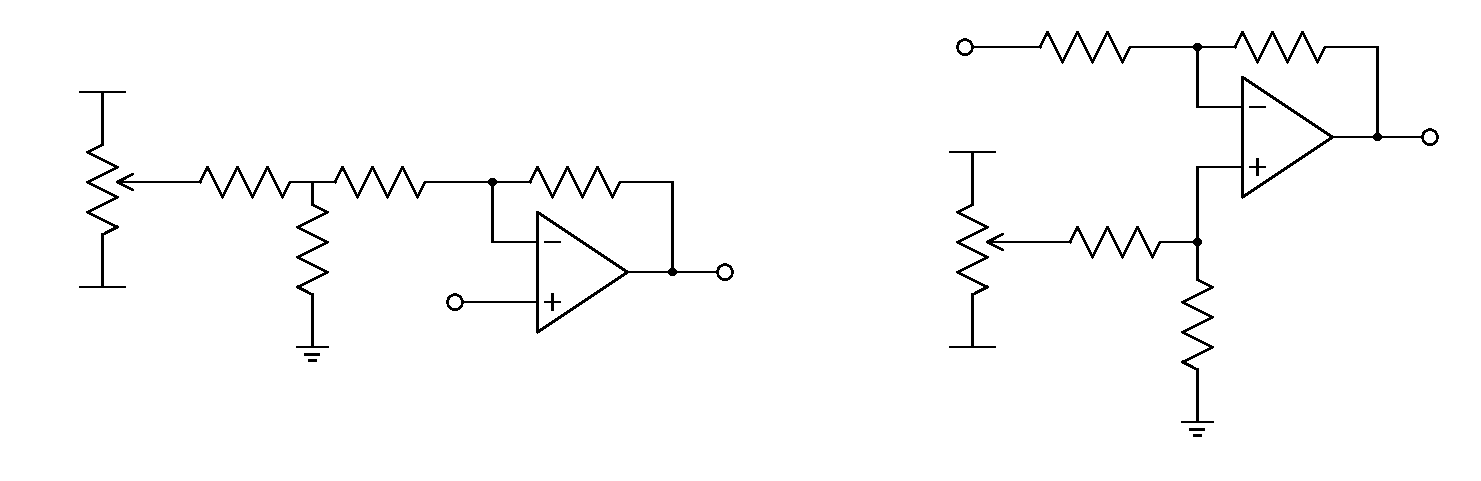
\includegraphics[scale=0.90]{opampInputOffsetVoltageElimination}
\caption{داخلی انحرافی برقی دباو سے پاک ایمپلیفائر}
\label{شکل_داخلی_انحرافی_برقی_دباو_سے_پاک_ایمپلیفائر}
\end{figure}
%=================
\جزوحصہ{داخلی برقی رو کا مسئلہ} \شناخت{حصہ_حسابی_داخلی_برقی_رو}

اگرچہ حسابی ایمپلیفائر کی داخلی برقی رو  \عددی{I_B} کی قیمت عموماً قابل نظر انداز ہوتی ہے البتہ کبھی کبھار نہایت حساس یا باریک اشارات کی قیمت بھی\عددی{I_B} کے لگ بھگ ہوتی ہے۔ایسی صورت میں \عددی{I_B}کو نظر انداز کرنا ممکن نہیں ہوتا۔اس طرح کے مجبوری کے علاوہ بھی ادوار بناتے وقت اگر \عددی{I_B} کو مد نظر رکھا جائے تو کچھ حرج نہیں۔داخلی برقی رو یک سمتی نوعیت کی ہوتی ہے۔حسابی ایمپلیفائر کے درست کارکردگی کے لئے یہ ضروری ہے کہ اس کے دونوں داخلی سروں  پر یک سمتی برقی رو کے لئے راستہ موجود ہو۔آئیں دیکھتے ہیں کہ اس \عددی{I_B} کے بارے میں عموماً کیا کیا جاتا ہے۔

حسابی ایمپلیفائر کی اندرونی ساخت کی وجہ سے اس کے داخلی سروں پر یک سمتی برقی رو درکار ہوتی ہے۔مزید یہ کہ دونوں داخلی سروں پر برقی رو کا رخ ایک ہی سمت میں ہوتا ہے۔اگر کسی ایک قسم کے ایمپلیفائر میں برقی رو کا رخ داخلی سروں پر اندر کی جانب ہو تو کسی دوسرے قسم کے ایمپلیفائر میں دونوں یک سمتی داخلی برقی رو کا رخ باہر  کی جانب ہو سکتا ہے۔اس داخلی برقی رو جسے \موٹا{داخلی میلان برقی رو}\فرہنگ{داخلی میلان برقی رو}\فرہنگ{input bias current}\حاشیہب{input bias current} کہتے ہیں کے مقدار کا دارومدار ایمپلیفائر کی ساخت پر ہوتا ہے۔
\begin{figure}
\centering
\includegraphics[scale=0.90]{opampInputBiasCurrent}
\caption{داخلی برقی رو کا مسئلہ}
\label{شکل_داخلی_برقی_رو_کا_مسئلہ}
\end{figure}
شکل \حوالہ{شکل_داخلی_برقی_رو_کا_مسئلہ} الف میں مستحکم کار دکھایا گیا ہے جہاں حسابی ایمپلیفائر کے داخلی برقی رو \عددی{I_{B1}} اور\عددی{I_{B2}} کو پیدا کار مستقل برقی رو\حاشیہب{constant current source}  تصور کیا گیا ہے۔یک سمتی داخلی اشارہ \عددی{V_S} کی قیمت صفر ہونے کی صورت میں  شکل  الف     حاصل ہوتا  ہے ۔مستحکم کار کی خاصیت یہ ہے کہ یہ داخلی اشارہ کو بغیر تبدیلی خارج کرتا ہے۔یوں ہم توقع رکھتے ہیں کہ \عددی{V_S=0} کی صورت میں \عددی{V_O=0} ہو گا مگر ایسا نہیں ہوتا۔شکل  الف     پر غور کرنے سے معلوم ہوتا ہے کہ داخلی برقی رو کی وجہ سے
\begin{align*}
V_K=-I_{B2} R
\end{align*}
حاصل ہوتا ہے۔ \عددی{V_N=V_K} ہونے سے
\begin{align} \label{مساوات_انحرافی_رو_سے_پیدا_دباو}
V_O=-I_{B2}R
\end{align}
حاصل ہو گا۔جیسا کہ پہلے ذکر ہوا، چونکہ عام حالات میں \موٹا{داخلی میلان برقی رو} کی قیمت نہایت کم ہوتی ہے لہٰذا اس برقی رو کو عموماً نظر انداز کرنا ممکن ہوتا ہے۔اس وقت ہم کوئی ایسی ترکیب جاننا چاہیں گے کہ نا قابل نظر انداز \موٹا{داخلی میلان برقی رو} کی صورت میں یہ دور \عددی{V_O=0}خارج کرے۔

	شکل \حوالہ{شکل_داخلی_برقی_رو_کے_مسئلے_کا_حل} میں مستحکم کار کو ذرا تبدیل کرتے ہوئے اس میں مزاحمت \عددی{R_1} شامل کیا گیا ہے۔مستحکم کار کی کارکردگی ایسا کرنے سے ہرگز متاثر نہیں ہوتی۔اس دور میں بھی
\begin{align*}
V_K=-I_{B2}R
\end{align*}
اور
\begin{align*}
V_N=V_K=-I_{B2}R
\end{align*}
حاصل ہوتا ہے۔البتہ \عددی{R_1} پر اُوہم کے قانون سے
\begin{align*}
V_O-V_N=I_{B1}R_1
\end{align*}
لکھا جا سکتا ہے جس سے
\begin{align*}
V_O=V_N+I_{B1}R_1
\end{align*}
حاصل ہوتا ہے۔اگر دونوں \موٹا{داخلی میلان برقی رو} کے قیمتیں برابر ہوں ( \عددی{I_{B1}=I_{B2}=I_B}) تب ہم اس مساوات کو یوں لکھ سکتے ہیں۔
\begin{align*}
V_O=-I_B R +I_B R_1
\end{align*}
دور میں
\begin{align}
R_1=R
\end{align}
لینے سے\عددی{V_O=0} حاصل ہوتا ہے یعنی
\begin{align*}
V_O=-I_B R +I_B R=0
\end{align*}

پس ہم نے دیکھا کہ دور میں دونوں دخول پر یک سمتی برقی رو کے لئے برابر مزاحمت نسب کرنے سے \موٹا{داخلی میلان برقی رو} کا مسئلہ حل ہو جاتا ہے۔
\begin{figure}
\centering
\includegraphics[scale=0.90]{biasCurrentEffectElimination}
\caption{داخلی برقی رو کے مسئلے کا حل}
\label{شکل_داخلی_برقی_رو_کے_مسئلے_کا_حل}
\end{figure}

اگر \عددی{R_1=R}لیتے ہوئے اس حقیقت کو مد نظر رکھا جائے کہ دونوں داخلی برقی رو کے قیمتیں برابر نہیں ہوتیں تو اس صورت میں گزشتہ مساوات سے
\begin{align} \label{مساوات_انحرافی_رو_سے_پیدا_درست_دباو}
V_O=-I_{B2}R+I_{B1}R=\left (I_{B1}-I_{B2} \right )R
\end{align}
حاصل ہوتا ہے۔اگرچہ اس صورت میں \عددی{V_O=0} حاصل نہیں ہو گا مگر چونکہ
\begin{align*}
\abs{I_{B1}-I_{B2}} << I_B
\end{align*} 
ہوتا ہے لہٰذا مساوات \حوالہ{مساوات_انحرافی_رو_سے_پیدا_درست_دباو} سے حاصل \عددی{V_O} کی قیمت مساوات \حوالہ{مساوات_انحرافی_رو_سے_پیدا_دباو}  سے حاصل \عددی{V_O} کی قیمت سے زیادہ بہتر (یعنی کم) ہے۔
%=========
\ابتدا{مثال}
منفی ایمپلیفائر میں مسئلہ داخلی برقی دباو کی نشاندہی کریں اور اس سے نپٹنے کا حل دریافت کریں۔

حل:	شکل \حوالہ{شکل_منفی_ایمپلیفائر} میں منفی ایمپلیفائر دکھایا گیا ہے جس میں داخلی اشارہ کی قیمت صفر کرنے سے شکل  \حوالہ{شکل_منفی_ایمپلیفائر_اور_داخلی_برقی_رو_کا_مسئلہ} الف حاصل ہوتا ہے۔
\begin{figure}
\centering
\includegraphics[scale=0.90]{invertingAmplifierWithBiasCurrentEffectEliminated}
\caption{منفی ایمپلیفائر میں مسئلہ داخلی برقی رو اور اس کا حل}
\label{شکل_منفی_ایمپلیفائر_اور_داخلی_برقی_رو_کا_مسئلہ}
\end{figure}
شکل-الف میں مثبت داخلی سرا  برقی زمین کے ساتھ جڑا ہے لہٰذا \عددی{V_K=0} ہے اور یوں \عددی{V_N=V_K=0} ہو گا۔\عددی{V_N=0} ہونے کی وجہ سے\عددی{I_{R1}=0} ہو گا اور یوں منفی داخلی سرے  کی داخلی برقی رو تمام کی تمام مزاحمت \عددی{R_2} سے گزرے گی یعنی \عددی{I_{R2}=I_{B1}}ہو گا۔مزاحمت \عددی{R_2} پر اُوہم کے قانون سے \عددی{V_O} یوں حاصل ہوتا ہے۔
\begin{gather} \label{مساوات_انحرافی_دباو_کا_خاتمہ_ب}
\begin{aligned}
& V_O-V_N=I_{R2}R_2\\
& V_O =V_N +I_{R2}R_2\\
& V_O = 0 +I_{B1}R2\\
& V_O=I_{B1} R_2
\end{aligned}
\end{gather}
شکل \حوالہ{شکل_منفی_ایمپلیفائر_اور_داخلی_برقی_رو_کا_مسئلہ} ب میں مثبت داخلی سرے  سے برقی زمین تک مزاحمت \عددی{R} جوڑ کر داخلی برقی رو کے مسئلے کو حل کرنے کی کوشش کی گئی ہے۔جیسا شکل میں دکھایا گیا ہے \عددی{I_R=I_{B2}} ہونے کی وجہ سے \عددی{V_K=-I_{B2}R} ہو گا۔یوں منفی داخلی سرے  پر بھی اتنا ہی برقی دباو ہو گا (یعنی \عددی{V_N=V_K=-I_{B2}R})۔مزاحمت \عددی{R_1} کا بایاں سرا برقی زمین پر ہے جب کہ اس کا دایاں سرے پر منفی برقی دباو ہے لہٰذا اس میں بائیں سرے سے دائیں سرے کی جانب برقی رو گزرے گا
\begin{align*}
I_{R1}=\frac{R}{R_1}I_{B2}
\end{align*}
 منفی داخلی سرے  پر کرچاف کے قانون برائے برقی رو کی مدد سے \عددی{I_{R2}} یوں حاصل کیا جا سکتا ہے۔
\begin{align*}
&I_{R1}+I_{R2}=I_{B1}\\
&\frac{R}{R_1}I_{B2}+I_{R2}=I_{B1}\\
&I_{R2}=I_{B1}-\frac{R}{R_1}I_{B2}
\end{align*}
مزاحمت \عددی{R_2} پر اُوہم کا قانون استعمال کرتے ہوئے \عددی{V_O} حاصل کرتے ہیں۔
\begin{gather} \label{مساوات_انحرافی_دباو_کا_خاتمہ_الف}
\begin{aligned}
& V_O-V_N=I_{R2}R_2\\
& V_O=V_N+I_{R2}R_2\\
& V_O=-I_{B2}R+\left (I_{B1}-\frac{R}{R_1}I_{B2} \right ) R_2
\end{aligned}
\end{gather}
اگر دونوں داخلی میلان برقی رو کی قیمتیں برابر ہوں یعنی \عددی{I_{B1}=I_{B2}} تب اس مساوات سے حاصل ہوتا ہے۔
\begin{gather}
\begin{aligned}
 V_O&=-I_B R + \left (I_B-\frac{R}{R_1}I_B \right ) R_2\\
&=I_B \left (-R+R_2-\frac{R R_2}{R_1} \right ) 
\end{aligned}
\end{gather}
ہم چاہتے ہیں کہ داخلی میلان برقی رو کی وجہ سے کسی قسم کا خارجی برقی دباو پیدا نہ ہو۔اس مساوات میں\عددی{V_O=0}  استعمال کرتے ہوئے ہم \عددی{R} کی وہ قیمت دریافت کر سکتے ہیں جس سے ایسا ممکن ہو یعنی
\begin{align}
R=\frac{R_1 R_2}{R_1+R_2}
\end{align}
پس منفی ایمپلیفائر کے مثبت داخلی سرے  اور برقی زمین کے درمیان متوازی جڑے \عددی{R_1} اور \عددی{R_2} کے برابر مزاحمت نسب کرنے سے داخلی  میلان برقی رو کا مسئلہ حل ہو جاتا ہے۔

اگر دونوں داخلی میلان برقی رو برابر نہ ہوں تب مساوات \حوالہ{مساوات_انحرافی_دباو_کا_خاتمہ_الف}  میں 
\begin{align*}
R=\frac{R_1 R_2}{R_1+R_2}
\end{align*}
لیتے ہوئے
\begin{align}
V_O=\left (I_{B1}-I_{B2} \right )R_2
\end{align}
حاصل ہوتا ہے۔یوں اس صورت میں اگرچہ داخلی میلان برقی رو کا مسئلہ پوری طرح حل نہیں ہوتا لیکن مساوات \حوالہ{مساوات_انحرافی_دباو_کا_خاتمہ_ب}  کے ساتھ موازنہ کرنے سے (چونکہ \عددی{I_{B1}>>\abs{I_{B1}-I_{B2}}} ہے ) ہم دیکھتے ہیں کہ \عددی{V_O}  میں خاطر خواہ کمی آتی ہے۔

\انتہا{مثال}

%=================================

ہم دیکھتے ہیں کہ حسابی ایمپلیفائر کے دونوں داخلی سروں پر یک سمتی میلان برقی رو کو برقی زمین تک پہنچنے کی خاطر برابر مزاحمت فراہم کرنے سے داخلی برقی رو کا مسئلہ حل ہوتا ہے۔یہاں یک سمتی میلان برقی رو کے راستے کی بات کی گئی نہ کہ بدلتے برقی رو کے راستے کی۔اس بات کی وضاحت شکل \حوالہ{شکل_مسئلہ_داخلی_برقی_رو_کے_چند_مثال}    کی مدد سے کرتے ہیں۔یاد رہے کہ کپیسٹر میں یک سمتی برقی رو نہیں گزر سکتا اور یہ بالکل لامحدود مزاحمت کی طرح کردار ادا کرتا ہے۔شکل  \حوالہ{شکل_منفی_ایمپلیفائر_اور_داخلی_برقی_رو_کا_مسئلہ} الف میں منفی ایمپلیفائر دکھایا گیا ہے جس کا عمومی طور پر مثبت داخلی سرا برقی زمین کے ساتھ جڑا ہوتا ہے۔منفی داخلی سرے  کے یک سمتی میلان  برقی رو کا برقی زمین تک راستہ \عددی{R_2} ہے اور یوں مثبت داخلی سرے  اور برقی زمین کے درمیان \عددی{R=R_2} جوڑ کر داخلی میلان برقی رو کا مسئلہ حل کیا گیا ہے۔شکل \حوالہ{شکل_منفی_ایمپلیفائر_اور_داخلی_برقی_رو_کا_مسئلہ} ب میں مثبت ایمپلیفائر دکھایا گیا ہے۔یہاں اشارہ کو کپیسٹر کے ذریعہ ایمپلیفائر کے ساتھ جوڑا گیا ہے جس سے اس داخلی سرے  کے میلان برقی رو کو برقی زمین تک راستہ میسر نہیں ہو گا اور یوں یہ ایمپلیفائر کام کرنے سے قاصر ہے۔اس کی صحیح کارکردگی کے لئے ضروری ہے کہ اس داخلی سرے  سے برقی زمین تک یک سمتی میلان برقی رو کے لئے راستہ موجود ہو۔چونکہ منفی  داخلی سرے  کے یک سمتی میلان برقی رو کا برقی زمین تک راستہ \عددی{R_1} اور \عددی{R_2} کے ذریعہ ہے اور یک سمتی میلان برقی رو کے نقطہ نظر سے یہ دونوں مزاحمت متوازی جڑے ہیں لہٰذا مثبت  داخلی سرے  اور زمین کے درمیان مزاحمت
\begin{figure}
\centering
\includegraphics[scale=0.90]{inputBiasCurrentExamplesA}
\caption{مسئلہ داخلی برقی رو کے چند مثالیں اور یک سمتی برقی رو کا برقی زمین تک رسائی کا راستہ}
\label{شکل_مسئلہ_داخلی_برقی_رو_کے_چند_مثال}
\end{figure}
%
\begin{align*}
R=\frac{R_1 R_2}{R_1+R_2}
\end{align*}
نسب کر کے اس داخلی سرے  کے یک سمتی میلان برقی رو کو زمین تک راستہ فراہم کیا جاتا ہے اور ساتھ ہی ساتھ مسئلہ داخلی میلان برقی رو کو بھی حل کیا جاتا ہے۔یہاں یہ بتلانا ضروری ہے کہ مثبت داخلی سرے  اور زمین کے درمیان مزاحمت \عددی{R} نسب کرنے سے اس داخلی سرے  کا داخلی مزاحمت کم ہوتا ہے جو کہ عموماً قابل برداشت نہیں ہوتا۔



\حصہ{موازنہ کار}
شکل \حوالہ{شکل_حسابی_موازنہ_کار} الف کے حسابی ایمپلیفائر میں \عددی{v_2  > v_1} کی صورت میں \عددی{v_o} مکمل مثبت یعنی \عددی{V_{CC}} پر ہو گا جبکہ \عددی{v_2 < v_1} کی صورت میں \عددی{v_o} مکمل منفی یعنی \عددی{V_{EE}} پر ہو گا۔حسابی ایمپلیفائر داخلی اشارات کا موازنہ کرتے ہوئے \عددی{V_{CC}} یا  \عددی{V_{EE}} خارج کرتا ہے۔یہ عمل نہایت اہم ہے اور اس عمل کی رفتار تیز تر درکار ہوتی ہے۔\موٹا{موازنہ کار}\فرہنگ{موازنہ کار}\فرہنگ{comparator}\حاشیہب{comparator} ایسا مخلوط دور ہے جسے خاص اسی مقصد کے لئے تخلیق دیا گیا ہے۔


\begin{figure}
\centering
\includegraphics[scale=0.90]{comparator}
\caption{موازنہ کار}
\label{شکل_حسابی_موازنہ_کار}
\end{figure}

\موٹا{موازنہ کار} کی علامت وہی ہے جو حسابی ایمپلیفائر کی ہے۔حسابی ایمپلیفائر مثبت یا منفی اشارہ خارج کر سکتا ہے جبکہ  \موٹا{موازنہ کار} داخلی اشارات کا موازنہ کرتے ہوئے  دو مختلف صورت اختیار کر سکتا ہے۔ایک صورت میں یہ منقطع ہو جاتا ہے جبکہ دوسری صورت میں یہ مقرر برقی دباو خارج کرتا ہے جو عموماً  \عددی{\SI{0}{\volt}} یا \عددی{V_{EE}} ہوتا ہے۔

\موٹا{موازنہ کار}  کی کارکردگی کو شکل  الف     میں دکھایا گیا ہے جہاں اس کے ممکنہ خارجی صورت \موٹا{منقطع} اور \عددی{\SI{0}{\volt}} ہیں۔\عددی{v_2 > v_1} کی صورت میں سوئچ منقطع رہتا ہے جبکہ \عددی{v_2 < v_1} کی صورت میں سوئچ چالو ہو کر خارجی سرے  کو برقی زمین کے ساتھ جوڑتا ہے۔خارجی سرے اور \عددی{V_{CC}} کے درمیان مزاحمت \عددی{R_{\textup{اوپر کھینچ}}} جوڑنے سے منقطع صورت میں \عددی{v_o=V_{CC}} حاصل کیا جا سکتا ہے۔

آئیں \موٹا{موازنہ کار} کے استعمال کی ایک مثال دیکھیں۔

\ابتدا{مثال}
 اس مثال میں چالو مشین کے درجہ حرارت اور اس میں میکانی دباو پر نظر رکھا جاتا ہے۔اگر ان میں کوئی ایک یا دونوں مقررہ حدف سے تجاوز کریں تو مشین کو منقطع کر دیا جاتا ہے۔مشین اس وقت تک چالو رہتا ہے جب تک اسے چالو رکھنے والا \عددی{\SI{5}{\volt}} کا اشارہ ملتا رہے۔مشین اسی دم منقطع ہو جاتا ہے جب اسے منقطع کرنے والا \عددی{v_o=\SI{0}{\volt}} کا اشارہ ملے۔منقطع کر دینے والے اشارے کو تیر کے نشان سے دکھایا گیا ہے۔

شکل \حوالہ{شکل_حسابی_موازنہ_کار_مقررہ_حدف} میں  دو \موٹا{موازنہ کار} متوازی جوڑے گئے ہیں۔نچلے \موٹا{موازنہ کار} کے منفی داخلی سرے  پر \تحریر{TMP37}\حاشیہب{Analog Devices اس مخلوط دور کو بناتے ہیں۔} کا خارجی اشارہ جوڑا گیا ہے جسے شکل میں \موٹا{درجہ حرارت} کہا گیا ہے۔\تحریر{TMP37} ایسا مخلوط دور ہے جو درجہ حرارت کے راست متناسب برقی دباو خارج کرتا ہے۔\عددی{\SI{0}{\celsius}} پر \عددی{\SI{0}{\volt}} اور \عددی{\SI{100}{\celsius}} پر  یہ \عددی{\SI{1}{\volt}} خارج کرتا ہے۔اس کو \عددی{\SI{5}{\volt}} کی درکار طاقت مہیا کی گئی ہے۔اسی \موٹا{موازنہ کار} کے مثبت داخلی سرے  پر قابل تبدیل مزاحمت نسب کی گئی ہے۔قابل تبدیل مزاحمت پر نسب پیچ کو گھماتے ہوئے \موٹا{موازنہ کار} کے مثبت داخلی سرے  پر \عددی{\SI{0}{\volt}} تا \عددی{\SI{5}{\volt}} برقی دباو دیا  جا سکتا ہے جسے  شکل میں \موٹا{مقررہ درجہ حرارت} کہا گیا ہے۔\موٹا{مقررہ درجہ حرارت} کو \عددی{\SI{0.5}{\volt}} پر رکھا گیا ہے۔\عددی{\SI{50}{\celsius}} پر \تحریر{TMP37} اشاریہ پانچ \عددی{\SI{0.5}{\volt}} خارج کرے گا۔

موازنہ کار اس وقت تک منقطع رہے گا جب تک درجہ حرارت \عددی{\SI{50}{\celsius}} سے کم رہے۔جیسے ہی درجہ حرارت اس حدف سے تجاوز کرے، موازنہ کار  \عددی{v_o=\SI{0}{\volt}} خارج کرتے ہوئے مشین کو منقطع کر دیگا۔
\begin{figure}
\centering
\includegraphics[scale=0.90]{comparatorExample}
\caption{موازنہ کار کی مثال}
\label{شکل_حسابی_موازنہ_کار_مقررہ_حدف}
\end{figure}

شکل میں دکھائے دوسرے موازنہ کار کو بھی اسی طرح استعمال کیا گیا ہے۔اس کا مثبت داخلی سرے کو مقررہ میکانی دباو کے حدف پر رکھا جاتا ہے جبکہ اس کے منفی داخلی سرے  کو مشین میں پائے جانے والے میکانی دباو کا اشارہ مہیا کیا جاتا ہے۔جیسے ہی میکانی دباو مقررہ حدف سے تجاوز  کرے، موازنہ کار خارجی اشارے \عددی{v_o} کو نیچے کھینچ کر برقی زمین \عددی{\SI{0}{\volt}} پر لاتے ہوئے مشین کو منقطع کر دیگا۔

آپ دیکھ سکتے ہیں کہ دونوں موازنہ کار خارجی اشارے کو صرف برقی زمین پر لانے کی صلاحیت رکھتے ہیں۔

اسی طرح مزید موازنہ کار متوازی جوڑتے ہوئے دیگر متغیرات پر نظر رکھی جا سکتی ہے۔
\انتہا{مثال}
%===============================
%=================================
\newpage
\حصہء{سوالات}

\ابتدا{سوال}
شکل \حوالہ{شکل_حسابی_منفی_اقسام} میں
\begin{align*}
V_{CC}=\SI{12}{\volt} \hspace{5mm} V_{EE}=\SI{-12}{\volt} \hspace{5mm} v_s=\SI{0.5}{\volt}\\
R_1=\SI{10}{\kilo \ohm} \hspace {5mm} R_2=\SI{200}{\kilo \ohm} \hspace{5mm} R_3=\SI{10}{\kilo \ohm}
\end{align*}
ہیں۔
\begin{itemize}
\item
کامل حسابی ایمپلیفائر تصور کرتے ہوئے ان تمام ادوار کے داخلی مزاحمت اور خارجی اشارے  حاصل کریں۔
\item
غیر کامل حسابی ایمپلیفائر تصور کرتے ہوئے دوبارہ حل کریں۔غیر کامل حسابی ایمپلیفائر کے جزو
\begin{align*}
A=\num{60000} \hspace{5mm} R_i=\SI{100}{\mega \ohm} \hspace{5mm} R_o=\SI{200}{\ohm}
\end{align*}
ہیں۔
\end{itemize}
%
\begin{figure}
\centering
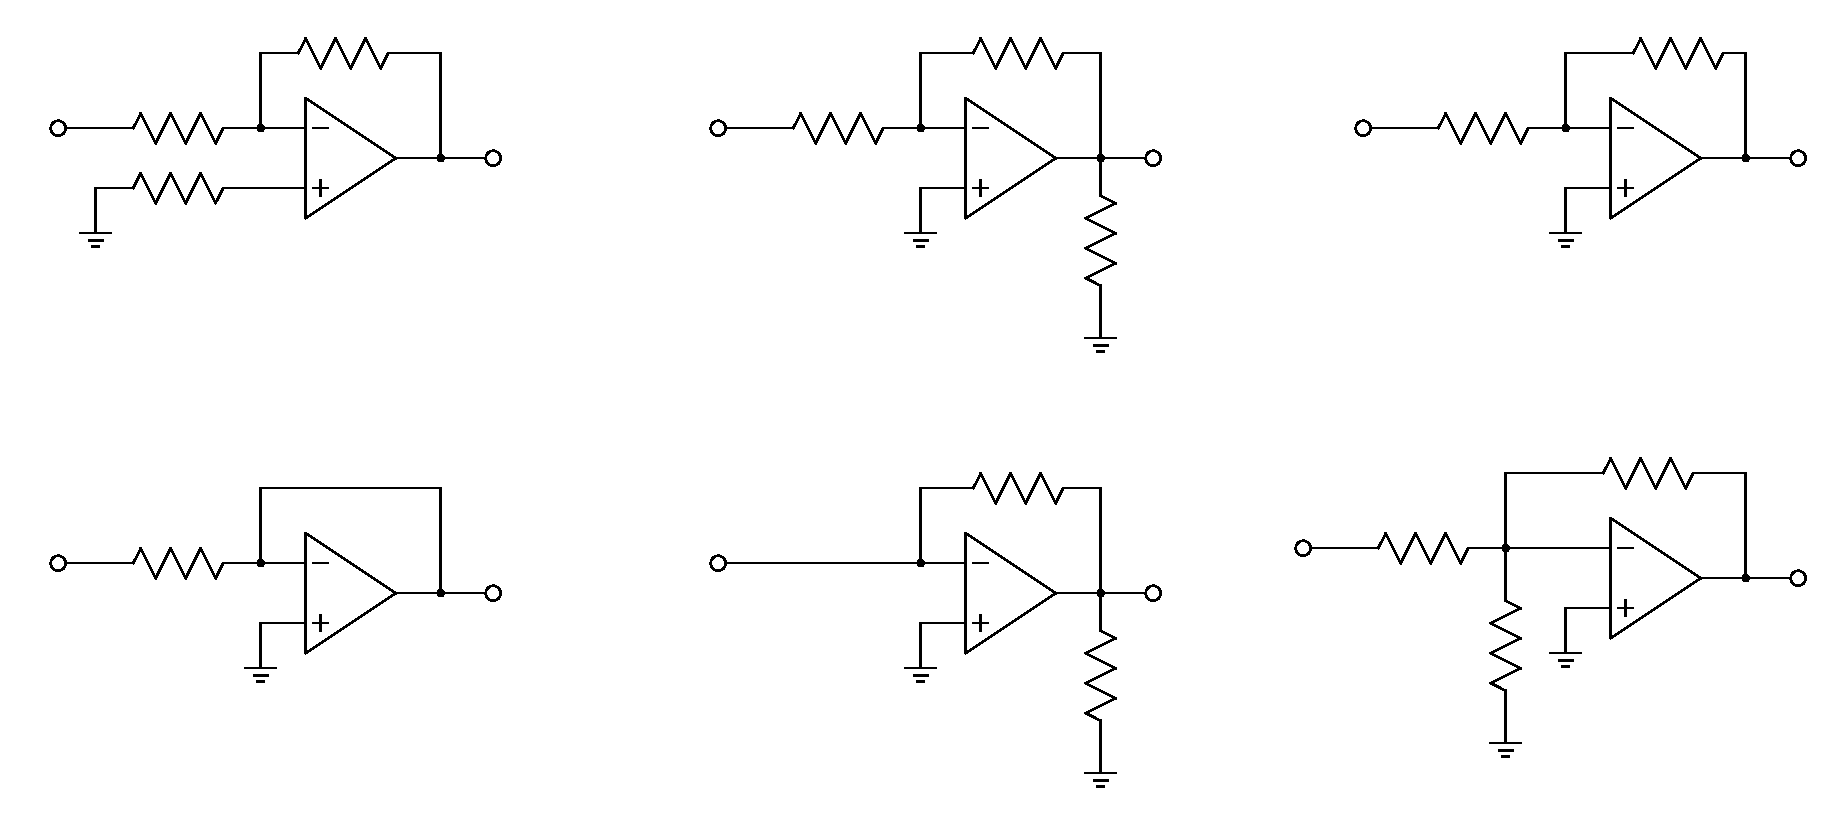
\includegraphics[scale=0.90]{questionsOpampInvertingVariations}
\caption{حسابی منفی ایمپلیفائر کے سوالات}
\label{شکل_حسابی_منفی_اقسام}
\end{figure}

جوابات:
\begin{itemize}
\item
داخلی مزاحمت: \عددیء{\SI{10}{\kilo \ohm}}، \عددیء{\SI{10}{\kilo \ohm}}، \عددیء{\SI{10}{\kilo \ohm}}، \عددیء{\SI{10}{\kilo \ohm}}، \عددیء{\SI{0}{ \ohm}} اور \عددی{\SI{10}{\kilo \ohm}} 
خارجی اشارہ: \عددیء{\SI{-10}{\volt}}، \عددیء{\SI{-10}{\volt}}، \عددیء{\SI{-10}{\volt}}، \عددیء{\SI{-10}{\volt}}، \عددیء{\SI{-12}{\volt}} اور \عددیء{\SI{0}{\volt}}
\end{itemize}
\انتہا{سوال}
%==================================
\ابتدا{سوال} \شناخت{سوال_سادہ_منفی_ایمپلیفائر}
کامل حسابی ایمپلیفائر تصور کرتے ہوئے \عددی{\SI{10}{\mega \ohm}} سے کم مزاحمتوں کے استعمال سے  صفحہ \حوالہصفحہ{شکل_منفی_ایمپلیفائر} پر دیے شکل \حوالہ{شکل_منفی_ایمپلیفائر} کے طرز پر منفی حسابی ایمپلیفائر تخلیق دیں۔ 
\begin{itemize}
\item
 \عددی{A_v=\SI{-25}{\volt\per \volt}} کی صورت میں \عددی{R_1}، \عددی{R_2} اور زیادہ سے زیادہ ممکنہ داخلی مزاحمت کیا ہو گی۔ 
\item
\عددی{A_v=\SI{-1000}{\volt\per \volt}} کی صورت میں زیادہ سے زیادہ ممکنہ داخلی مزاحمت کیا ہو گی۔ 
\end{itemize}

جوابات: \عددیء{R_1=\SI{400}{\kilo \ohm}}، \عددیء{R_2=\SI{10}{\mega \ohm}}، \عددیء{R_{\textup{داخلی}}=\SI{400}{\kilo \ohm}} اور  \عددیء{R_{\textup{داخلی}}=\SI{10}{\kilo \ohm}}
\انتہا{سوال}
%=====================
\ابتدا{سوال}
\عددی{\SI{200}{\kilo \ohm}} سے کم مزاحمت استعمال کرتے ہوئے  \عددی{A_v=\SI{-1000}{\volt\per \volt}} کا منفی ایمپلیفائر بنانے سے زیادہ سے زیادہ ممکنہ داخلی مزاحمت صرف \عددی{\SI{200}{\ohm}} حاصل ہوتی ہے۔ صفحہ \حوالہصفحہ{شکل_حسابی_منفی_داخلی_زیادہ_مزاحمت} پر دیے شکل \حوالہ{شکل_حسابی_منفی_داخلی_زیادہ_مزاحمت} کے طرز پر ایمپلیفائر بنائیں جس کی داخلی مزاحمت زیادہ سے زیادہ ہو۔

جوابات: \عددیء{R_{\textup{داخلی}}=\SI{200}{\kilo \ohm}}، \عددی{R_1=R_2=\SI{200}{\kilo \ohm}}،  \عددی{\tfrac{R_4}{R_2}+\tfrac{R_4}{R_3}=1000}
\انتہا{سوال}
%=========================
\ابتدا{سوال}
حسابی ایمپلیفائر کی میلان برقی رو حاصل کرنے کی خاطر شکل \حوالہ{شکل__سوال_حسابی_میلان_برقی_رو} استعمال کیا جاتا ہے۔کپیسٹر کے استعمال سے برقی شور کا خاتمہ ہوتا ہے۔
\begin{figure}
\centering
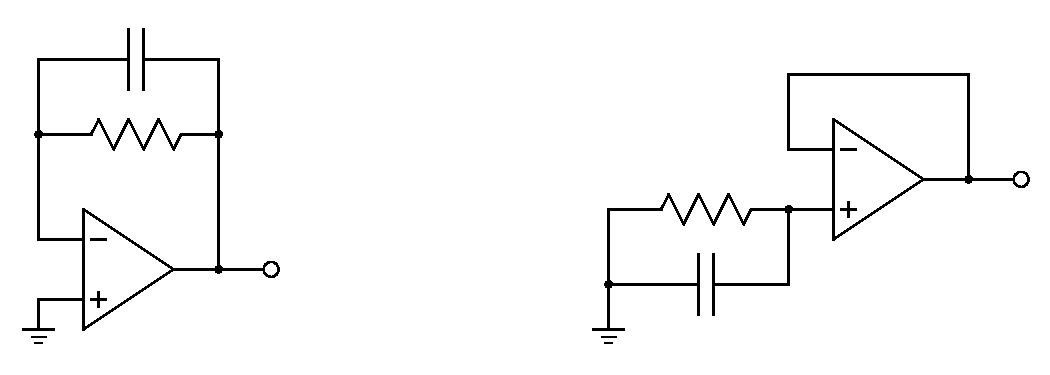
\includegraphics[scale=0.90]{opampInputBiasCurrentMeasurement}
\caption{حسابی ایمپلیفائر کے میلان برقی رو کا حصول}
\label{شکل__سوال_حسابی_میلان_برقی_رو}
\end{figure}
\begin{itemize}
\item
شکل-الف میں \عددی{V_o=\SI{-1.2}{\volt}} جبکہ شکل  الف     میں  \عددی{V_o=\SI{-1.21}{\volt}} پایا جاتا ہے۔مثبت داخلی سرے  کی میلان برقی رو \عددی{I_{B1}} اور منفی داخلی سرے  کی میلان برقی رو \عددی{I_{B2}}  اور ان کی سمتیں حاصل کریں۔
\item
\عددی{I_{B1}} اور \عددی{I_{B1}} سے \موٹا{انحرافی  برقی رو} حاصل کریں
\item
ایک حسابی ایمپلیفائر جس کی میلان برقی رو \عددی{\SI{100}{\nano \ampere}} کے لگ بھگ ہے کی مکمل درست میلان برقی رو حاصل کرنے کی خاطر شکل کو استعمال کیا جاتا ہے۔قابل ناپ خارجی اشارہ حاصل کرنے کی خاطر مزاحمت کی وہ قیمت تجویز کریں جس پر \عددی{v_o=\SI{1.5}{\volt}} کے لگ بھگ حاصل ہو۔
\end{itemize}
جوابات: \عددیء{\SI{200}{\nano \ampere}}،\عددی{\SI{201.66}{\nano \ampere}}، داخلی سروں سے باہر جانب، \عددی{\SI{15}{\mega \ohm}}
\انتہا{سوال}
%===============================
\ابتدا{سوال}
عفت بریخنہ نے انجنیئرنگ کے آخری سال میں آلاتی ایمپلیفائر کو استعمال کرتے ہوئے \موٹا{برقی قلب نگار}\حاشیہب{ecg} بنانے کا منصوبہ بنایا۔پہلے مرحلے میں انہوں نے شکل \حوالہ{شکل_آلاتی_ایمپلیفائر} میں \عددیء{R_1=\SI{250}{\ohm}}، \عددیء{R_2=\SI{2.5}{\kilo \ohm}} اور \عددی{R_3=R_4=\SI{39}{\kilo\ohm}} رکھ کر دائیں ہاتھ کی کلائی کو \عددی{v_1} جبکہ بائیں ہاتھ کی کلائی کو \عددی{v_2} کے ساتھ جوڑا۔ایسا کرنے کی خاطر \موٹا{ہم محوری تار}\فرہنگ{ہم محوری تار}\فرہنگ{تار!ہم محوری}\حاشیہب{co-axial cable} استعمال کئے گئے جن کی بیرونی تامبے کی چادر کو دور کے برقی زمین کے ساتھ جوڑا گیا تا کہ تار میں حساس اشارات پر بیرونی ناپسندیدہ برقی شور کے اثرات کم سے کم کئے جا سکیں۔دایاں ٹخنہ بھی برقی زمین کے ساتھ جوڑا گیا جس سے \عددی{\SI{50}{\hertz}} کا برقی شور نہایت کم ہو جاتا ہے۔حساس اشارات میں واپڈا کے \عددی{\SI{50}{\hertz}} کا شور عموماً پایا جاتا ہے جس سے نپٹنا ضروری ہوتا ہے۔

انہوں نے دیکھا کہ \عددی{v_o} پر دل کی دھڑکن کی چوٹی \عددی{\SI{0.6}{\volt}} تھی۔
\begin{itemize}
\item
اصل اشارہ \عددی{v_2 - v_1} کی قیمت دریافت کریں۔
\item
دل کا کون سا طرف دھڑکتے وقت مثبت برقی دباو پر تھا۔
\end{itemize}
\انتہا{سوال}
%=============

\ابتدا{سوال}
برقی قلب نگار میں برقی شور کے مسئلہ پر تحقیق کرنے کی خاطر عفت نے سائن نما داخلی اشارے کے حیطے کو سو گنا بڑھانے کی خاطر  شکل \حوالہ{شکل_منفی_ایمپلیفائر} میں دکھائے منفی حسابی ایمپلیفائر استعمال کیا جس میں  \عددی{R_1=\SI{1}{\kilo \ohm}} اور \عددی{R_2=\SI{100}{\kilo \ohm}} رکھے گئے۔بغیر زیادہ غور کئے \موٹا{لہر بین}\فرہنگ{لہر بین}\حاشیہب{oscilloscope} پر دیکھا گیا کہ \عددی{\SI{0.1}{\volt}} کا اشارہ بڑھاتے وقت دور نہایت عمدگی سے کام کرتے ہوئے \عددی{\SI{10}{\volt}} خارج کرتا ہے۔عفت نے امید رکھی کہ \عددی{\SI{10}{\milli \volt}} کے اشارے کو بھی دور خوش اسلوبی سے بڑھاتے ہوئے \عددی{\SI{1}{\volt}} خارج کرے گا۔\موٹا{لہر بین} میں غور سے دیکھتے ہوئے معلوم ہوا ہے کہ خارجی اشارے  کی مثبت چوٹی \عددی{\SI{1.2}{\volt}} جبکہ اس کی منفی چوٹی \عددی{\SI{-0.8}{\volt}} پر تھی۔

\begin{itemize}
\item
\عددی{v_s=\SI{0}{\volt}} کی صورت میں \عددی{v_o} کی کیا قیمت متوقع ہے۔
\item
اگر مسئلہ \موٹا{میلان برقی رو} کی وجہ سے پیدا ہوا ہو تب حسابی ایمپلیفائر کے مثبت داخلی سرے  پر  کتنی مزاحمت نسب کرنے سے مسئلہ حل ہو گا۔
\item
مثبت داخلی سرے  پر درکار مزاحمت نسب کرنے سے \عددی{v_s=\SI{0}{\volt}} کی صورت میں \عددی{v_o=\SI{0.19}{\volt}} حاصل ہوتا ہے۔یوں \موٹا{میلان برقی رو} کی وجہ سے خارجی اشارے میں \عددی{\SI{10}{\milli \volt}} کا فرق پیدا ہو رہا تھا۔\موٹا{میلان برقی رو} کی قیمت حاصل کریں۔
\item 
توقع کی جاتی ہے کہ بقایا \عددی{v_o=\SI{0.19}{\volt}} \موٹا{داخلی انحرافی برقی دباو} کی وجہ سے ہے۔استعمال کئے گئے حسابی ایمپلیفائر کی داخلی انحرافی برقی دباو \عددی{V_{OS}} حاصل کریں۔
\end{itemize}
جوابات: \عددیء{\SI{0.2}{\volt}}،  \عددیء{\SI{990}{\ohm}}، \عددیء{I_B=\SI{100}{\nano \ampere}} \عددی{\abs{V_{OS}}=\SI{1.88}{\milli \volt}}
\انتہا{سوال}
%==============================


%==============================
\ابتدا{سوال}
مال لادنے سے پہلے اور لادنے کے بعد ٹرک کا وزن   کرتے ہوئے لدے گئے مال کا وزن حاصل کیا جاتا ہے۔ٹرک کا وزن ناپنے کی خاطر \موٹا{لوڈ سیل}\فرہنگ{لوڈ سیل}\حاشیہب{load cell} استعمال کیا جاتا ہے جو در حقیقت \موٹا{ویٹ سٹون چکور}\فرہنگ{ویٹ سٹون چکور}\حاشیہب{Wheatstone bridge} پر مشتمل ہوتا ہے۔\موٹا{ویٹ سٹون چکور}\حاشیہد{ویٹ سٹون چکور کا نام چارلس ویٹ سٹون سے منسوخ ہے جنہوں نے اس کا استعمال عام بنایا} کو شکل \حوالہ{شکل__سوال_ویٹ_سٹون_چکور} میں دکھایا گیا ہے۔عام صورت میں اس کے چاروں مزاحمتوں کی قیمت برابر \عددی{R} ہوتی ہے۔وزن پڑنے پر ان میں سے ایک مزاحمت کی مزاحمت تبدیل ہو کر \عددی{R+\Delta R} ہو جاتی ہے۔ویٹ سٹون چکور سے اشارات \عددی{V_1} اور \عددی{V_2} حاصل کرتے ہوئے آلاتی ایمپلیفائر کو مہیا کئے جاتے ہیں جو ان میں نہایت باریک فرق \عددی{V_2-V_1} کو بڑھا کر خارج کرتا ہے۔ویٹ سٹون چکور کو آلاتی ایمپلیفائر کے ساتھ جوڑ کر خارجی اشارہ \عددی{v_o} کی مساوات حاصل کریں۔آلاتی ایمپلیفائر کو  صفحہ  \pageref{شکل_حسابی_آلاتی_ایمپلیفائر} پر شکل \حوالہ{شکل_حسابی_آلاتی_ایمپلیفائر} میں دکھایا گیا ہے۔

\begin{figure}
\centering
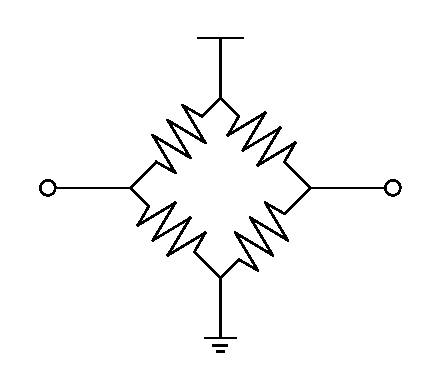
\includegraphics[scale=0.90]{wheatstoneBridge}
\caption{ویٹ سٹون چکور}
\label{شکل__سوال_ویٹ_سٹون_چکور}
\end{figure}
جواب:
ویٹ سٹون چکور کا
\begin{align*}
V_2-V_1=\frac{\Delta R}{4 \left(R+\frac{\Delta R}{2} \right)}  V_r
\end{align*}
کے برابر ہے۔اس کو آلاتی ایمپلیفائر کی افزائش سے ضرب دیتے ہوئے
%  
\begin{align*}
v_o=\frac{\Delta R}{4 \left(R+\frac{\Delta R}{2} \right)} \left(\frac{R_4}{R_3}\right) \left(1+\frac{2R_2}{R_1} \right) V_r
\end{align*}
حاصل ہوتا ہے۔

\انتہا{سوال}

%======================
\ابتدا{سوال}
مثبت حسابی ایمپلیفائر میں \عددی{R_1=\SI{1}{\kilo \ohm}} اور \عددی{R_2=\SI{14.7}{\kilo \ohm}} رکھے گئے۔\عددی{v_s=\SI{0.5}{\volt}} اشارے پر \عددی{v_o=\SI{7.85}{\volt}} متوقع ہے۔مزاحمتوں کے قیمتوں میں \عددی{\SI{\pm 5}{\percent}} غلطی  کے گنجائش کی صورت میں
\begin{itemize}
\item
\عددی{v_o}  کے ممکنہ حدود حاصل کریں۔
\item
کل غلطی اصل جواب کے کتنے فی صد ہے۔
\item
اگر کل غلطی کو \عددی{\SI{5}{\percent}} سے کم رکھا جائے تو مزاحمتوں کے قیمت میں زیادہ سے زیادہ کتنے فی صد غلطی قابل برداشت ہو گی۔
\end{itemize}

جوابات: خارجی اشارہ \عددی{\SI{7.15}{\volt}} تا \عددی{\SI{8.62368}{\volt}} ممکن ہے۔   زیادہ سے زیادہ \عددی{v_o} اس وقت حاصل ہو گا جب  \عددی{R_2} کی قیمت \عددی{\SI{5}{\percent}} زیادہ اور \عددی{R_1} کی قیمت  \عددی{\SI{5}{\percent}} کم ہو۔کل غلطی \عددی{\SI{18.77}{\percent}} ہے۔\عددی{\SI{\pm 1.33}{\percent}}

\انتہا{سوال}
%==============
\ابتدا{سوال}
غیر کامل حسابی ایمپلیفائر استعمال کرتے ہوئے  منفی حسابی ایمپلیفائر بنایا جاتا ہے جس میں \عددی{R_1=\SI{5}{\kilo \ohm}} اور \عددی{R_2=\SI{50}{\kilo \ohm}} رکھے جاتے ہیں۔غور کرنے پر معلوم ہوتا ہے کہ \عددی{\tfrac{v_o}{v_s}=\SI{-9.99}{\volt\per \volt}} حاصل ہوا ہے۔کامل حسابی ایمپلیفائر کا مساوی دور استعمال کرتے ہوئے  حسابی ایمپلیفائر کی \عددی{A_d} حاصل کریں۔

جوابات: \عددی{A_d=\SI{10989}{\volt\per \volt}}
\انتہا{سوال}
%====================
\ابتدا{سوال}
صفحہ \حوالہصفحہ{شکل_حسابی_مزاحمت_نما_ایمپلیفائر} پر مزاحمت نما ایمپلیفائر دکھایا گیا ہے۔\عددی{A_d \to \infty} کی صورت میں مزاحمت نما ایمپلیفائر کی
 \عددی{\tfrac{v_o}{i_s}=-R} کے برابر ہوتی ہے۔محدود \عددی{A_d} کی صورت میں  حسابی ایمپلیفائر کے کامل مساوی دور کے استعمال سے \عددی{\tfrac{v_o}{i_s}} اور داخلی مزاحمت حاصل کریں۔

جوابات: \عددی{\tfrac{v_o}{i_s}=-\tfrac{A_d R}{A_d+1}}، \عددی{R_{\textup{داخلی}}=\tfrac{R}{A_d+1}}
\انتہا{سوال}
%=====================================
\ابتدا{سوال}
ایک منفی حسابی ایمپلیفائر جس کی \عددی{A_d=\SI{60000}{\volt\per \volt}} ہو خطی خطے میں رہتے ہوئے \عددی{\SI{12}{\volt}} خارج کر رہا ہے۔کامل مساوی دور استعمال کرتے ہوئے منفی داخلی سرے  پر برقی دباو حاصل کریں۔اگر \عددی{A_d=\SI{1000}{\volt\per \volt}} ہوتا تب جواب کیا ہوتا۔
	
جوابات: \عددیء{\SI{-200}{\micro \volt}}،  \عددیء{\SI{-12}{\milli \volt}} 
\انتہا{سوال}
%===========================
\ابتدا{سوال}
لامحدود \عددی{A_d} کی صورت میں منفی حسابی ایمپلیفائر کی \عددی{A_v=-\tfrac{R_2}{R_1}} حاصل ہوتی ہے۔
\begin{itemize}
\item
محدود  \عددی{A_d} کی صورت میں صفحہ \حوالہصفحہ{شکل_حسابی_کامل_ماڈل} پر شکل \حوالہ{شکل_حسابی_کامل_ماڈل} میں دیے  کامل مساوی دور استعمال کرتے ہوئے \عددی{A_v} حاصل کریں۔ 
\item
لامحدود \عددی{A_d} کے جواب کی نسبت سے \عددی{A_v} میں غلطی کا فی صد حاصل کریں۔
\item
\عددی{A_d=\SI{10000}{\volt\per \volt}} کی صورت میں \عددی{\tfrac{R_2}{R_1}} کی وہ قیمت حاصل کریں جس پر \عددی{A_v} میں غلطی \عددی{\SI{0.1}{\percent}}ہو۔
\item
\عددی{A_d=\SI{10000}{\volt\per \volt}} کی صورت میں \عددی{R_2=\SI{9}{\kilo \ohm}} رکھتے ہوئے \عددی{R_1} کی وہ قیمت حاصل کریں جس پر \عددی{A_v} بالکل برابر \عددی{\SI{-50}{\volt\per \volt}} ہو۔اگر ایمپلیفائر میں \عددی{R_1=\SI{180}{\ohm}} پہلے سے نسب ہو تو \عددی{R_1} کے متوازی کتنی مزاحمت جوڑنے سے  بالکل صحیح درکار \عددی{R_1} حاصل ہوتی ہے۔

\end{itemize}

جوابات: \عددیء{A_v=\tfrac{-A_d R_2}{1+R_1 \left(A_d+1 \right)}}،  \عددیء{100 \left(\tfrac{R_1+R_2}{R_1 A_d +R_2} \right)}، \عددی{\tfrac{R_2}{R_1}=\tfrac{1}{0.111} \approx 9.009}۔آخری جواب سے ظاہر ہے کہ \عددی{A_v =\SI{-9}{\volt\per \volt}} سے زیادہ افزائش پر فرق \عددی{\SI{0.1}{\percent}} سے زیادہ ہو گا۔ \عددی{R_1=\SI{179.9819}{\ohm}}، \عددی{\SI{1.8}{\mega \ohm}}

\انتہا{سوال}
%==============
\ابتدا{سوال}
صفحہ \حوالہصفحہ{شکل_تکمل_کار} پر \موٹا{تکمل کار} دکھایا گیا ہے۔اس میں \عددی{R=\SI{14.7}{\kilo \ohm}} اور \عددی{C=\SI{0.01}{\micro \farad}} رکھیں۔حسابی ایمپلیفائر کی داخلی انحرافی برقی دباو \عددی{V_{OS}=\SI{2}{\milli \volt}} ہونے کی وجہ سے خارجی اشارہ صفر وولٹ سے کتنی دیر میں \عددی{V_{CC}=\SI{12}{\volt}} یا \عددی{V_{EE}=\SI{-12}{\volt}} تک پہنچ جائے گا۔اگر \عددی{C=\SI{0.1}{\micro \farad}}  کر دیا جائے تو جواب کیا ہو گا۔

جواب: \عددیء{\SI{0.882}{\second}}،  \عددیء{\SI{8.82}{\second}}۔ ان جوابات سے آپ دیکھ سکتے ہیں کہ داخلی اشارے کی عدم موجودگی یعنی \عددی{v_s=0}  کی صورت میں تکمل کار صفر وولٹ خارج نہیں کرتا بلکہ خارجی اشارہ مکمل مثبت یا مکمل منفی جانب پہنچنے کی کوشش کرتا ہے۔\عددی{RC} کی قیمت بڑھا کر  \عددی{v_o} کی رفتار آہستہ کرتے ہوئے اس عمل کو دیکھنے کی وضاحت دوسری جزو میں کی گئی۔

ایسا بدلتا داخلی اشارہ جس کے مثبت اور منفی حصے  برابر ہوں کے ایک چکر کا اوسط صفر ہوتا ہے۔تکمل کار ایسے اشارے کا تکمل لیتے ہوئے \عددی{V_{OS}} کا بھی تکمل لیتا ہے۔نتیجتاً تکمل کار کا خارجی اشارہ اوسطاً صفر وولٹ پر نہیں رہتا بلکہ اس کی مثبت چوٹی \عددی{V_{CC}} یا منفی چوٹی \عددی{V_{EE}} پر رہتے ہوئے یہ داخلی اشارے کا تکمل لیتا ہے۔

\انتہا{سوال}
%==================
\ابتدا{سوال}
صفحہ \حوالہصفحہ{حصہ_حسابی_عددی_سے_مماثل_کار} پر \موٹا{عددی سے مماثل کار} دکھایا گیا ہے۔\عددی{15_{10}} سروں  پر \عددی{\SI{-12}{\volt}} خارج کرنے کی خاطر \عددی{R'} کی قیمت حاصل کریں۔اس صورت \عددی{9_{10}}  پر کتنی مماثل برقی دباو خارج کیا جائے گا۔

جواب:\عددی{15_{10}} در حقیقت \عددی{1111_2} کو ظاہر کرتا ہے۔ \عددی{R'=1.28 R} درکار قیمت ہے۔\عددی{9_{10}} پر \عددی{v_o=\SI{-7.2}{\volt}} خارج کیا جائے گا۔

\انتہا{سوال}
%=======================
\ابتدا{سوال} \شناخت{سوال_حسابی_ٹریکٹر}
چالو ٹریکٹر پر بیٹھے ڈرائیور سے  ٹی وی پر نشریات کی خاطر سوال و جواب کیا جاتا ہے۔ٹریکٹر کی شور کو ختم کرنے کی خاطر دو مائک کا استعمال کیا جاتا ہے۔ایک مائک کو ڈرائیور کے منہ سے دو فٹ کے فاصلے پر جبکہ دوسرے کو منہ کے قریب رکھا جاتا ہے۔دور مائک صرف ٹریکٹر کا شور سنتے ہوئے \عددی{v_{s1}} اشارہ خارج کرتا ہے جبکہ قریب مائک ٹریکٹر کے شور کے ساتھ ساتھ ڈرائیور کی گفتگو بھی حاصل کرتے ہوئے اشارہ \عددی{v_{s2}} خارج کرتا ہے۔ٹریکٹر کے شور کو \عددی{V_t \cos \omega_t t} جبکہ ڈرائیور کے گفتگو کو \عددی{V_d \cos \omega_d t} لکھتے ہوئے
\begin{align*}
v_{s2}=V_t \cos \omega_t t +V_d \cos \omega_d t\\
v_{s1}=V_t \cos \omega_t t
\end{align*} 
اشارات حاصل ہوتے ہیں۔صفحہ \حوالہصفحہ{شکل_منفی_کار} پر دکھائے \موٹا{منفی کار} استعمال کرتے ہوئے شور سے پاک اشارہ حاصل کریں۔

جواب: تمام مزاحمت برابر قیمت کے رکھیں۔
\انتہا{سوال}
%==============
\ابتدا{سوال}
سوال \حوالہ{سوال_حسابی_ٹریکٹر} کے سوال و جواب لیتے وقت دیکھا گیا کہ دُور مائک میں نسبتاً زیادہ شور پایا جاتا ہے۔یوں
\begin{align*}
v_{s2}=V_t \cos \omega_t t +V_d \cos \omega_d t\\
v_{s1}=1.2 V_t \cos \omega_t t
\end{align*} 
اشارات حاصل ہوتے ہیں۔حل تجویز کریں۔

جواب: \عددی{\tfrac{R_4 \left(R_1+R_2 \right)}{R_1 \left(R_3+R_4 \right)}=1.2 \tfrac{R_2}{R_1}}
\انتہا{سوال}
%========================
\ابتدا{سوال}
لوہا پگھلانے والی بھٹی تخلیق دیتے وقت معلوم ہوا کہ \عددی{\SI{3}{\kilo \volt}} سے زیادہ برقی دباو پر مسائل پیدا ہوتے تھے۔برقی دباو  کو \عددی{\SI{3}{\kilo \volt}} سے کم رکھنے کی خاطر برقی دباو کا واپسی اشارہ درکار ہے۔واپسی اشارے کو شکل \حوالہ{شکل_سوال_بلند_برقی_دباو_اشارہ} کے منفی ایمپلیفائر میں \عددی{R_2 < R_1} رکھتے ہوئے حاصل کیا جاتا۔\عددی{\SI{3}{\kilo \volt}} پر \عددی{\SI{-6}{\volt}} کا اشارہ درکار ہے۔کسی بھی مزاحمت میں \عددی{\SI{30}{\milli \watt}} سے زیادہ برقی طاقت ضائع نہیں ہونا چاہئے۔ 
\begin{figure}
\centering
\includegraphics[scale=0.90]{potentialSensor}
\caption{بلند برقی دباو کے اشارے کا حصول}
\label{شکل_سوال_بلند_برقی_دباو_اشارہ}
\end{figure}
جوابات:\عددی{R_1=6R=500 R_2} اور \عددی{R=\SI{8.33}{\mega\ohm}}
\انتہا{سوال}
%=================
\ابتدا{سوال}
\عددیء{R_2=\SI{10}{\kilo\ohm}}، \عددیء{R_1=\SI{2}{\kilo\ohm}}، \عددی{V_{CC}=\SI{12}{\volt}} اور \عددی{V_{EE}=\SI{-12}{\volt}} رکھتے ہوئے منفی حسابی ایمپلیفائر کے داخلی سائن نما اشارے کی زیادہ سے زیادہ چوٹی کیا ہو گی جس پر ایمپلیفائر خطی خطے میں رہتا ہو۔مثبت ایمپلیفائر کے لئے بھی جواب حاصل کریں۔

جوابات: \عددی{\SI{2.4}{\volt}}  اور \عددی{\SI{2}{\volt}} 
\انتہا{سوال}
%================
\ابتدا{سوال}
\موٹا{مستطیلی پتلے اشارات}\فرہنگ{مستطیلی پتلا اشارہ}\حاشیہب{pulses} کے \موٹا{دورانیہ چڑائی}\فرہنگ{دورانیہ!چڑائی}\حاشیہب{rise time} سے مراد اشارے کا  \عددی{\SI{10}{\percent}} سے  \عددی{\SI{90}{\percent}} چوٹی تک پہنچنے کا دورانیہ ہے۔اسی طرح \موٹا{دورانیہ اترائی}\فرہنگ{دورانیہ!اترائی}\حاشیہب{fall time} سے مراد اشارے کا  چوٹی کے \عددی{\SI{90}{\percent}} سے \عددی{\SI{10}{\percent}} تک پہنچنے کا دورانیہ ہے۔

\عددی{\SI{5}{\volt}} چوٹی اور \عددی{\SI{1}{\micro \second}} \موٹا{دوری عرصے}\فرہنگ{دوری عرصہ}\حاشیہب{time period} والا \موٹا{چکور اشارہ}\حاشیہب{square wave} مستحکم کار کو فراہم کیا جاتا ہے۔دورانیہ چڑائی اور دارانیہ اترائی کا مجموعہ دوری عرصے کے \عددی{\SI{5}{\percent}} سے کم ہونا درکار ہے۔\موٹا{رفتار چال} حاصل کریں۔ 

جواب: \عددی{\SI{160}{\volt \per \micro \second}}
\انتہا{سوال}
%====================
\ابتدا{سوال}
صفحہ \حوالہصفحہ{شکل_جمع_و_منفی_کار} پر  \موٹا{جمع و منفی کار} دکھایا گیا ہے۔ \موٹا{جمع و منفی کار} کے مثبت داخلی سروں  سے جڑے \عددی{v_{j1}} تا \عددی{v_{js}} کو قصر دور کرتے ہوئے مزاحمت \عددی{R_{j1}} تا \عددی{R_{js}} کے داخلی سرے برقی زمین کے ساتھ جوڑتے ہوئے  دور کا خارجی اشارہ \عددی{v_{om}} حاصل کریں۔اسی طرح منفی داخلی سرے  قصر دور کرتے ہوئے خارجی اشارہ \عددی{v_{oj}} حاصل کریں۔تمام داخلی اشارات  کے موجودگی میں خارجی اشارہ \عددی{v_{oj}+v_{om}} کے برابر ہو گا۔اس طرح  مساوات  \حوالہ{مساوات_حسابی_جمع_و_منفی_کار} حاصل کریں۔
\انتہا{سوال}
%=====================
\ابتدا{سوال}
لامحدود \عددی{A_d} کی صورت میں \موٹا{مستحکم کار} کا خارجی اشارہ اس کے داخلی اشارے کے برابر ہوتا ہے۔\عددی{A_d=\SI{10000}{\volt \per \volt}} اور
\عددی{A_d=\SI{1000}{\volt \per \volt}} کی صورت میں خارجی اشارہ کتنے فی صد کم  یا زیادہ ہو گا۔

جوابات:خارجی اشارہ  \عددی{\SI{9.999e-3}{\percent}}، \عددی{\SI{0.0999}{\percent}} فی صد کم ہو گا۔
\انتہا{سوال}
%==============
\ابتدا{سوال}
\موٹا{منفی کار} اور \موٹا{جمع کار} میں تمام مزاحمت برابر ہونے کی صورت میں  \عددی{v_1} کو صفر وولٹ کرتے ہوئے \عددی{v_2} کو نظر آنے والا داخلی مزاحمت کیا ہو گا۔اسی طرح  \عددی{v_2} کو صفر وولٹ کرتے ہوئے \عددی{v_1} کو نظر آنے والا داخلی مزاحمت کیا ہو گا۔جواب بغیر حساب و کتاب کے بتلائیں۔

جوابات:\عددیء{2R}، \عددیء{R}، \عددیء{R}، اور \عددیء{R}
\انتہا{سوال}
%=================
\ابتدا{سوال}\شناخت{سوال_حسابی_مشترکہ_رد_کی_صلاحیت}
صفحہ \حوالہصفحہ{شکل_منفی_کار} پر \موٹا{منفی کار} دکھایا گیا ہے۔مساوات \حوالہ{مساوات_حسابی_منفی_کار} اس کی خارجی مساوات ہے۔داخلی اشارات
\begin{align*}
v_{s2}=v_m+\frac{v_f}{2}\\
v_{s2}=v_m-\frac{v_f}{2}
\end{align*}
کے داخلی اشارات منفی کار کو مہیا کئے جاتے ہیں جہاں \عددی{v_m} کو \موٹا{مشترکہ اشارہ}\فرہنگ{مشترکہ اشارہ}\حاشیہب{common mode signal} جبکہ \عددی{v_f} کو \موٹا{تفرق اشارہ}\فرہنگ{تفرق اشارہ}\حاشیہب{differential mode signal} کہتے ہیں۔خارجی مساوات کو
\begin{align}
v_o=A_{\textrm{مشترک}} v_m +A_{\textrm{تفرق}} v_f
\end{align}
صورت میں لکھیں۔مشترکہ افزائش تقسیمِ تفرق افزائش کو \موٹا{مشترکہ اشارہ رد کرنے کے صلاحیت}\فرہنگ{مشترکہ اشارہ رد کرنے کے صلاحیت}\حاشیہب{common mode rejection ratio CMRR} \تحریر{CMRR} کہتے ہیں۔ثابت کریں کہ
\begin{align*}
CMRR=\frac{A_{\textrm{تفرق}}}{A_{\textrm{مشترک}}}=\frac{1+\frac{1}{2}\left(\frac{R_1}{R_2}+\frac{R_3}{R_4} \right)}{\frac{R_1}{R_2}-\frac{R_3}{R_4}}
\end{align*}
کے برابر ہے۔

\انتہا{سوال}
%===================
\ابتدا{سوال}
منفی کار بناتے وقت \عددی{\tfrac{R_2}{R_1}=\tfrac{R_3}{R_4}} رکھا جاتا ہے جس سے  اس کی \موٹا{مشترکہ اشارہ رد کرنے کے صلاحیت} کی قیمت لامحدود حاصل ہوتی ہے۔حقیقی مزاحمتوں کی قیمت ان کے پکارے گئے قیمتوں سے اوپر نیچے ہوتیں ہیں۔سوال \حوالہ{سوال_حسابی_مشترکہ_رد_کی_صلاحیت} میں حاصل جواب کو استعمال کرتے ہوئے ثابت کریں کہ ایسی صورت میں  کم سے کم  \موٹا{مشترکہ اشارہ رد کرنے کے صلاحیت} کی قیمت \عددی{\tfrac{A+1+\epsilon^2}{4 \epsilon}} کے برابر ہو گی جہاں \عددی{A=\tfrac{R_2}{R_1}=\tfrac{R_4}{R_3}} کے برابر ہے اور مزاحمت کے قیمتوں میں \عددی{\SI{5}{\percent}} غلطی کے لئے \عددی{\epsilon = 0.05} ہو گا۔

\عددی{R_1=R_3=\SI{1}{\kilo \ohm}} اور \عددی{R_2=R_4=\SI{21}{\kilo \ohm}} کی صورت میں اگر مزاحمتوں کے قیمتوں میں \عددی{\SI{\mp 5}{\percent}}  غلطی کی گنجائش ہو تب  \موٹا{مشترکہ اشارہ رد کرنے کے صلاحیت} کی قیمت کیا حاصل ہو گی۔\عددی{\SI{\mp 0.1}{\percent}} کی صورت میں جواب کیا ہو گا۔ 

جوابات: 110،  5500
\انتہا{سوال}
%==================

\ابتدا{سوال}
\عددی{\SI{\mp 12}{\volt}} پر چلنے والے ایک حسابی ایمپلیفائر کا خارجی اشارہ \عددی{\SI{-10.5}{\volt}} تا  \عددی{\SI{+10.5}{\volt}} بغیر بگڑے تبدیل ہو سکتا ہے۔اسے استعمال کرتے ہوئے \عددی{A_v=\SI{-40}{\volt \per \volt}} کا منفی حسابی ایمپلیفائر بنایا جاتا ہے۔داخلی اشارے کی وہ چوٹی \عددی{V_p} حاصل کریں جس پر خارجی اشارہ بگڑ جائے گا۔

جواب: \عددی{\abs{V_p} > \SI{0.2625}{\volt}}
\انتہا{سوال}
%========================

